\documentclass[12pt,openany]{book}


% Load packages
\usepackage[utf8]{inputenc} % for unicode input
 \usepackage{microtype}
\usepackage{geometry} % for page layout
\usepackage{hyperref} % for hyperlinks
\usepackage{tocbibind} % includes the bibliography in the table of contents
\usepackage{amsmath} % for advanced math formatting
\usepackage{amsfonts} % for mathematical fonts
\usepackage{amssymb} % for mathematical symbols
\usepackage{lipsum} % generates filler text
\usepackage{fancyhdr}
\usepackage{amsthm} % for theorem environments
\usepackage{amsmath}
\usepackage[table]{xcolor} % for cell coloring
\usepackage{colortbl} % for cell coloring
\usepackage{graphicx} % for scaling the table
\usepackage{booktabs} % For professional looking tables
\usepackage[table]{xcolor} % For cell coloring
\usepackage[normalem]{ulem} % For underlining
\usepackage[document]{ragged2e}
\usepackage{tikz}
\usepackage{algorithm}
\usepackage{algpseudocode}
\usepackage{wrapfig}
\usepackage{circuitikz}
\usepackage{tikz}
\usepackage{caption}
\usepackage{venndiagram}
\usepackage{multicol} % Import multicol package
\usepackage{amsmath}
\usepackage{colortbl}
\usepackage{hhline}

\usepackage{listings}
\usepackage{adjustbox}


\usepackage{hyperref}



%%%%%%%%%%%%%%%%%%%%%%%%%%%%%


\usetikzlibrary{circuits.logic.US}
\usetikzlibrary{arrows.meta, positioning, calc}
\usetikzlibrary{fit} % Add the missing TikZ library

\usetikzlibrary{arrows.meta,calc,decorations.markings,math,arrows.meta}

% Document geometry (page size, margins)
\geometry{a4paper, left=25mm, right=25mm, top=30mm, bottom=30mm}
% Custom page style for centered page numbers
\pagestyle{fancy}
\fancyhf{} % Clear all header and footer fields
\fancyhead[RE]{\leftmark} % 'LE' for Left Even pages - Chapter number and name
\fancyhead[RO]{Notes by Ali EL AZDI} % 'LO' for Left Odd pages - Custom message
\fancyfoot[CE,CO]{\thepage} % Centered page number in the footer for both even and odd pages

\renewcommand{\headrulewidth}{0pt}
\renewcommand{\footrulewidth}{0pt}
\newcommand*\xor{\oplus}
\newcommand{\minidash}{\text{-}}

\makeatletter
\newcommand{\vspacer}[1]{%
  % Check if we are in vertical mode
  \ifvmode
    % Insert the requested vertical space
    \vskip#1\relax
  \else
    % We are in horizontal mode (within a paragraph)
    \@bsphack
    \vadjust{%
      \vskip#1\relax
    }%
    \@esphack
  \fi
}
\makeatother

%%%%%%%%%%%%%%%%%%% VHDL CODE STYLING %%%%%%%%%%%%%%%%%%%%%%%%%%%%%
\usepackage{listings}
\usepackage{xcolor}
\usepackage{courier}

% Define your colors here
\definecolor{keywordcolor}{rgb}{0.5,0.0,0.33}
\definecolor{backgroundcolor}{rgb}{0.95,0.95,1.0}
\definecolor{commentcolor}{rgb}{0.129,0.384,0.529}
\definecolor{stringcolor}{rgb}{0.16,0.00,1.00}
\definecolor{rulecolor}{rgb}{0.46,0.43,0.5}
\definecolor{codegray}{rgb}{0.5,0.5,0.5} % Add this line

\lstdefinestyle{vhdlstyle}{
  language=VHDL,
  basicstyle=\ttfamily\footnotesize,
  backgroundcolor=\color{backgroundcolor},
  commentstyle=\color{commentcolor}\ttfamily, % Add \ttfamily to ensure comments are in typewriter font
  morecomment=[l][\color{commentcolor}\ttfamily]{//}, % Line comment in VHDL
  morekeywords={module,input,output,wire,endmodule,endcase,default,tri,assign,always},
  keywordstyle=\color{keywordcolor},
stringstyle=\color{stringcolor},
  showstringspaces=false,
  frame=single,
  rulecolor=\color{rulecolor}, % Frame color
  breaklines=true,
  numbers=left,
  numberstyle=\tiny\color{codegray},
  tabsize=2
}

% Define your custom environment
\lstnewenvironment{vhdl}
  {\lstset{style=vhdlstyle}}
  {}





%%%%%%%%%%%%%%%%%%%%%%%%%%%%%%%%%%%%%%%%%%%%%%%%%%%%%%%%
% Document begins
\begin{document}


% Title Page
\begin{titlepage}
	\centering
	\vspace*{1cm}
	    
	    
	\vspace{0.5cm}
	\Huge
	Fundamentals of digital systems
	\vspace{10px}
	\newline
	\text{ \large Ali EL AZDI}
	
	
	\text{ \Large IC BA2 - Mirjana Stojilović}
	    
	\vfill
	\large
	February 19, 2024
	
	    
\end{titlepage}
\begin{center}
	\vspace*{1cm}
	\textbf{Introduction}
	\newline
	\paragraph[short]{}{This document is designed to offer a LaTeX-styled overview of the Fundamentals of Digital Systems course, emphasizing brevity and clarity. Should there be any inaccuracies or areas for improvement, please do not hesitate to reach out to me at ali.elazdi@epfl.ch for corrections. Hoping to provide an experience similar to the one provided by past generations of students in other subjects. Also, for the latest version of this pdf file, as the update on drive may take some time, you can find it on my github repository at the following link: \url{https://github.com/elazdi-al/FDS/blob/main/FDS.pdf}}
\end{center}


% Table of Contents
\tableofcontents

% List of Figures (Uncomment if needed)
% \listoffigures

% List of Tables (Uncomment if needed)
% \listoftables

\mainmatter% Chapter 1
\chapter{Number Systems}


% Section 1.1
\section{Digital Representations}
\begin{itemize}
	\item[] In a digital representation, a number is represented by an ordered n-tuple:
	      \begin{itemize}
	      	\item[] The n-tuple is called a \textbf{digit vector}, each element is a \textbf{digit}
	      	\item[] The number of digits $n$ is called the precision of the representation. (careful! leftward indexing)
	      	              
	      	          
	      \end{itemize}
\end{itemize}
\[ X  = (X _{n-1}, X _{n-1}, \ldots, X _{0}) \]
\begin{itemize}
	\item[] Each digit is given \textbf{a set of values} $D_{i}$ 
	      (eg. For base 10 representation of numbers, $D_i = \{0,1,2, \dots, 9\}$)
	\item[] The \textbf{set size}, the maximum number of representable digit vectors is: $K = \prod_{i=0}^{n-1} |D_{i}|$
\end{itemize}



  
  




\subsection{(Non)Redundant Number Systems}
A number system is nonredundant if each digit-vector represents a different integer

\subsection{Weighted Number Systems}
The rule of representation if a Weighted (Positional) Number Systems is as follows :
$$\;\displaystyle\sum_{i=0}^{n-1} X_{i}W_{i}$$ where $$W = (W_{n-1}, W_{n-2}, \dots, W_{0})$$

\subsection{Radix Systems}
When weights are in this format : 
\[
	\begin{cases}
		$$W_{0} = 1                                                \\
		W_{i+1} = W_{i}R_{i} \;\; \text{with } 1 \leq i \leq n-1$$ 
	\end{cases} \]
	
	
	
	
	
	Also written :
	$W_{0} = 1, \; \prod_{j=0}^{i-1} R_{j}$
	
	\subsection{Fixed and Mixed-Radix Number Systems}
	\begin{itemize}
		\item[] In a \textbf{fixed-radix system}, all elements of the radix-vector have the same value \( r \) (\textit{the radix})
		\item[] The weight vector in a fixed-radix system is given by:
		      \begin{equation*}
		      	W = \left( r^{n-1}, r^{n-2}, \ldots, r^2, r, 1 \right)
		      \end{equation*}
		      and the integer \( x \) becomes:
		      \begin{equation*}
		      	x = \sum_{i=0}^{n-1} X_i \times r^i
		      \end{equation*}
		\item[] In a \textbf{mixed-radix system}, the elements of the radix-vector differ
	\end{itemize}
	\subsection*{Example: Decimal Number System}
	The decimal number system has the following characteristics:
	\begin{itemize}
		\item[-] Radix \(r = 10\), it's a fixed-radix system.
	\end{itemize}
	The weight vector \(W\) is defined as:
	\begin{equation*}
		W = \left(10^{n-1}, 10^{n-2}, \ldots, 10^2, 10, 1\right)
	\end{equation*}
	An integer \(x\) in this system is represented by:
	\begin{equation*}
		x = \sum_{i=0}^{n-1} X_i \times 10^i
	\end{equation*}
	For example:
	\begin{equation*}
		854703 = 8 \times 10^5 + 5 \times 10^4 + 4 \times 10^3 + 7 \times 10^2 + 0 \times 10^1 + 3 \times 10^0
	\end{equation*}
	
	\subsubsection{Examples of Fixed and Mixed radix systems}
	\begin{description}
		\item[Fixed:] The base of number systems.
		\begin{itemize}
			\item Decimal – radix 10
			\item Binary – radix 2
			\item Octal – radix 8
			\item Hexadecimal – radix 16
		\end{itemize}
		\item[Mixed:] An example of a mixed radix representation, such as time:
		\begin{itemize}
			\item Radix-vector \(R = (24, 60, 60)\)
			\item Weight-vector \(W = (3600, 60, 1)\)
		\end{itemize}
	\end{description}
	
	\subsection{Canonical Number Systems}
	
	\begin{itemize}
		\item[] In a \textbf{canonical number system}, the set of values for a digit \( D_i \) is with \( |D_i| = R_i \), the corresponding element of the radix vector
		      \begin{equation*}
		      	D_i = \{0, 1, \ldots, R_i - 1\}
		      \end{equation*}
		\item[] Canonical digit sets with fixed radix:
		      \begin{itemize}
		      	\item Decimal: \{0, 1, \ldots, 9\}
		      	\item Binary: \{0, 1\}
		      	\item Hexadecimal: \{0, 1, 2, \ldots, 15\}
		      \end{itemize}
		\item[] Range of values of \( x \) represented with \( n \) fixed-radix-\( r \) digits:
		      \begin{equation*}
		      	0 \leq x \leq r^n - 1
		      \end{equation*}
		      A system with fixed positive radix r and a canonical set of digit values is called a radix-r conventional number system.
	\end{itemize}
	\newpage
	\section{Binary/Octal/Hexadecimal to/from Decimal}
	\section*{Conversion Table}
	\begin{itemize}
		\item[] The hexadecimal system supplements 0-9 digits with the letters A-F.
		      \vspace{-5px}
		\item[] \textit{Remark.} Programming languages often use the prefix 0x to denote a hexadecimal number.
	\end{itemize}
	
	% Define the color for the table cells
	\definecolor{cellblue}{rgb}{0.88, 0.94, 0.97}
	\definecolor{cellpink}{rgb}{0.96, 0.88, 0.89}
	\definecolor{cellgreen}{rgb}{0.906, 1, 0.831}
	\vspace{-20px}
	
	\begin{table}[ht]
		\centering
		\caption*{Conversion table up to 15.}
		\vspace{10px}
		\label{my-label}
		\begin{tabular}{@{}cccc@{}}
			\toprule
			\textbf{Decimal} & \textbf{Binary}           & \textbf{Octal}         & \textbf{Hexadecimal}  \\ \midrule
			0                & \cellcolor{cellgreen}0000 & \cellcolor{cellblue}00 & \cellcolor{cellpink}0 \\
			1                & \cellcolor{cellgreen}0001 & \cellcolor{cellblue}01 & \cellcolor{cellpink}1 \\
			2                & \cellcolor{cellgreen}0010 & \cellcolor{cellblue}02 & \cellcolor{cellpink}2 \\
			3                & \cellcolor{cellgreen}0011 & \cellcolor{cellblue}03 & \cellcolor{cellpink}3 \\
			4                & \cellcolor{cellgreen}0100 & \cellcolor{cellblue}04 & \cellcolor{cellpink}4 \\
			5                & \cellcolor{cellgreen}0101 & \cellcolor{cellblue}05 & \cellcolor{cellpink}5 \\
			6                & \cellcolor{cellgreen}0110 & \cellcolor{cellblue}06 & \cellcolor{cellpink}6 \\
			7                & \cellcolor{cellgreen}0111 & \cellcolor{cellblue}07 & \cellcolor{cellpink}7 \\
			8                & \cellcolor{cellgreen}1000 & \cellcolor{cellblue}10 & \cellcolor{cellpink}8 \\
			9                & \cellcolor{cellgreen}1001 & \cellcolor{cellblue}11 & \cellcolor{cellpink}9 \\
			10               & \cellcolor{cellgreen}1010 & \cellcolor{cellblue}12 & \cellcolor{cellpink}A \\
			11               & \cellcolor{cellgreen}1011 & \cellcolor{cellblue}13 & \cellcolor{cellpink}B \\
			12               & \cellcolor{cellgreen}1100 & \cellcolor{cellblue}14 & \cellcolor{cellpink}C \\
			13               & \cellcolor{cellgreen}1101 & \cellcolor{cellblue}15 & \cellcolor{cellpink}D \\
			14               & \cellcolor{cellgreen}1110 & \cellcolor{cellblue}16 & \cellcolor{cellpink}E \\
			15               & \cellcolor{cellgreen}1111 & \cellcolor{cellblue}17 & \cellcolor{cellpink}F \\\bottomrule
		\end{tabular}
	\end{table}
	    
	
	\subsection{Convertion examples}    
	\subsubsection*{Binary to Decimal:}
	
	    
	To convert a binary number to decimal, multiply each bit by two raised to the power of its position number, starting from zero on the right.
	
	
	
	\begin{flalign*}
		& \text{Binary:}       & \underline{1} \underline{0} \underline{1} \underline{1} & \\
		& \text{Decimal:}      & 1 \times 2^3 + 0 \times 2^2 + 1 \times 2^1 + 1 \times 2^0 = 8 + 0 + 2 + 1 = 11 &
	\end{flalign*}
	    
	\newpage
	
	\subsubsection*{Decimal to Binary:}
	
	Let's convert the decimal number \( 25_{10} \) to binary.
	
	\begin{tabular}{rclr}
		$25 \div 2$ & = & 12 & remainder 1 (LSB) \\
		$12 \div 2$ & = & 6  & remainder 0       \\
		$6 \div 2$  & = & 3  & remainder 0       \\
		$3 \div 2$  & = & 1  & remainder 1       \\
		$1 \div 2$  & = & 0  & remainder 1 (MSB) \\
	\end{tabular}
	
	\vspace*{10px}
	Thus, the binary representation of \( 25_{10} \) is \( 11001_2 \) (reading the remainders in reverse).
	   
	
	\vspace*{10px}
	\textit{Personal Remark} The trick is always to try to answer the question, what's the biggest power of 2 I need to form the number?. For 157, the biggest power would be $2^{7} = 128$, then $128+64$ is greater than 157, $128 + 32$ is still greater than 157, $128 + 16 = 144$, and so on to obtain : $128+16+8+4+1=157$ which can be written as $2^7 + 2^4 + 2^3 + 2^2 + 2^0 = 157$. Written in binary as $ 10011101_{2} $
	
	\subsubsection*{Octal to Decimal:}
	    
	Each octal digit is converted to decimal by multiplying it by eight raised to the power of its position number, starting from zero on the right.
	    
	\begin{flalign*}
		& \text{Octal:}        & \underline{2} \underline{5} \underline{7} & \\
		& \text{Decimal:}      & 2 \times 8^2 + 5 \times 8^1 + 7 \times 8^0 = 128 + 40 + 7 = 175 &
	\end{flalign*}
	\subsubsection*{Decimal to Octal:}
	To convert the decimal number \(93_{10}\) to octal.
	    
	\begin{tabular}{rclr}
		$93 \div 8$ & = & 11 & remainder 5 \\
		$11 \div 8$ & = & 1  & remainder 3 \\
		$1 \div 8$  & = & 0  & remainder 1 \\
	\end{tabular}
	    
	\vspace*{10px}
	Thus, the octal representation of \(93_{10}\) is \(135_8\) (reading the remainders in reverse).
	    
	\subsubsection*{Hexadecimal to Decimal:}
	
	To convert the hexadecimal number \( \text{1A3}_{16} \) to decimal.
	
	\begin{flalign*}
		& \text{Hexadecimal:}       & \underline{1} \underline{A} \underline{3} & \\
		& \text{Decimal:}           & 1 \times 16^2 + A \times 16^1 + 3 \times 16^0 & \\
		&                           & 1 \times 256 + 10 \times 16 + 3 \times 1 & \\
		&                           & 256 + 160 + 3 & \\
		&                           & 419 &
	\end{flalign*}
	
	Here, \( \text{A} \) in hexadecimal corresponds to \( 10 \) in decimal.
	
	
	
	    
	
	
	    
	\subsubsection*{Decimal to Hexadecimal:}
	  
	To convert the decimal number \(291_{10}\) to hexadecimal.
	    
	\begin{tabular}{rclr}
		$291 \div 16$ & = & 18 & remainder 3 \\
		$18 \div 16$  & = & 1  & remainder 2 \\
		$1 \div 16$   & = & 0  & remainder 1 \\
	\end{tabular}
	    
	\vspace*{10px}
	Thus, the hexadecimal representation of \(291_{10}\) is \(123_{16}\) (reading the remainders in reverse).
	    
	
	
	\section{Octal/Hexadecimal to/from Binary}
	\section*{Bit-Vector Representation Summary}
	
	\begin{itemize}
		\item Digit-vectors for binary, octal, and hexadecimal systems are represented using bit-vectors. In binary, 0 and 1 are directly represented as 0 and 1.
		\item In systems like octal or hexadecimal, a digit is a bit-vector of length \( k \), where \( k \) is the number of bits needed to represent the base.$$k=\log_{2}(r)$$
		      with r the radix of the system (eg. 8 for octal convertion).
		\item For example, the hexadecimal digit \( B \) is represented as the bit-vector 1101 in binary. \textit{We obtain a length 4 bit-vector because the base is 16 and \( \log_{2}(16) = 4 \)}
	\end{itemize}
	
	\subsubsection*{Binary to Octal:}
	
	To convert a binary number to octal, group every three binary digits into a single octal digit, because \( k = \log_2 8 = 3 \).
	    
	\begin{flalign*}
		& \text{Binary:}       & \underline{010}\,\underline{000}\,\underline{100}\,\underline{110} & \\
		& \text{Octal:}        & 2_8\,0_8\,4_8\,6_8 &
	\end{flalign*}
	    
	\subsubsection*{Binary to Hexadecimal:}
	    
	To convert a binary number to hexadecimal, group every four binary digits into a single hexadecimal digit, because \( k = \log_2 16 = 4 \).
	    
	\begin{flalign*}
		& \text{Binary:}       & \underline{1011}\,\underline{1110}\,\underline{1010}\,\underline{1101} & \\
		& \text{Hexadecimal:}  & B_{16}\,E_{16}\,A_{16}\,D_{16} &
	\end{flalign*}
	    
	
	
	\subsubsection*{Octal to Hexadecimal:}
	Convert the octal number to binary, then group the binary digits in sets of four and convert each group to its hexadecimal equivalent.
	    
	\begin{flalign*}
		& \text{Octal:}        & \underline{2} \underline{5} \underline{7} & \\
		& \text{Binary:}       & 010 \, 101 \, 111 & \text{ (Octal to binary)} \\
		& \text{Binary grouped:} & \underline{0101} \, \underline{0111} & \\
		& \text{Hexadecimal:}  & 5 \, 7 & \text{ (Binary to hexadecimal)}
	\end{flalign*}    
	
	\section{Representation of
	Signed Integers}
	\subsection{Sign-Magnitude Representation (SM)}
	
	A signed integer \( x \) is represented by a pair \( (x_s, x_m) \), where \( x_s \) is the \textit{sign} and \( x_m \) is the \textit{magnitude} (positive integer).
	
	\begin{itemize}
		\item[] The sign (positive, negative) is represented by a the most significant bit (MSB) of the digit vector:
		      \begin{itemize}
		      	\item[] \( 0 \rightarrow \) positive
		      	\item[] \( 1 \rightarrow \) negative
		      \end{itemize}
		\item[] The magnitude can be represented as any positive integer. In a conventional radix-\( r \) system, the range of \( n \)-digit magnitude is:
		      \[ 0 \leq x_m \leq r^n - 1 \]
	\end{itemize}
	
	\begin{itemize}
		\item[-] Examples:
		      \begin{align*}
		      	01010101_2 & = +85_{10}  \\
		      	01111111_2 & = +127_{10} \\
		      	00000000_2 & = +0_{10}   \\
		      	11010101_2 & = -85_{10}  \\
		      	11111111_2 & = -127_{10} \\
		      	10000000_2 & = -0_{10}   \\
		      \end{align*}
	\end{itemize}
	\newpage
	Note: The Sign-and-Magnitude representation is considered a redundant system because both \( 00000000_2 \) and \( 10000000_2 \) represent zero.
	
	\begin{itemize}
		\item[] \textit{SM} consists of an equal number of positive and negative integers.
		\item[] An \( n \)-bit integer in sign-and-magnitude lies within the range \textit{(because of 0's double representation and that MSB is used for the sign)}: 
		      $$ [-\left(2^{n-1} - 1\right), +\left(2^{n-1} - 1\right)] $$ 
		\item[] Main disadvantage of SM: complex digital circuits for arithmetic operations (addition, subtraction, etc.).
	\end{itemize}
	
	\section{True-and-Complement (TC)}
	
	\subsection{Mapping}
	\begin{itemize}
		\item[] A signed integer \( x \) is represented by a positive integer \( x_R \), \( C \) is a positive integer called the \textit{complementation constant}.
		      \[ x_R \equiv x \mod C \]
		          
		\item[] For \( |x| < C \), by the definition of the modulo function, we have:
		      \[
		      	x_R = 
		      	\begin{cases} 
		      		x               & \text{if } x \geq 0 \quad \text{(True form)}    \\
		      		C - |x| = C + x & \text{if } x < 0 \quad \text{(Complement form)} 
		      	\end{cases}
		      \]
	\end{itemize}
	
	\subsection{Unambiguous Representation}
	To have an unambiguous representation, the two regions should not overlap, translating to the condition:
		$\forall x, \max |x| < \frac{C}{2} $

	
	
	\subsection{Converse Mapping}
	\begin{itemize}
		\item[] Converse mapping:
		      \[
		      	x = 
		      	\begin{cases} 
		      		x_R     & \text{if } x_R < \frac{C}{2} \quad \text{(Positive values)} \\
		      		x_R - C & \text{if } x_R > \frac{C}{2} \quad \text{(Negative values)} 
		      	\end{cases}
		      \]
		\item[] When \( x_R = \frac{C}{2} \), it is usually assigned to \( x = -\frac{C}{2} \).
		\item[] Asymmetrical representation simplifies sign detection.
		      
	\end{itemize}
	
	\section{Two's Complement System}
	This is the True-and-Compelement system with \( C = 2^n \), where \( n \) is the number of bits used to represent the integer.
	\begin{itemize}
		\item[] Range is asymmetrical:
		      \[ -2^{n-1} \leq x \leq 2^{n-1} - 1\]
		\item[] The representation of zero is unique.
	\end{itemize}
	
	
	\subsection{Sign Detection in Two's Complement System}
	
	\begin{itemize}
		\item[] Since $|x| < C/2$ and assuming the sign is 0 for positive and 1 for negative numbers:
	\end{itemize}
	
	\[
		\text{sign}(x) = 
		\begin{cases} 
			0 & \text{if } x_R < C/2    \\
			1 & \text{if } x_R \geq C/2 
		\end{cases}
	\]
	
	\begin{itemize}
		\item[] Therefore, the sign is determined from the most-significant bit:
	\end{itemize}
	
	\[
		\text{sign}(x) = 
		\begin{cases} 
			0 & \text{if } x_{n-1} = 0 \\
			1 & \text{if } x_{n-1} = 1 
		\end{cases}
		\quad \text{equivalent to} \quad \text{sign}(x) = x_{n-1}
	\]
	\subsection{Mapping from Bit-Vectors to Values}
	The value of an integer represented by a bit-vector $b_{n-1}b_{n-2}\ldots b_1b_0$ can be universally expressed as:
	\[
		\text{Value} = (-2^{n-1} \cdot b_{n-1}) + \sum_{i=0}^{n-2} b_i \cdot 2^i
	\]
	where $b_{n-1}$ is the MSB (sign bit) and is $0$ for non-negative numbers and $1$ for negative numbers.
	
	\subsubsection{Examples}
	\begin{itemize}
		\item[] $X = 011011_2 = 0 \cdot 2^5 + 1 \cdot 2^4 + 1 \cdot 2^3 + 0 \cdot 2^2 + 1 \cdot 2^1 + 1 \cdot 2^0 = 16 + 8 + 2 + 1 = 27_{10}$
		\item[] $X = 11011_2 = -1 \cdot 2^4 + 1 \cdot 2^3 + 0 \cdot 2^2 + 1 \cdot 2^1 + 1 \cdot 2^0 = -16 + 8 + 2 + 1 = -5_{10}$
		\item[] $X = 10000000_2 = -1 \cdot 2^7 = -128_{10}$
		\item[] $X = 10000011_2 = -1 \cdot 2^7 + 1 \cdot 2^1 + 1 \cdot 2^0 = -128 + 2 + 1 = -125_{10}$
	\end{itemize}
	  
	\subsection{Change of Sign in Two's Complement System}
	
	
	The two's complement system represents negative numbers by inverting the bits of their positive counterparts and adding one. This process is equivalent to subtracting the number from $2^n$.
	  
	For an $n$-bit number $x$:
	\[
		z = -x = (\sim x) + 1 = C - x_R
	\]
	where $(\sim x)$ is the bitwise NOT of $x$ and $x_R$ is the decimal representation of $x$.
	  
	
	  
	
	
	\subsection*{Examples}
	Converting $+17$ to $-17$:
	\[
		\begin{aligned}
			+17_{10} & = 00010001_2                             \\
			-17_{10} & = \overline{00010001_2} + 1 = 11101111_2 \\
			2^8 - 17 & = 256 - 17 = 239 = 11101111_2            
		\end{aligned}
	\]
	  
	Converting $-99$ to $+99$:
	\[
		\begin{aligned}
			-99_{10} &= 10011101_2 \\
			+99_{10} & = \overline{10011101_2} + 1 = 01100011_2 &   & (TC) \\
			2^8 - 99 &= 256 - 99 = 157 = 01100011_2 \; (Substracting \; 99 \; from \; 256)
		\end{aligned}
	\]
	
	\section{Range Extension and Arithmetic Shifts}
	\subsection{Range Extension}
	
	\begin{itemize}
		\item[] Performed when a value \( x \) represented by a digit-vector of \( n \) bits needs to be represented by a digit-vector of \( m \) bits, where \( m > n \).
		\item[] \( x \) is represented as:
			  \begin{align*}
				  X & = (X_{n-1}, X_{n-2}, \ldots, X_1, X_0) \\
				  Z & = (Z_{m-1}, Z_{m-2}, \ldots, Z_1, Z_0) 
			  \end{align*}
	\end{itemize}
	
	\small \section{Range Extension Algorithm in Sign-and-Magnitude}
	\begin{itemize}
		\item[] In sign-and-magnitude system, the range-extension algorithm is defined as:
			  \begin{align*}
				  z_s & = x_s \text{ (sign bit)}                          \\
				  Z_i & = 0 \quad \text{for } i = m - 1, m - 2, \ldots, n \\
				  Z_i & = X_i \quad \text{for } i = n - 1, \ldots, 0      
			  \end{align*}
		\item[] Example: Consider \( X = 11010101_2 = -85_{10} \).
		\item[] The algorithm extends the range of \( X \) by adding zeros to the left of the most significant bit, preserving the sign bit.
	\end{itemize}
	
	
	\subsection{Arithmetic Shifts}
	
	\begin{itemize}
		\item[] Two elementary transformations often used in arithmetic operations are scaling (multiplying and dividing) by the radix.
		\item[] In the conventional radix-2 number system for integers:
			  \begin{itemize}
				  \item[] Left arithmetic shift: multiplication by 2, expressed as \( z = 2x \).
				  \item[] Right arithmetic shift: division by 2, expressed as \( z = x/2 \), with rounding towards zero when \( x \) is negative.
			  \end{itemize}
	\end{itemize}
	
	\subsection{Left Arithmetic Shift in Sign-and-Magnitude System}
	
	\begin{itemize}
		\item[] Algorithm (assuming the overflow does not occur):
			  \begin{align*}
				  z_s     & = x_s \text{ (sign bit retained)}                      \\
				  Z_{i+1} & = X_i, \quad \text{for } i = 0, \ldots, n-2            \\
				  Z_0     & = 0 \text{ (insert zero at the least significant bit)} 
			  \end{align*}
			  \subsubsection*{Example:}
			  \begin{itemize}
				  \item[] Given \( X = 100101101_2 = -45_{10} \),
				  \item[] The left arithmetic shift \( SL(X) \) would be \( 101011010_2 = -90_{10} \).
			  \end{itemize}
	\end{itemize}
	
	\subsection{Right Arithmetic Shift in Sign-and-Magnitude System}
	
	\begin{itemize}
		\item[] Algorithm:
			  \begin{align*}
				  z_s     & = x_s \text{ (sign bit retained)}                     \\
				  Z_{i-1} & = X_i, \quad \text{for } i = 1, \ldots, n - 1         \\
				  Z_{n-1} & = 0 \text{ (insert zero at the most significant bit)} 
			  \end{align*}
		\item[] Example:
			  \begin{itemize}
				  \item[] Given \( X = 100101101_2 = -45_{10} \),
				  \item[] The right arithmetic shift \( SR(X) \) would be \( 100010110_2 = -22_{10} \).
			  \end{itemize}
	\end{itemize}
	
	\newpage
	\subsection{Left Arithmetic Shift in Two's Complement System}
	
	\begin{itemize}
		\item[] Algorithm (assuming that overflow does not occur):
			  \begin{align*}
				  Z_{i+1} & = X_{i}, \quad \text{for } i = 0, \ldots, n-2          \\
				  Z_{0}   & = 0 \text{ (insert zero at the least significant bit)} 
			  \end{align*}
		\item[] Examples:
			  \begin{itemize}
				  \item[] Given \( X = 00001101_2 = 13_{10} \),
				  \item[] The left arithmetic shift \( SL(X) \) is \(00011010_2 = 26_{10} \).
				  \item[] Given \( Y = 11010101_2 = -11_{10} \),
				  \item[] The left arithmetic shift \( SL(Y) \) is \( 10101010_2 = -22_{10} \).
			  \end{itemize}
	\end{itemize}
	
	
	
	
	\subsection{Right Arithmetic Shift in Two's Complement System}
	
	
	\begin{itemize}
		\item[] Algorithm (assuming that overflow does not occur):
		      \begin{align*}
		      	Z_{n-1} & = X_{n-1}                                   \\
		      	Z_{i-1} & = X_i, \quad \text{for } i = 1, \ldots, n-1 
		      \end{align*}
		      The most significant bit (MSB) is duplicated to keep the sign of the number the same.
		\item[] Examples:
		      \begin{itemize}
		      	\item[] For $X = 001101_2 = 13_{10}$,
				\item[] the right arithmetic shift is $SR(X) = 000110_2 = 6_{10}$.
		      	\item[] For $Y = 110101_2 = -11_{10}$ (in two's complement),
				\item[] the right arithmetic shift is $SR(Y) = 111010_2 = -6_{10}$.
		      \end{itemize}
	\end{itemize}
	
	
	\section{Hamming Weight and Distance}
	
	
	\subsection{Hamming Weight (HW)}
	\begin{itemize}
		\item[] The Hamming weight of a binary sequence is the number of symbols that are equal to one (1s).
		\item[] For example, the Hamming weight of \( 11010101 \) is 5, as there are five 1s in the bit sequence.
	\end{itemize}
	
	\subsection{Hamming Distance (HD)}
	\begin{itemize}
		\item[] The Hamming distance between two binary sequences of equal length is the number of positions at which the corresponding symbols are different.
		\item[] For example, the Hamming distance between \( 11010101 \) and \( 01000111 \) is 3, as they differ in three positions.
	\end{itemize}
	
	
	\section{Binary Coded Decimal (BCD)}
	
	Binary Coded Decimal (BCD) represents decimal numbers where each decimal digit is encoded as a four-bit binary number. This method allows decimal numbers to be represented in a format that is easy for digital systems to process.
	
	\subsection{BCD Encoding}
	
	\begin{itemize}
		\item In BCD, each of the decimal digits \(0\) through \(9\) is represented by a four-bit binary number, ranging from \(0000\) to \(1001\).
		\item Binary values from \(1010_2\)($10_{10}$) to \(1111_{2}\)($15_{10}$) are not used in standard BCD encoding.
		\item For example, 25 is represented as \(\underline{{0010 \; 0101}}_{2}\).
	\end{itemize}
	
	\subsection{Conversion Algorithms}
	
	\subsubsection{From BCD to Decimal}
	
	To convert a BCD-encoded number to its decimal representation:
	
	\begin{verbatim}
1. Initialize i to the highest index of BCD digits (n-1), D to 0.
2. While i is greater than or equal to 0:
   a. Multiply D by 10.
   b. Add the decimal value of the BCD digit at index i to D.
   c. Decrement i.
	\end{verbatim}
	
	\subsubsection{From Decimal to BCD}
	
	To convert a decimal number to its BCD representation:
	
	\begin{verbatim}
1. Initialize i to 0, D to the decimal number.
2. While D is not equal to 0:
   a. Calculate D mod 10 and store it as the current BCD digit.
   b. Divide D by 10.
   c. Increment i.
	\end{verbatim}
	
	\newpage
	\section{Gray Code Conversion Algorithm}
	\begin{itemize}
		\item[] \textbf{Rule for Conversion}:
		      \begin{itemize}
		      	\item[] For bit \( i \) in the Gray code, look at bits \( i \) and \( i+1 \) in the binary code (bit \( n \) in binary is zero if \( i+1 = n \)).
		      	\item[] If bits \( i \) and \( i+1 \) in the binary are the same, bit \( i \) in the Gray code is 0.
		      	\item[] If they are different, bit \( i \) in the Gray code is 1.
		      \end{itemize}
	\end{itemize}
	
	\subsection{Example}
	\text{To convert the binary number 1011 to Gray code.}
	
	\begin{enumerate}
		\item[] let: \(\underline{1011}_{2} = b_3b_2b_1b_0 \).
		\item[] Apply the conversion rule:
		      \begin{itemize}
		      	\item[] \( g_3 = b_3 \) since there is no \( b_4 \) (assume \( b_4 = 0 \)).
		      	\item[] \( g_2 = b_3 \xor b_2 \).
		      	\item[] \( g_1 = b_2 \xor b_1 \).
		      	\item[] \( g_0 = b_1 \xor b_0 \).
		      \end{itemize}
		\item[] Calculate the Gray code bits:
		      \begin{itemize}
		      	\item[] \( g_3 = 1 \xor 0 = 1 \text{\; as \( b_{4} \) doesn't exist and is thus a 0} \).
		      	\item[] \( g_2 = 1 \xor 0 = 1 \).
		      	\item[] \( g_1 = 0 \xor 1 = 1 \).
		      	\item[] \( g_0 = 1 \xor 1 = 0 \).
		      \end{itemize}
		\item[] The Gray code is: \( g_3g_2g_1g_0 = \underline{1110}_{\text{gray code}} \).
	\end{enumerate}
	
	
	\chapter{Number Systems (Part II)}
	
	\section{Addition and Subtraction
	of Unsigned Integers}
	\textit{Personal Remark. In case this is not clear, this video explains it pretty well:\newline \url{https://www.youtube.com/watch?v=sJXTo3EZoxM}}
	\subsection{Addition of Binary Numbers}
	
	To add binary numbers, follow these rules:
	\begin{itemize}
		\item[] \(0 + 0 = 0\)
		\item[] \(0 + 1 = 1\)
		\item[] \(1 + 0 = 1\)
		\item[] \(1 + 1 = 10\) (0 and carry 1 to the next higher bit)
		\item[] \(1 + 1 + 1 = 11\) (1 and carry 1 to the next higher bit)
	\end{itemize}
	
	\subsection*{Example:}
	
	Adding \(1101_2\) and \(1011_2\):
	
	\[
		\begin{array}{cccccc}
			  & 1 & 1 & 1 & 0 & \text{(Carry)} \\
			\hline
			  & 1 & 1 & 0 & 1 &                \\
			+ & 1 & 0 & 1 & 1 &                \\
			\hline
			1 & 1 & 0 & 0 & 0 &                \\
		\end{array}
	\]
	
	
	\newpage
	\subsection{Subtracting Two Binary Numbers}
	Works exactly like subtracting decimal numbers, but with a borrow of 2 instead of 10.
	
	The rules for binary subtraction include:
	\begin{itemize}
		\item[] \(0 - 0 = 0\)
		\item[] \(1 - 0 = 1\)
		\item[] \(1 - 1 = 0\)
		\item[] \(0 - 1 = 1\) (with a borrow from the next higher bit)
	\end{itemize}
	
	\subsection*{Example:}
	
	Subtracting \(1000_2\) from \(1101_2\):
	
	\[
		\begin{array}{cccccc}
			  & 1 & 1 & 0 & 1 &   \\
			- & 1 & 0 & 0 & 0 &   \\
			\hline
			  & 0 & 1 & 0 & 1 &   \\
		\end{array}
	\]
	
	
	Therefore, the difference between $1101_2$ and $1011_2$ is $0101_2$.
	
	\section{Overflow and Underflow in Unsigned Binary Arithmetic}
	
	\subsection{Overflow}
	
	Overflow in unsigned binary arithmetic occurs when the sum of two numbers exceeds the maximum value that can be represented by the given number of bits. For an \(n\)-bit unsigned number, the maximum value that can be represented is \(2^n - 1\). If the result of an addition is greater than this maximum value, the system experiences overflow, leading to an incorrect result.
	
	\textbf{Example:} Consider adding two 4-bit unsigned numbers \(1111_2\) and \(0001_2\):
	
	\[
		\begin{array}{cccccc}
			  & 1 & 1 & 1 & 1 &   \\
			+ & 0 & 0 & 0 & 1 &   \\
			\hline
			1 & 0 & 0 & 0 & 0 &   \\
		\end{array}
	\]
	
	The result \(10000_2\) is a 5-bit number, but only the 4 least significant bits \(0000_2\) are kept in a 4-bit system, leading to overflow.
	\newpage
	\subsection{Underflow}
	
	Underflow in unsigned binary arithmetic occurs when the result of a subtraction is less than 0, which is not representable in unsigned arithmetic. Since unsigned numbers cannot represent negative values, any operation that would result in a negative value causes underflow.
	
	\textbf{Example:} Consider subtracting a larger 4-bit unsigned number \(1010_2\) from a smaller one \(0100_2\):
	
	\[
		\begin{array}{cccccc}
			  & 0 & 1 & 0 & 0 &   \\
			- & 1 & 0 & 1 & 0 &   \\
			\hline
		\end{array}\]
		\vspace{-15px}
		\begin{align*}
			\text{underflow} 
		\end{align*} 
		
		Since the result would be negative, which cannot be represented in unsigned arithmetic, this situation is considered underflow.
		
		
		\section{Two’s Complement
		Addition and Subtraction}
		\subsection*{Graphical Representation}
		
		\begin{wrapfigure}{r}{0.5\textwidth} % This line sets the wrapfigure environment to place the figure on the right side and occupy half the text width
			\centering
			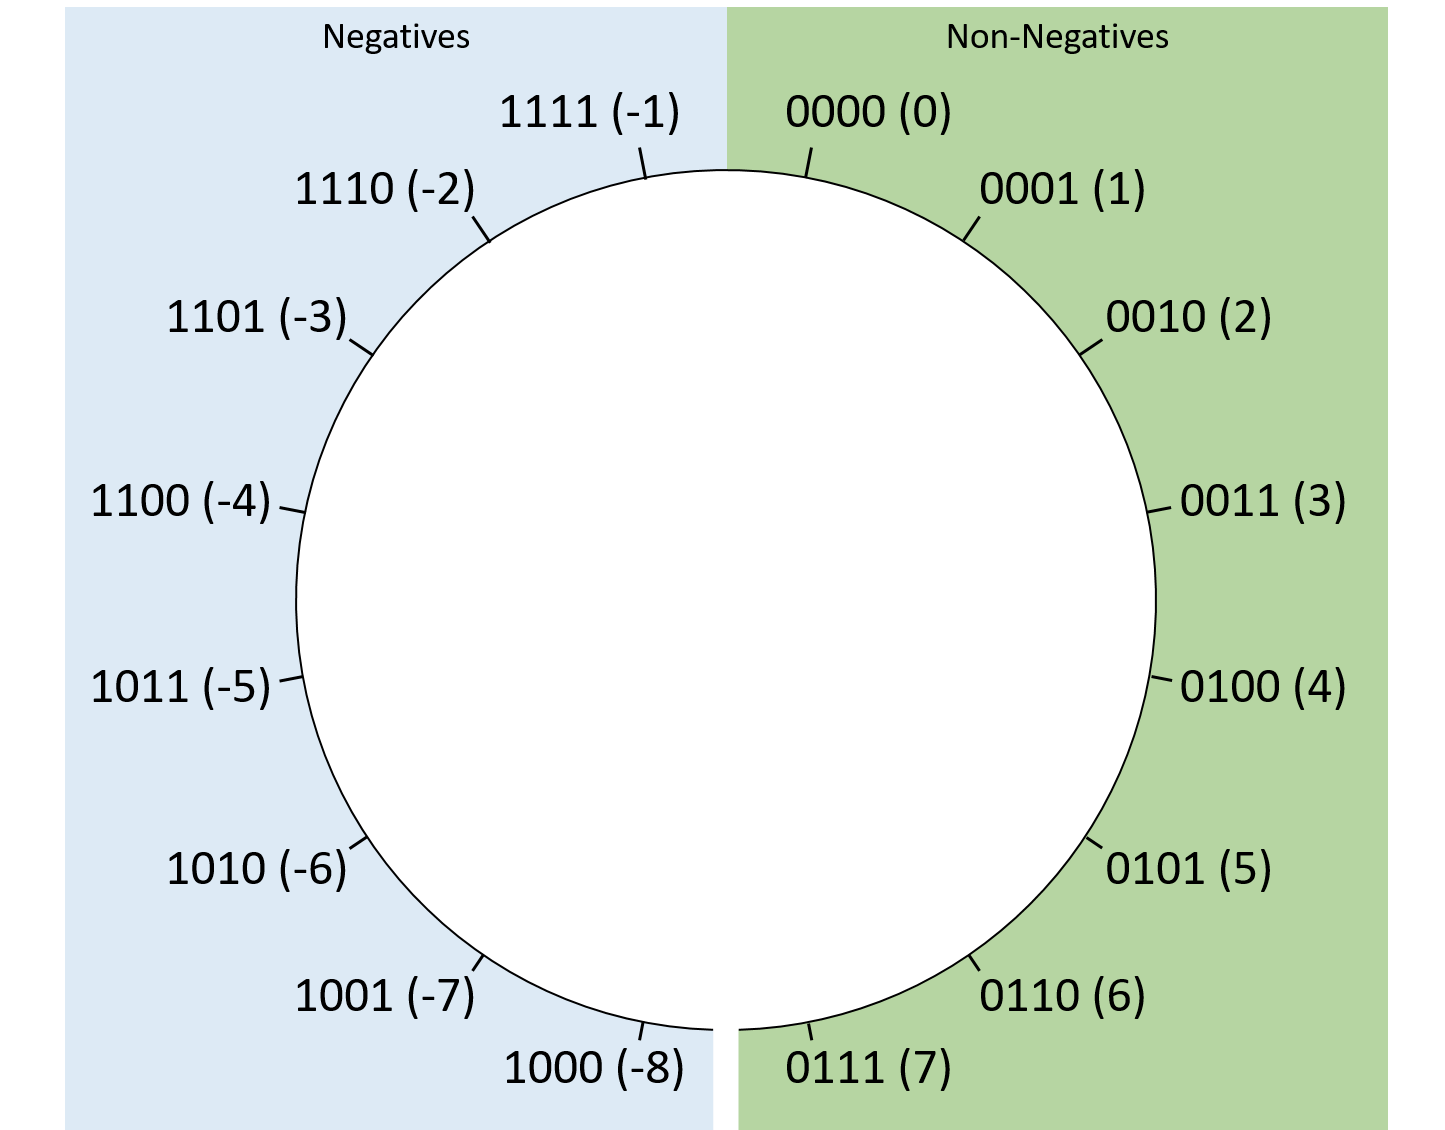
\includegraphics[width=0.41\textwidth]{circle-twoscomplement.png} % Replace 'path_to_image.png' with the actual path to your image file
			\caption*{Circular representation of two's complement}
		\end{wrapfigure}
		
		In two's complement arithmetic, a circular graphical representation can be used to illustrate the addition and subtraction of numbers:
		\begin{itemize}
			\item[-] Moving \textbf{clockwise} from 0 represents the \textit{addition} of positive numbers.
			\item[-] Moving \textbf{counterclockwise} represents the \textit{subtraction} of positive numbers.
			\item[-] Crossing the line where the sign changes indicates a \textit{change of sign} from positive to negative or vice versa.
			\item[] \textbf{Examples:}
			      \begin{itemize}
			      	\item[] The addition of two positive numbers, such as \(2 + 3\), is shown by moving clockwise from 0 to 2 and then moving 3 more steps clockwise, resulting in 5.
			      	\item[] The subtraction of a smaller number from a larger number, such as \(5 - 3\), is shown by moving clockwise from 0 to 5 and then moving 3 steps counterclockwise, resulting in 2.  
			      \end{itemize}
		\end{itemize}
		
		\subsection{Addition and Subtraction}
		\subsection{Addition}
		Given two \(n\)-bit numbers \(A\) and \(B\), their sum in two's complement arithmetic is obtained by directly adding them together as binary numbers:
		\begin{equation}
			\text{Sum} = A + B
		\end{equation}
		If there is an overflow, i.e., a carry out of the most significant bit (MSB), it is discarded. The result is also represented in \(n\) bits.
		
		\subsection{Subtraction}
		To subtract one \(n\)-bit number \(B\) from another \(A\) using two's complement arithmetic, convert \(B\) to its two's complement and then add it to \(A\):
		\begin{enumerate}
			\item Find the two's complement of \(B\), denoted as \(\bar{B}\), by inverting all the bits of \(B\) and adding \(1\).
			\item Add \(A\) to the two's complement of \(B\):
			      \begin{equation}
			      	\text{Difference} = A + \bar{B}
			      \end{equation}
		\end{enumerate}
		As with addition, discard any overflow from the MSB.
		
		
		\section{Binary Multiplication}
		
		\begin{proof}[Proof]
			Let $X$ and $Y$ be two numbers, then their product can be represented as:
			\begin{align*}
				X \cdot Y & = X \cdot \left( -Y_{n-1} \cdot 2^{n-1} + X \sum_{i=0}^{n-2} Y_i \cdot 2^i \right)                                                                \\
				          & = -X \cdot Y_{n-1} \cdot 2^{n-1} + X \sum_{i=0}^{n-2} Y_i \cdot 2^i                                                                               \\
				          & = -Y_{n-1} \cdot X \cdot 2^{n-1} + Y_{n-2} \cdot X \cdot 2^{n-2} + \ldots + Y_2 \cdot X \cdot 2^2 + Y_1 \cdot X \cdot 2^1 + Y_0 \cdot X \cdot 2^0 
			\end{align*}
		\end{proof}
		    
		  
		
		\newpage
		Binary multiplication operates similarly to decimal multiplication but is performed bit by bit. Here is a clearer example illustrating the multiplication of two binary numbers:
		
		\begin{align*}
			  & \text{Multiplicand} & 1101           & \quad & \text{(This is the number to be multiplied)}                              \\
			  & \text{Multiplier}   & \times \; 0011 &       & \text{(This number multiplies the multiplicand)}                          \\
			\cline{2-4}
			  &                     & 1101           &       & \text{(Multiply by 1, the least significant bit of the multiplier)}       \\
			  & +                   & 11010          &       & \text{(Multiply by 1, add one zero to the right, (left shift, $<<1$))}    \\
			  & +                   & 000000         &       & \text{(Multiply by 0, add two zeros to the right, (left shift, $<<2$))}   \\
			  & +                   & 0000000        &       & \text{(Multiply by 0, add three zeros to the right, (left shift, $<<3$))} \\
			\cline{2-4}
			  &                     & 100111         &       & \text{(Sum of the partial products)}                                      
		\end{align*}
		
		
		
		
		\chapter{Number Systems (Part III)}
		\section{Fixed-Point
		Number Representation}  
		
		Let \(x\) be an integer :
		$x  = x_{int} + x_{fr}$, with $x_{int}$ the integer part and $x_{fr}$ the fractional part.
		
		Let \( X \) be a digit-vector:
		
		\[ X = (X_{m-1} X_{m-2} \dots X_1 X_0 \; . \;  X_{-1} X_{-2} \dots X_{-f}) \]
		
		where
		\begin{itemize}
			\item[] \( X_{m-1} \) to \( X_0 \) represent the integer component
			\item[] \( X_{-1} \) to \( X_{-f} \) represent the fractional component
			\item[] The dot (.) represents the radix point (assumed to be fixed)
		\end{itemize}
		\vskip 0.5cm
		For unsigned numbers:
		\[ x = \sum_{i=-f}^{m-1} X_i \cdot 2^i \]
		
		\vskip 0.5cm
		For signed numbers in two's complement:
		
		\[ x = -X_{m-1} \cdot 2^{m-1} + \sum_{i=-f}^{m-2} X_i \cdot 2^i \]
		
		\newpage
		\subsection{Examples of Fixed-Point Numbers}
		\subsubsection{ Decimal Numbers}
		
		\begin{itemize}
			\item[] Decimal number system with \( m = 5, f = 5 \)
			\item[] Example decimal digit vector
			      \[
			      	x = (10077.01690)
			      \]
			      \[
			      	x = 1 \cdot 10^4 + 7 \cdot 10^1 + 7 \cdot 10^0 + 1 \cdot 10^{-2} + 6 \cdot 10^{-3} + 9 \cdot 10^{-4}
			      \]
			      \[
			      	= 10000 + 70 + 7 + 0.01 + 0.006 + 0.0009
			      \]
			      \[
			      	= 10077.0169
			      \]
			\item[] Most negative (min):
			      \[
			      	x_{\text{min}} = -99999.99999 = \frac{-9999999999}{10^5}
			      \]
			\item[] Largest number (max, positive):
			      \[
			      	x_{\text{max}} = +99999.99999 = \frac{+9999999999}{10^5}
			      \]
		\end{itemize}
		
		\subsubsection{Unsigned Binary Numbers}
		
		\begin{itemize}
			\item[] Unsigned with \( m = 3, f = 4 \)
			\item[] Example binary digit vector
			      \[
			      	X = 1 \cdot 2^2 + 0 \cdot 2^1 + 1 \cdot 2^0 + 0 \cdot 2^{-1} + 1 \cdot 2^{-2} + 1 \cdot 2^{-3} + 1 \cdot 2^{-4} = 5.4375 \]
			      	
			      	\item[] Smallest number (min):
			      	\[
			      		x_{\text{min}} = 000.0000_2 = 0
			      	\]
			      	\item[] Largest number (max):
			      	\[
			      		x_{\text{max}} = 111.1111_2 = 7 + \frac{15}{16} = 7,9375
			      	\]
			      	\end{itemize}
			      	    
			      	\subsubsection{Sign-and-Magnitude Binary Numbers}
			      	\begin{itemize}
			      		\item[] Sign-and-magnitude with \( m = 5, f = 3 \)
			      		\item[] Example binary digit vector
			      		      \[
			      		      	X = (-1)^{1} \cdot (1 \cdot 2^2 + 0 \cdot 2^1 + 1 \cdot 2^0 + 1 \cdot 2^{-1} + 1 \cdot 2^{-2} + 0 \cdot 2^{-3}) = -5.75
			      		      \]
			      		\item[] Most negative number (min):
			      		      \[
			      		      	x_{\text{min}} = 1 1111.111_2 = -15 + \frac{7}{8} = -15.875
			      		      \]
			      		\item[] Largest number (max, positive):
			      		      \[
			      		      	x_{\text{max}} = 0 1111.111_2 = 15 + \frac{7}{8} = 15.875
			      		      \]
			      	\end{itemize}
			      	      
			      	\section{Concepts of
			      	Finite Precision Math}
			      	\subsection{Precision}
			      	Let \( X \) be a digit-vector:
			      	\[ X = (X_{m-1} X_{m-2} \dots X_1 X_0 \; . \;  X_{-1} X_{-2} \dots X_{-f}) \]
			      	
			      	Precision is the maximum number of non zero bits.
			      	$$Precision(x) = m + f$$ with \(m\) the number of bits for the integer part and \(f\) the number of bits for the fractional part.
			      	
			      	\subsection{Resolution}
			      	Resolution is the smallest non-zero number that can be represented.
			      	
			      	$$Resolution(x) = 2^{-f}$$
			      	
			      	
			      	\subsection{Range}
			      	The range of a fixed-point number is the difference between the largest and smallest numbers that can be represented.
			      	
			      	\[Range(x) = x_{\text{max}} - x_{\text{min}}\]
			      	\newblock
			      	\newline
			      	In two's complement, the range is given by:
			      	\[ Range(x) = \displaystyle\sum_{i=-f}^{m-2} 2^i - \left( -2^{m-1} \right)\]
			      	
			      	\subsection{Accuracy}
			      	Accuracy is the maximum difference between a real value and the represented value.
			      	
			      	$$Accuracy(x) = \frac{Resolution(x)}{2}$$
			      	
			      	\subsection{Dynamic Range}
			      	The dynamic range is the ratio of the largest and the smallest positive number that can be represented.
			      	
			      	$$Dynamic \; Range(x) = \frac{|x_{max}|}{|x_{\text{positive, nonzero min}}|}$$
			      	
			      	\textit{In two's complement :}
			      	$$Dynamic \; Range(x) = \frac{2^{m-1}}{2^{-f}} = 2^{m-1+f}$$
			      	
			      	\section{Floating-Point Number Representation}
			      	\textit{Personal Remark. Please take the time to really understand this part. It is crucial for the understanding of the rest of the course. Take some time to understand the vocabulary and its meaning.}\newline
			      	\vskip 0.5cm
			      	A real number that is exactly representable in a computer is called a \textbf{floating-point number}. 
			      	\subsection{Significand, Base, Exponent}
			      	A floating-point number consits of a \textbf{significand} (or mantissa), a \textbf{base} (or radix), and an \textbf{exponent}.
			      	\begin{itemize}
			      		\item[] the signed \textit{significand} (also called \textit{mantissa}) \( M^* \)
			      		\item[] the signed \textit{exponent} \( E \)
			      	\end{itemize}
			      	
			      	where \( b \) is a constant called the \textit{base}
			      	
			      	\[ x = M^* \times b^E \]
			      	
			      	This reminds us of the usual scientific notation, base 10:
			      	\begin{itemize}
			      		\item[] \( +35200 = +3.52 \times 10^4 \) (Coefficient)
			      		\item[] \( -0.099 = -9.9 \times 10^{-2} \) (Exponent)
			      	\end{itemize}
			      	
			      	\subsection{Benefits }
			      	\begin{enumerate}
			      		\item \textit{Consider 32-bit two's complement signed integers}
			      		          
			      		      The dynamic range for a 32-bit two's complement signed integer can be expressed as:
			      		      \begin{equation*}
			      		      	\text{Dynamic Range}_1 (x) = \frac{\lvert x \rvert_{\text{max}}}{\lvert x_{\text{positive, nonzero}} \rvert_{\text{min}}} = \frac{\lvert -2^{32-1} \rvert}{2^0} = 2^{31} \approx 2 \cdot 10^9
			      		      \end{equation*}
			      		          
			      		\item \textit{Consider 32-bit floating-point number, with 24-bits significand and 8-bit exponent in Sign and Magnitude}
			      		             
			      		      {$\text{Dynamic Range}_2 (x) = \frac{\lvert x \rvert_{\text{max}}}{\lvert x_{\text{positive, nonzero}} \rvert_{\text{min}}}$ $$= \frac{(2^{23} - 1) \cdot 2^{(2^{8-1}) - 1}}{2^{-128}} = \frac{(2^{23} - 1) \cdot 2^{127}}{2^{-128}} = (2^{23} - 1) \cdot 2^{255} \approx 5 \cdot 10^{83}$$}
			      		      
			      		          
			      		\item \textit{Dynamic range increase}
			      		          
			      		      Comparing the two dynamic ranges:
			      		      \begin{equation*}
			      		      	\frac{\text{Dynamic Range}_2 (x)}{\text{Dynamic Range}_1 (x)} \approx 10^{74}
			      		      \end{equation*}
			      	\end{enumerate}
			      	\newpage
			      	
			      	
			      	\begin{enumerate}
			      		
			      		\item \textit{Consider a fixed-point number with 8 fractional bits}
			      		      \begin{equation*}
			      		      	\text{Resolution}_1(x) = 2^{-8}
			      		      \end{equation*}
			      		          
			      		\item \textit{Consider 32-bit floating-point number, with 24-bits significand in sign-and-magnitude and 8-bit exponent in two's complement}
			      		      \begin{equation*}
			      		      	\text{Resolution}_2(x) = 2^0 \cdot 2^{-2^(8-1)} = 2^{-2^7} = 2^{-128}
			      		      \end{equation*}
			      		          
			      		\item \textit{Improved resolution}
			      		      \begin{equation*}
			      		      	\frac{\text{Resolution}_2(x)}{\text{Resolution}_1(x)} = \frac{2^{-128}}{2^{-8}} = 2^{-120}
			      		      \end{equation*}
			      	\end{enumerate}
			      	
			      	
			      	    
			      	\subsection{Representation}
			      	\begin{itemize}
			      		\item[] We will be focusing on the following digit-vector:
			      		      \[
			      		      	X = (\underbrace{S}_{\text{\color{purple}Sign}}E_{m-1}E_{m-2}\dots E_1E_0\underbrace{M_{n-1}M_{n-2}\dots M_0}_{\text{\color{purple}Magnitude}})
			      		      \]
			      		      
			      		      
			      		      The floating-point representation becomes
			      		      \[
			      		      	x = (-1)^s \times M \times b^E
			      		      \]
			      		      where \( s \in \{0, 1\} \) is the \textbf{sign}, and \( M \) is the \textbf{magnitude} of the signed significant
			      		      \vskip 0.5cm
			      		      \textbf{In the rest of the lecture, we assume significand is represented in sign-and-magnitude.}
			      	\end{itemize}
			      	
			      	
			      	\subsubsection[short]{Normalization}
			      	The goal of normalization is to represent the number such that the magnitude (\(M\)) is within the range \(1 \leq M < 2\). This means that the leading digit before the binary point is always 1. Here are examples to demonstrate this process:
			      	
			      	\begin{itemize}
			      		\item[] \textbf{Positive Example}:
			      		      \begin{itemize}
			      		      	\item[] Given: \( +1010.1000_2 \)
			      		      	\item[] Normalize: \( +1.1010_2 \times 2^3 \)
			      		      	\item[] Decimal Conversion: \( 1.3125 \times 8 = 10.5 \)
			      		      	\item[] Explanation: The binary number \(1010.1000_2\) is normalized by shifting the binary point such that the first digit is 1, and adjusting the exponent (\(2^3\)) accordingly. The equivalent decimal number is \(10.5\).
			      		      \end{itemize}
			      		      \newpage
			      		\item[] \textbf{Negative Example}:
			      		      \begin{itemize}
			      		      	\item[] Given: \( -(0.00000011)_2 \)
			      		      	\item[] Normalize: \( -1.1_2 \times 2^{-7} \)
			      		      	\item[] Decimal Conversion: \( -(1.5)_{10} \times 2^{-7} = -0.01171875 \)
			      		      	\item[] Explanation: The binary number \(0.00000011_2\) is normalized by shifting the binary point to get a leading 1, and adjusting the exponent (\(2^{-7}\)) to reflect the shift. The equivalent decimal number is \(-0.01171875\).
			      		      \end{itemize}
			      	\end{itemize}
			      	    
			      	\subsubsection{Why Normalize?}
			      	    
			      	Normalization removes redundancy from floating-point representation, making it unique. Consider these examples to understand the redundancy in non-normalized representations:
			      	
			      	\[
			      		\begin{aligned}
			      			  & + (1010)_2 \times 2^{-2} = 10 \times 2^{-2} = 2.5; \\
			      			  & + (1.01)_2 \times 2^{1} = 1.25 \times 2^{1} = 2.5; \\
			      			  & + (0101)_2 \times 2^{-1} = 5 \times 2^{-1}  = 2.5; \\
			      		\end{aligned}
			      	\]
			      	
			      	    
			      	In these cases, different representations lead to the same decimal value, illustrating redundancy. Normalization ensures that each number has a unique floating-point representation. 
			      	\vskip 0.5cm
			      	\textbf{Conclusion}: Floating-point representation is \textcolor{red}{redundant unless it is normalized}. By normalizing, we ensure a unique and efficient representation for computational purposes.
			      	\vskip 0.5cm
			      	In normalized floating-point representation, the leading digit is always 1 and is omitted as a hidden bit to save space, with the remaining digits representing the fraction part of the significand :
			      	\begin{itemize}
			      		\item[] \( +(101.001)_2 \times 2^{-4} \Rightarrow +(1.01001)_2 \times 2^{-2} \Rightarrow +(.01001)_2 \times 2^{-2} \)
			      	\end{itemize}
			      	
			      	
			      	
			      	
			      	\newpage
			      	\subsection{Biased Representation}
			      	
			      	Given a binary number with $n$ bits, the value of the biased representation can be calculated as follows:
			      	
			      	\[
			      		x = (\sum_{i=0}^{n-1} X_i \cdot 2^i) - B
			      	\]
			      	
			      	Where $X_i$ represents the $i^{th}$ bit of the binary number (starting from 0 for the least significant bit), and $B$ is the bias, which is calculated by:
			      	
			      	\[
			      		B = 2^{(n-1)} - 1
			      	\]
			      	
			      	
			      	The exponent thus becomes : 
			      	\[ e = (\sum_{i=0}^{n-1} E_i \cdot 2^i) - (2^{(n-1)} - 1) \]
			      	
			      	For instance, with a 3-bit binary number, the bias $B$ is $2^{(3-1)} - 1 = 3$. Therefore, the biased representation maps binary numbers to the integer range from $-B$ to $2^n - 1 - B$.
			      	
			      	\subsubsection{Example}
			      	
			      	For a 3-bit binary number, the biased representations would be:
			      	
			      	\begin{center}
			      		\begin{tabular}{ccc}
			      			\textbf{Decimal} & \textbf{Binary} & \textbf{Biased Decimal} \\
			      			\hline
			      			7                & 111             & 4                       \\
			      			6                & 110             & 3                       \\
			      			5                & 101             & 2                       \\
			      			4                & 100             & 1                       \\
			      			3                & 011             & 0                       \\
			      			2                & 010             & -1                      \\
			      			1                & 001             & -2                      \\
			      			0                & 000             & -3                      \\
			      		\end{tabular}
			      	\end{center}
			      	
			      	Note that the minimum exponent in the biased representation is zero so that the representation of FP zero value is all zeros (zero sign, exponent, and mantissa).
			      	
			      	\newpage
			      	\section*{Summary of the Floating-Point Representation}
			      	Let the binary vector : 
			      	\[ X = (S E_{m-1}E_{m-2}\dots E_1E_0 \; . \; M_{n-1}M_{n-2}\dots M_0) \]
			      	
			      	\begin{itemize}
			      		\item[] $(m)$-bit exponent
			      		      \begin{itemize}
			      		      	\item[-] Biased, $B = 2^{m-1} - 1$
			      		      \end{itemize}
			      		\item[] $(n + 1)$-bit significand
			      		      \begin{itemize}
			      		      	\item[-] Sign-and-magnitude
			      		      	\item[-] Normalized, one hidden bit
			      		      \end{itemize}
			      		      
			      	\end{itemize}
			      	
			      	\[
			      		x = (-1)^S \times \left(1 + \sum_{i=1}^{n} M_{n-i}2^{-i} \right) \times 2^{\left(\sum_{j=0}^{m-1} E_j2^j\right) - (2^{m-1} - 1)}
			      	\]
			      	\subsection{Rounding}
			      	\begin{itemize}
			      		\item[] The result of a floating-point operation is a real number that, to be represented exactly, might require a significand with an infinite number of digits.
			      		      \begin{itemize}
			      		      	\item[] For a representation close to the exact result, we perform \textbf{rounding}.
			      		      \end{itemize}
			      		\item[] Consider the real number \( x_{\text{real}} \) and the consecutive floating-point numbers \( F_1 \) and \( F_2 \), such that \( F_1 \leq x_{\text{real}} \leq F_2 \).
			      		      \begin{itemize}
			      		      	\item[] We can perform several types of rounding:
			      		      	      \begin{itemize}
			      		      	      	\item[] Round to nearest (tie to even)
			      		      	      	\item[] Round towards zero (truncation)
			      		      	      	\item[] Round towards plus or towards minus infinity
			      		      	      \end{itemize}
			      		      \end{itemize}
			      	\end{itemize}
			      	\begin{itemize}
			      		\item[-] Round to nearest (tie to even)
			      		      \[ R_{\text{near}}(x_{\text{real}}) = 
			      		      	\begin{cases} 
			      		      		F_1,                   & \text{if } |x_{\text{real}} - F_1| < |x_{\text{real}} - F_2| \\
			      		      		F_2,                   & \text{if } |x_{\text{real}} - F_1| > |x_{\text{real}} - F_2| \\
			      		      		\text{even}(F_1, F_2), & \text{if } |x_{\text{real}} - F_1| = |x_{\text{real}} - F_2| 
			      		      	\end{cases}
			      		      \]
			      		          
			      		\item[-] Round towards zero (truncation)
			      		      \[ R_{\text{zero}}(x_{\text{real}}) = 
			      		      	\begin{cases} 
			      		      		F_1, & \text{if } x_{\text{real}} \geq 0 \\
			      		      		F_2, & \text{if } x_{\text{real}} < 0    
			      		      	\end{cases}
			      		      \]
			      		          
			      		\item[-] Round towards plus or minus (negative) infinity
			      		      \[ R_{\text{pinf}}(x_{\text{real}}) = F_2 \]
			      		      \[ R_{\text{ninf}}(x_{\text{real}}) = F_1 \]
			      	\end{itemize}
			      	
			      	\section*{Examples of Rounding Methods}
			      	
			      	Let's consider \( x_{\text{real}} = 2.5 \), \( F_1 = 2 \), and \( F_2 = 3 \) for our examples.
			      	
			      	\subsection*{Round to nearest (tie to even)}
			      	\[ R_{\text{near}}(2.5) = \text{even}(2, 3) = 2 \]
			      	Since both \( F_1 \) and \( F_2 \) are equidistant from \( x_{\text{real}} \), we choose the even number which is \( 2 \).
			      	
			      	\subsection*{Round towards zero (truncation)}
			      	\[ R_{\text{zero}}(2.5) = 2 \]
			      	Since \( x_{\text{real}} \) is positive, we round towards zero, resulting in \( F_1 \).
			      	
			      	\subsection*{Round towards plus infinity}
			      	\[ R_{\text{pinf}}(2.5) = 3 \]
			      	When rounding towards plus infinity, we choose \( F_2 \).
			      	
			      	\subsection*{Round towards minus infinity}
			      	\[ R_{\text{ninf}}(2.5) = 2 \]
			      	When rounding towards minus infinity, we choose \( F_1 \).
			      	
			      	Now let's consider a negative value \( x_{\text{real}} = -2.5 \), \( F_1 = -3 \), and \( F_2 = -2 \).
			      	
			      	\subsection*{Round towards zero (truncation) for negative value}
			      	\[ R_{\text{zero}}(-2.5) = -2 \]
			      	Since \( x_{\text{real}} \) is negative, we round towards zero, resulting in \( F_2 \).
			      	
			      	\subsection*{Round towards plus infinity for negative value}
			      	\[ R_{\text{pinf}}(-2.5) = -2 \]
			      	When rounding towards plus infinity for a negative number, we choose the larger number, which is \( F_2 \).
			      	
			      	\subsection*{Round towards minus infinity for negative value}
			      	\[ R_{\text{ninf}}(-2.5) = -3 \]
			      	When rounding towards minus infinity for a negative number, we choose the smaller number, which is \( F_1 \).
			      	
			      	
			      	\newpage 
			      	\section{IEEE 754 Standard}
			      	\section*{FP Format in IEEE 754}
			      	
			      	Exactly what we described:
			      	\begin{itemize}
			      		\item[] \( (n + 1) \)-bit significand
			      		      \begin{itemize}
			      		      	\item Sign-and-magnitude
			      		      	\item Normalized, one hidden bit
			      		      \end{itemize}
			      		\item[] \( m \)-bit exponent
			      		      \begin{itemize}
			      		      	\item Biased, \( B = 2^{m-1} - 1 \)
			      		      \end{itemize}
			      	\end{itemize}
			      	
			      	Let \( X \) a digit-vector represented as:
			      	\[ X = (S E_{m-1} E_{m-2} \ldots E_1 E_0 . M_{n-1} M_{n-2} \ldots M_1 M_0) \]
			      	
			      	\underline{Basic and extended formats:}
			      	\begin{itemize}
			      		\item[+] Basic formats:
			      		      \begin{itemize}
			      		      	\item Single precision (32 bits)
			      		      	      \begin{itemize}
			      		      	      	\item Sign \( S \): 1 bit
			      		      	      	\item Exponent \( E \): 8 bits
			      		      	      	\item Fraction \( F \): 23 bits
			      		      	      \end{itemize}
			      		      	\item Double precision (64 bits)
			      		      	      \begin{itemize}
			      		      	      	\item Sign \( S \): 1 bit
			      		      	      	\item Exponent \( E \): 11 bits
			      		      	      	\item Fraction \( F \): 52 bits
			      		      	      \end{itemize}
			      		      \end{itemize}
			      		\item[+] Default round to nearest (ties to even)
			      	\end{itemize}
			      	
			      	\newpage
			      	\subsection{Special Values}
			      	The IEEE 754 standard defines special values with unique bit patterns:
			      	
			      	\begin{description}
			      		\item[Floating-point zero:] is represented by all zeros in both the exponent and the significand fields.
			      		\begin{align*}
			      			\text{Positive zero: } & 0 \quad 00000000 \quad 00000000000000000000000 \\
			      			\text{Negative zero: } & 1 \quad 00000000 \quad 00000000000000000000000 
			      		\end{align*}
			      		The most significant bit (the sign bit) differentiates between positive and negative zero.
			      		
			      		\item[Positive and negative infinity:] are represented by all ones in the exponent field and all zeros in the significand field.
			      		\begin{align*}
			      			\text{Positive infinity: } & 0 \quad 11111111 \quad 00000000000000000000000 \\
			      			\text{Negative infinity: } & 1 \quad 11111111 \quad 00000000000000000000000 
			      		\end{align*}
			      		
			      		\item[NaN (Not a Number):] is represented by all ones in the exponent field and a non-zero significand field.
			      		\begin{align*}
			      			\text{NaN (example): } & - \quad 11111111 \quad 10000000000000000000000 
			      		\end{align*}
			      		NaN values represent indeterminate or undefined results, such as the square root of a negative number. The sign bit can be either 0 or 1, but the significand must not be all zeros.
			      	\end{description}
			      	
			      	\subsection{Overflow, underflow, and others}
			      	\begin{description}
			      		\item[Overflow:] Occurs when the rounded value is too large to be represented by the floating-point format.
			      		\begin{itemize}
			      			\item The result is set to positive or negative infinity, depending on the sign.
			      		\end{itemize}
			      		    
			      		\item[Underflow:] Happens when the rounded value is too small to be represented.
			      		\begin{itemize}
			      			\item Typically, the result is set to a denormalized number or zero.
			      		\end{itemize}
			      		    
			      		\item[Division by zero:] Occurs when a finite non-zero number is divided by zero.
			      		\begin{itemize}
			      			\item The result is set to positive or negative infinity, based on the sign of the numerator.
			      		\end{itemize}
			      		    
			      		\item[Inexact result:] Occurs when the result of an operation is not an exact floating-point number.
			      		\begin{itemize}
			      			\item The result is rounded to the nearest representable value.
			      		\end{itemize}
			      		    
			      		\item[Invalid:] This flag is set when the result of an operation is not a real number (NaN).
			      		\begin{itemize}
			      			\item Examples include the square root of a negative number or the indeterminate form 0/0.
			      		\end{itemize}
			      	\end{description}
			      	
			      	\section*{IEEE 754}
			      	\subsection*{Example: Converting single-precision FP to decimal}
			      	
			      	Find the decimal equivalent of
			      	\[ X = (1\ 01111100\ 01000000000000000000000) \]
			      	
			      	Solution:
			      	\begin{itemize}
			      		\item[-] Sign \( S = 1 \), hence negative.
			      		\item[-] Exponent \( E = 01111100 \) represents the biased exponent. To find the actual exponent:
			      		      \[ E_{\text{actual}} = 124 - (2^7 - 1) = 124 - 127 = -3 \]
			      		\item[-] Mantissa (including the hidden bit) \( M = 1.01 \) in binary represents:
			      		      \[ M = 1 + 2^{-2} = 1.25 \]
			      		\item[-] Result:
			      		      \[ x = -1.25 \times 2^{-3} = -0.15625 \]
			      	\end{itemize}
			      	
			      	\subsection*{Example: Converting decimal to single-precision FP}
			      	
			      	Find the single-precision FP equivalent of \( x = -0.8125 \)
			      	
			      	Solution:
			      	\begin{itemize}
			      		\item[-] Sign \( = 1 \), negative.
			      		\item[-] Fraction bits can be obtained using multiplication by 2.
			      		\item[-] Converting \( 0.8125 \) to binary by successive multiplication:
			      		      \begin{align*}
			      		      	0.8125 \times 2 & = 1.625 \rightarrow 1 \\
			      		      	0.625 \times 2  & = 1.25 \rightarrow 1  \\
			      		      	0.25 \times 2   & = 0.5 \rightarrow 0   \\
			      		      	0.5 \times 2    & = 1.0 \rightarrow 1   
			      		      \end{align*}
			      		      Stop when the fractional part becomes zero.
			      		\item[-] Mantissa \( M \) in binary is \( 0.1101 \), normalized is \( 1.101 \times 2^{-1} \).
			      		\item[-] Exponent adjustment:
			      		      \[ E_{\text{actual}} = -1 \]
			      		      \[ E = E_{\text{actual}} + B = -1 + (2^7 - 1) = 126 \]
			      		\item[-] Result:
			      		      \[ X = (1\ 01111110\ 10100000000000000000000) \]
			      	\end{itemize}
			      	
			      	
			      	\chapter{Number Systems (Part IV)}
			      	\section{Fixed-Point Arithmetic}
			      	\subsection{Addition and Subtraction}
			      	
			      	Let \( x \) and \( y \) be two fixed-point numbers with the same number of integer and fractional bits. The sum and difference of \( x \) and \( y \) can be calculated as follows:
			      	$$x + y = x_{int} + y_{int} + x_{fr} + y_{fr}$$ 
			      	$$x - y = x_{int} - y_{int} + x_{fr} - y_{fr}$$
			      	 
			      	\subsection{Multiplication}
			      	 
			      	 
			      	\begin{align*}
			      		\begin{array}{r@{}c@{}l}
			      		       & 010.11                          & \text{\quad Multiplicand}                                                 \\
			      		\times & 011.01                          & \text{\quad Multiplier}                                                   \\ \cline{1-2}
			      		       & 000000                          & \text{\quad First partial product (always zero), sign-extended}           \\ 
			      		+      & \; \; \; \; 001011\phantom{.00} & \text{\quad 1 x multiplicand, sign-extended}                              \\ \cline{1-2}
			      		       & 001011                          & \text{\quad Intermediate result, sign-extended}                           \\ 
			      		+      & \phantom{0}00000\phantom{.0}    & \text{\quad 0 x multiplicand, left-shifted by 1 place and sign-extended}  \\ \cline{1-2}
			      		       & 00001011\phantom{}              & \text{\quad Intermediate result, sign-extended}                           \\ 
			      		+      & \phantom{00}001011\phantom{000} & \text{\quad 1 x multiplicand, left-shifted by 2 places and sign-extended} \\ \cline{1-2}
			      		       & 00010111                        & \text{\quad Intermediate result, sign-extended}                           \\ 
			      		+      & 001011\phantom{00}              & \text{\quad 1 x multiplicand, left-shifted by 3 places and sign-extended} \\ \cline{1-2}
			      		       & 001001111                       & \text{\quad Intermediate result, sign-extended}                           \\ 
			      		+      & 000000\phantom{00}              & \text{\quad 0 x multiplicand, left-shifted by 4 places and sign-extended} \\ \cline{1-2}
			      		       & 001000.1111                     & \text{\quad Result}                                                       \\
			      		\end{array} & \text{\quad convert to fixed-point now}
			      	\end{align*}
			      	
			      	\newpage
			      	\section{In two's complement}
			      	Given two fixed-point numbers $x$ and $y$, the addition or subtraction in two's complement is given by:
			      	\begin{equation}
			      		x \pm y = \left( -X_{(m_x-1)}2^{(m_x-1)} + \sum_{i=-f_x}^{m_x-2} X_i2^i \right) \pm \left( -Y_{(m_y-1)}2^{(m_y-1)} + \sum_{i=-f_y}^{m_y-2} Y_i2^i \right)
			      	\end{equation}
			      	
			      	Where:
			      	\begin{itemize}
			      		\item[] $m_x$ and $m_y$ are the total number of bits for the integer components of $x$ and $y$ respectively.
			      		\item[] $f_x$ and $f_y$ are the number of bits for the fractional components of $x$ and $y$ respectively.
			      		\item[] $X_{(m_x-1)}$ and $Y_{(m_y-1)}$ are the sign bits of $x$ and $y$.
			      		\item[] The largest integer-part exponent is $\max(m_x - 1, m_y - 1)$. Consequently, the number of bits for the resulting integer component is $\max(m_x, m_y) + 1$.
			      		\item[] The smallest fractional-part exponent is $\min(-f_x, -f_y)$. Consequently, the number of bits for the resulting fractional component is $\max(f_x, f_y)$.
			      	\end{itemize}
			      	
			      	
			      	\subsection*{Multiplication in Two's Complement}
			      	\begin{itemize}
			      		\item[] Multiplication on two binary numbers \( x(m_x, f_x) \) and \( y(m_y, f_y) \)
			      		      \begin{equation*}
			      		      	x \cdot y = (x_{\text{int}} + x_{\text{fr}}) \cdot (y_{\text{int}} + y_{\text{fr}})
			      		      \end{equation*}
			      		        
			      		\item[] In two's complement:
			      		      \begin{equation*}
			      		      	x \cdot y = \left( -X_{m_x-1}2^{m_x-1} + \sum_{i=-f_x}^{m_x-2} X_i2^i \right) \cdot \left( -Y_{m_y-1}2^{m_y-1} + \sum_{i=-f_y}^{m_y-2} Y_i2^i \right)
			      		      \end{equation*}
			      		          
			      		\item[] \small The largest integer-part exponent: \( (m_x - 1) + (m_y - 1) \). Consequently: \( m_{xy} = m_x + m_y \)
			      		          
			      		\item[] \small The smallest fractional-part exponent: \( (-f_x) + (-f_y) \). Consequently: \( f_{xy} = f_x + f_y \)
			      		          
			      	\end{itemize}
			      	
			      	\section{Floating-Point Arithmetic}
			      	
			      	    
			      	    
			      	\begin{itemize}
			      		\item[] Let \( x \) and \( y \) be represented as \( (S_x, M_x, E_x) \) and \( (S_y, M_y, E_y) \)
			      		      \begin{itemize}
			      		      	\item[] The significands \( M^* = (-1)^S M \) are normalized
			      		      \end{itemize}
			      		            
			      		\item[] Addition/subtraction result is \( z \), also represented as \( (S_z, M_z, E_z) \):
			      		      \[ z = x \pm y = M^*_x \times 2^{E_x} \pm M^*_y \times 2^{E_y} \]
			      		            
			      		      \begin{itemize}
			      		      	\item[] The significand of the result is also normalized
			      		      	      \[ z = M^*_z \times 2^{E_z} \]
			      		      \end{itemize}
			      	\end{itemize}
			      	    
			      	
			      	\newpage
			      	\begin{itemize}
			      		\item[] \textbf{Four main steps to compute the result of floating-point addition/subtraction:}
			      		      \begin{enumerate}
			      		      	\item \textbf{Add/Subtract significand and set exponent:}
			      		      	      \begin{itemize}
			      		      	      	\item Align the significands by shifting the one with the \textit{smaller} exponent.
			      		      	      	\item Perform addition/subtraction on the aligned significands.
			      		      	      \end{itemize}
			      		      	      \[
			      		      	      	M_z^* = 
			      		      	      	\begin{cases} 
			      		      	      		(M_x^* + (M_y^* \times 2^{(E_y - E_x)})) \times 2^{E_x} & \text{if } E_x \geq E_y \\
			      		      	      		((M_x^* \times 2^{(E_x - E_y)}) + M_y^*) \times 2^{E_y} & \text{if } E_x < E_y    
			      		      	      	\end{cases}
			      		      	      \]
			      		      	      \[
			      		      	      	E_z = \max(E_x, E_y)
			      		      	      \]
			      		      	            
			      		      	\item \textbf{Normalize the result and update the exponent, if required:}
			      		      	      \begin{itemize}
			      		      	      	\item Check if the result's significand is within the normalized range.
			      		      	      	\item If not, shift the significand to the right or left until it is normalized, adjusting the exponent accordingly to maintain the value.
			      		      	      \end{itemize}
			      		      	          
			      		      	\item \textbf{Round the result, normalize, and adjust exponent, if required:}
			      		      	      \begin{itemize}
			      		      	      	\item Apply rounding rules to the significand to fit within the precision limits.
			      		      	      	\item After rounding, if the significand overflows (e.g., carries out during addition), normalize the result again and adjust the exponent.
			      		      	      \end{itemize}
			      		      	          
			      		      	\item \textbf{Set flags for special values, if required:}
			      		      	      \begin{itemize}
			      		      	      	\item Check for overflow or underflow conditions and set flags accordingly.
			      		      	      	\item Identify and mark results that are special values (e.g., infinity, NaN) based on the operation and input values.
			      		      	      \end{itemize}
			      		      \end{enumerate}
			      	\end{itemize}
			      	    
			      	\section*{Step 1: Floating-Point Addition/Subtraction Detailed Algorithm}
			      	\begin{itemize}
			      		\item[] Algorithm steps:
			      		      \begin{itemize}
			      		      	\item Subtract exponents \(d = E_x - E_y\).
			      		      	\item Align significands:
			      		      	      \begin{itemize}
			      		      	      	\item Compare the exponents of the two operands.
			      		      	      	\item Shift right \(d\) positions the significand of the operand with the smallest exponent.
			      		      	      	\item Select as the exponent of the result the largest exponent.
			      		      	      \end{itemize}
			      		      	\item Add/subtract signed significands and produce the sign of the result.
			      		      \end{itemize}
			      	\end{itemize}
			      	    
			      	\begin{table}[h]
			      		\centering
			      		\caption*{Floating-point operations based on the signs of the operands.}
			      		\begin{tabular}{ccc}
			      			\toprule
			      			FP operation & Signs of the operands & Effective operation \\
			      			\midrule
			      			\(+\)        & \(=\)                 & add                 \\
			      			\(+\)        & \(\neq\)              & subtract            \\
			      			\(-\)        & \(=\)                 & subtract            \\
			      			\(-\)        & \(\neq\)              & add                 \\
			      			\bottomrule
			      		\end{tabular}
			      	\end{table}
			      	    
			      	\section*{Step 2: Normalize the Result}
			      	After the initial addition or subtraction, the result may not always be in the normalized form required by floating-point representation standards. Normalization ensures that the significand (mantissa) is within a specific range, usually just below 1 (for binary floating-point numbers, this means the leading bit is just to the right of the decimal point).
			      	    
			      	\begin{itemize}
			      		\item[] Steps for normalization:
			      		      \begin{itemize}
			      		      	\item If the result of the operation causes the significand to exceed its predefined size (overflow), the significand is shifted to the right, and the exponent is increased accordingly.
			      		      	\item Conversely, if the operation results in a significand that's too small (underflow), the significand is shifted to the left, and the exponent is decreased.
			      		      	\item This process ensures that the floating-point number is as close to its true value as possible within the limits of the representation.
			      		      \end{itemize}
			      	\end{itemize}
			      	\section*{Step 3: Round the Result}
			      	
			      	After normalization, the next step is to round the result to fit within the target floating-point format's precision. Rounding is crucial because it affects the accuracy and representation of the result.
			      	    
			      	\begin{itemize}
			      		\item[] Steps for rounding:
			      		      \begin{itemize}
			      		      	\item Evaluate the significand's precision and compare it with the format's limit.
			      		      	\item If the significand exceeds the precision limit, round it according to a rounding rule (e.g., round to nearest, round towards zero, round towards positive/negative infinity).
			      		      	\item Common rounding strategies include:
			      		      	      \begin{itemize}
			      		      	      	\item \textbf{Round to Nearest:} Round to the nearest value, with ties going to the nearest even number.
			      		      	      	\item \textbf{Round Down (Towards Zero):} Always round towards zero, truncating any fractional part.
			      		      	      	\item \textbf{Round Up (Away from Zero):} Always round away from zero, increasing the magnitude of the result.
			      		      	      \end{itemize}
			      		      	\item After rounding, if there's an overflow in the significand (e.g., a carry into a new digit), normalize the result again. This may involve shifting the significand and adjusting the exponent.
			      		      \end{itemize}
			      	\end{itemize}
			      	    
			      	\section*{Step 4: Set Flags for Special Values}
			      	    
			      	The final step in floating-point addition or subtraction involves handling special cases and setting flags accordingly. Special values include infinity, not-a-number (NaN), and potential overflow or underflow conditions.
			      	    
			      	\begin{itemize}
			      		\item[] Handling special values:
			      		      \begin{itemize}
			      		      	\item \textbf{Infinity:} If the result of the operation is too large to be represented in the given floating-point format, set the result to infinity. The sign of infinity depends on the operation and operands.
			      		      	\item \textbf{NaN (Not-a-Number):} If the operation involves invalid operations (e.g., \(0/0\), \(\infty - \infty\)), set the result to NaN. NaN propagates through most floating-point operations.
			      		      	\item \textbf{Overflow:} If the result exceeds the maximum representable value, set an overflow flag. The result is typically set to infinity with the appropriate sign.
			      		      	\item \textbf{Underflow:} If the result is too small to be represented (closer to zero than the smallest representable value), set an underflow flag. The result may be set to zero or the smallest denormalized number, depending on the format and flags.
			      		      \end{itemize}
			      	\end{itemize}
			      	
			      	
			      	\subsection{An Example in Binary}
			      	
			      	Let's add two binary floating-point numbers: $1.01 \times 2^3$ and $1.1 \times 2^2$. Here's how we do it step by step:
			      	
			      	\begin{enumerate}
			      		\item \textbf{Line Up the Dots:} First, we need to align the exponents. We'll adjust the second number to have the same exponent as the first, by increasing its exponent and shifting its significand to the right: 
			      		      \[
			      		      	1.1 \times 2^2 = 0.11 \times 2^3
			      		      \]
			      		      Now, both numbers are $1.01 \times 2^3$ and $0.11 \times 2^3$.
			      		      
			      		\item \textbf{Add Them Up:} With the exponents aligned, we can now add the significands:
			      		      \[
			      		      	1.01 + 0.11 = 10.00
			      		      \]
			      		      The result in binary is $10.00$. Since we're working in binary, $10.00$ is actually $2$ in decimal. 
			      		      
			      		\item \textbf{Make It Look Right:} The result $10.00 \times 2^3$ is already in the correct format, but let's note that if our result was something like $1.000 \times 2^4$, we would need to adjust it to keep it in normalized form.
			      		      
			      		\item \textbf{Round It Off:} Our result doesn't need rounding in this case, but if we had more digits than we could store, we'd round off to the nearest value we could represent.
			      		      
			      		\item \textbf{Check for Special Cases:} There are no special cases here, as our result is a regular binary floating-point number.
			      	\end{enumerate}
			      	
			      	So, our final result is $10.00 \times 2^3$ in binary, which is $8$ in decimal.
			      	
			      	
			      	\chapter{Number Systems (Part V)}
			      	
			      	
			      	
			      	
			      	\begin{text}
			      		This small chapter concludes the Number Systems chapter with a some modern applications of low precision computing.
			      	\end{text}
			      	\section{Low precision computer arithmetic}
			      	
			      	
			      	\begin{itemize}
			      		\item[] AI is taking on an increasingly important role
			      		\item[] Deep Neural Networks (DNNs) are the most widespread
			      		      \begin{itemize}
			      		      	\item[] E.g., Large Language Models (LLM) generate human-like content
			      		      \end{itemize}
			      		\item[] Challenge: exponential size growth
			      		      \begin{itemize}
			      		      	\item[] GPT3 has 175 billion parameters
			      		      \end{itemize}
			      		\item[] Large models mean
			      		      \begin{itemize}
			      		      	\item[] A lot of data, any computations
			      		      	\item[] ...and we want the result quickly!
			      		      	\item[] Luckily, ML models are tolerant to small errors
			      		      \end{itemize}
			      	\end{itemize}
			      	
			      	\section{Challenges and limitations}
			      	\begin{itemize}
			      		\item[] 32-bit or 64-bit floating-point formats
			      		      \begin{itemize}
			      		      	\item[] Arithmetic units are large (many bits $\Rightarrow$ high area, high energy)
			      		      	\item[] We can put fewer units per chip (e.g., less compute power in GPU)
			      		      	      \begin{itemize}
			      		      	      	\item[] Poor arithmetic density (in number of ops / 1mm$^2$)
			      		      	      	\item[] Fewer units, fewer computations
			      		      	      \end{itemize}
			      		      	\item[] The model predictions are accurate, but it takes a long time to compute them
			      		      \end{itemize}
			      		\item[] Fixed-point or integer formats
			      		      \begin{itemize}
			      		      	\item[] Arithmetic units are smaller and faster (approx. 10x area savings)
			      		      	\item[] Better arithmetic density and lower delays
			      		      	\item[] The errors due to limited dynamic range are too significant for most ML models; the accuracy of their predictions suffers
			      		      \end{itemize}
			      		\item[] New number formats are needed: the best of both worlds
			      	\end{itemize}
			      	
			      	
			      	
			      	\section{Block Floating Point}
			      	\section*{Block Floating Point}
			      	
			      	Imagine a block (vector) of binary numbers in FP (Floating Point) format, where each vector element has its own S (Sign), M (Mantissa), and E (Exponent).
			      	
			      	\[
			      		\begin{array}{|c|c|c|}
			      			\hline
			      			S_1    & E_1    & M_1    \\
			      			\hline
			      			S_2    & E_2    & M_2    \\
			      			\hline
			      			\vdots & \vdots & \vdots \\
			      			\hline
			      			S_n    & E_n    & M_n    \\
			      			\hline
			      		\end{array}
			      	\]
			      	
			      	If the exponents in the block are not too different, we could use a single shared exponent per block.
			      	
			      	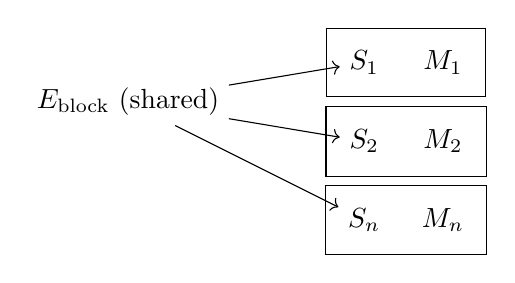
\begin{tikzpicture}
			      		\node (E) at (0,0) {$E_{\text{block}}$ (shared)};
			      		\node (S1) at (3,0.5) {$S_1$};
			      		\node (M1) at (4,0.5) {$M_1$};
			      		\node[draw,fit=(S1) (M1),inner sep=1.65mm] (table1) {}; % Drawing a rectangle around S1 and M1
			      		\node (S2) at (3,-0.5) {$S_2$};
			      		\node (M2) at (4,-0.5) {$M_2$};
			      		\node[draw,fit=(S2) (M2),inner sep=1.75mm] (table1) {}; % Drawing a rectangle around S1 and M1
			      		\node (Sn) at (3,-1.5) {$S_n$};
			      		\node (Mn) at (4,-1.5) {$M_n$};
			      		\node[draw,fit=(Sn) (Mn),inner sep=1.65mm] (table1) {}; % Drawing a rectangle around S1 and M1
			      		
			      		\draw[->] (E) -- (S2);
			      		\draw[->] (E) -- (S1);
			      		\draw[->] (E) -- (Sn);
			      	\end{tikzpicture}
			      	    
			      	
			      	\textit{In BFP with shared Exponent:}
			      	\begin{itemize}
			      		\item[] Find the largest exponent in the block of FP numbers. This will be the shared exponent \( E_{\text{block}} \).
			      		\item[] Calculate the difference \( d_i = E_{\text{block}} - E_i \) between the shared exponent and each of the other exponents \( E_i \) in the block.
			      		\item[] Adjust the mantissa by right-shifting the signed mantissa of each number by \( d_i \). As a result of these adjustments, the mantissa in BFP cannot be normalized, and there is no hidden bit.
			      	\end{itemize}
			      	
			      	\chapter{Digital Logic}
			      	\section{Introduction to Digital Logic Circuits}
			      	The smallest unit of Digital Information is a binary value 1 or 0.
			      	\subsection{The simplest binary logic element}
			      	Similarly, a switch can either be open or closed. 
			      	Let $x$ an input variable.
			      	\begin{itemize}
			      		\item[-] Open ($x=0$) \;
			      		      \begin{tikzpicture}
			      		      	\draw (0,0) -- (2,0);
			      		      	\draw (2,0) -- (2.5,0.5);
			      		      	\draw (3,0) -- (4,0);
			      		      	\filldraw [black] (2,0) circle (2pt);
			      		      	\filldraw [black] (3,0) circle (2pt);
			      		      \end{tikzpicture}
			      		      
			      		\item[-] Closed ($x=1$)
			      		      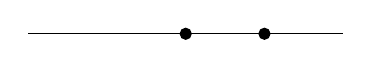
\begin{tikzpicture}
			      		      	\draw (0,0) -- (2,0);
			      		      	\draw (2,0) -- (4,0);
			      		      	\filldraw [black] (2,0) circle (2pt);
			      		      	\filldraw [black] (3,0) circle (2pt);
			      		      	
			      		      \end{tikzpicture}
			      	\end{itemize}
			      	
			      	\vspace*{10px}
			      	
			      	The symbol for a switch controlled by an input variable:
			      	
			      	\vspace*{10px}
			      	\hspace*{130px}
			      	\begin{tikzpicture}
			      		\draw (0,0) -- (1,0) -- (1.5,0) -- (2,0) -- (3,0);
			      		\draw (1.5,0) -- (1.5,-0.5);
			      		    
			      		\draw (1,0) -- (1,1) -- (2,1) -- (2,0);
			      		\node at (1.5,0.5) {$S$};
			      		\node at (1.5,-0.75) {$x$};
			      	\end{tikzpicture}
			      	
			      	
			      	\subsection{The simplest binary logic element}
			      	
			      	
			      	\begin{figure}[htp] % This line sets the wrapfigure environment to place the figure on the right side and occupy half the text width
			      		\centering
			      		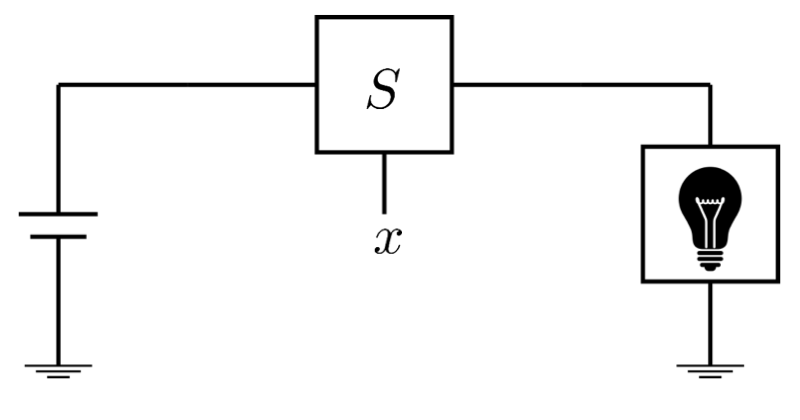
\includegraphics[width=0.41\textwidth]{circuits/6.1.2.png} % Replace 'path_to_image.png' with the actual path to your image file
			      		\caption*{Light controlled by a single switch}
			      	\end{figure}
			      	
			      	
			      	\newpage
			      	\section*{Two-Variable Logic Functions}
			      	\textbf{Series and Parallel Connections}
			      	\newline
			      	\vspace{10px}
			      	\textit{Remark. The choice of symbols is not random $\cdot, +,$ respectively similar to multiplication and addition.}
			      	\vspace{20px}
			      	\begin{figure}[htp] % This line sets the wrapfigure environment to place the figure on the right side and occupy half the text width
			      		\centering
			      		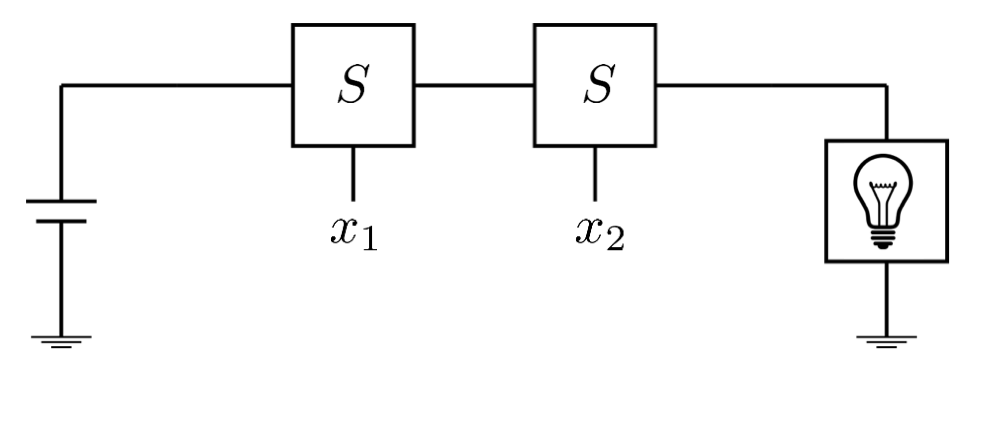
\includegraphics[width=0.41\textwidth]{circuits/6.1.3.png} % Replace 'path_to_image.png' with the actual path to your image file
			      		\caption*{Logic AND function}
			      		\text{$L(x_{1}, x_{2}) = x_{1} \cdot x_{2}$, with $\cdot$ the AND operator}
			      	\end{figure}
			      	
			      	
			      	 
			      	
			      	\begin{figure}[htp] % This line sets the wrapfigure environment to place the figure on the right side and occupy half the text width
			      		\centering
			      		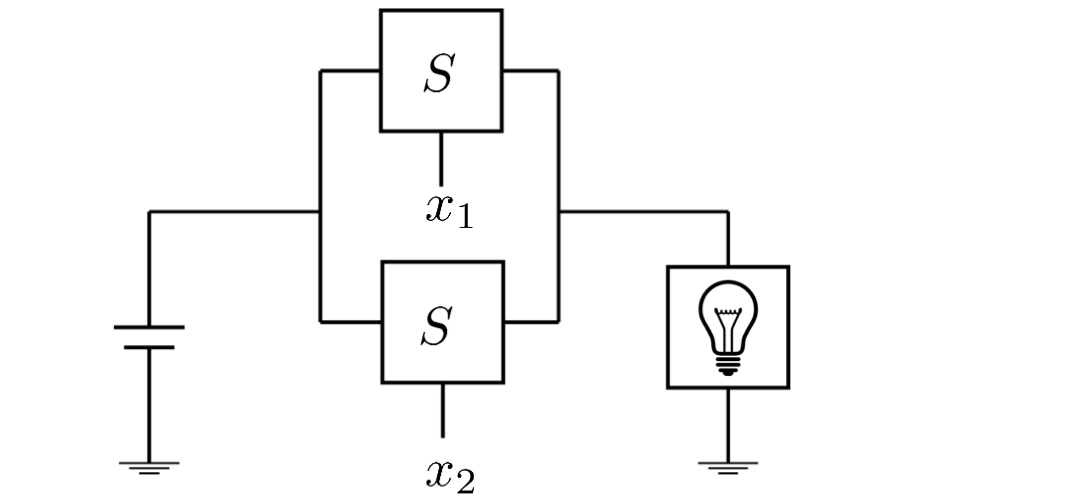
\includegraphics[width=0.5\textwidth]{circuits/6.1.3_2.png} % Replace 'path_to_image.png' with the actual path to your image file
			      		\caption*{Circular representation of two's complement}
			      		\text{$L(x_{1}, x_{2}) = x_{1} + x_{2}$, with $+$ the OR operator}
			      	\end{figure}
			      	
			      	
			      	\begin{figure}[htp] % This line sets the wrapfigure environment to place the figure on the right side and occupy half the text width
			      		\centering
			      		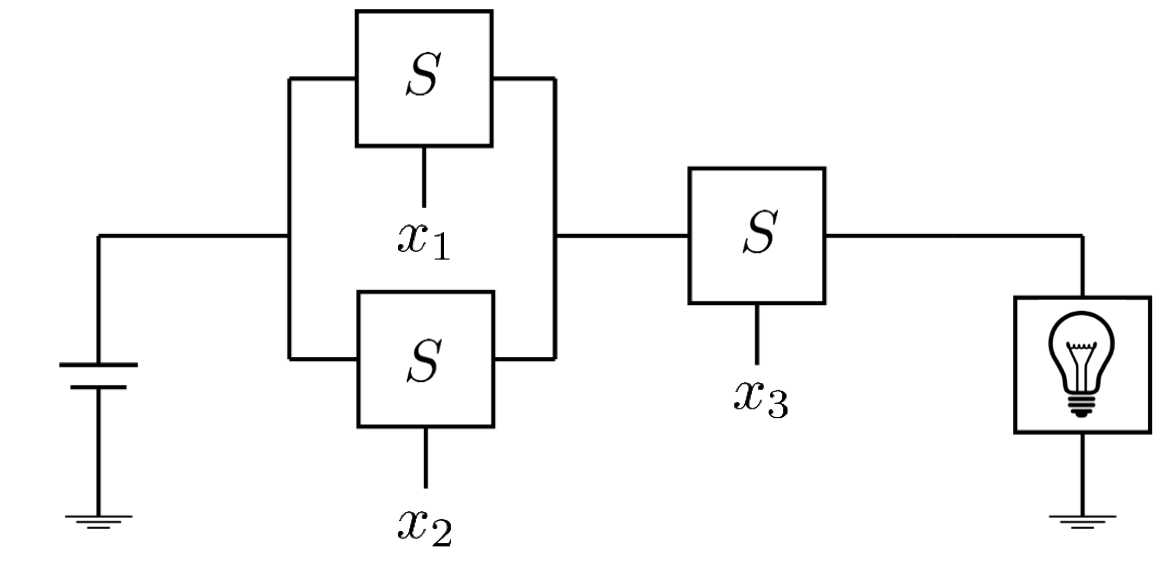
\includegraphics[width=0.5\textwidth]{circuits/6.1.3_3.png} % Replace 'path_to_image.png' with the actual path to your image file
			      		\caption*{A series-parallel connection of three switches}
			      		\text{The corresponding Logic Function is $L(x_{1}, x_{2}, x_{3}) = (x_{1} + x_{2}) \cdot x_{3}$} \newline
			      		\textit{Smaller circuits separated by parentheses}
			      	\end{figure}
			      	
			      	
			      	\begin{figure}[htp]
			      		\centering
			      		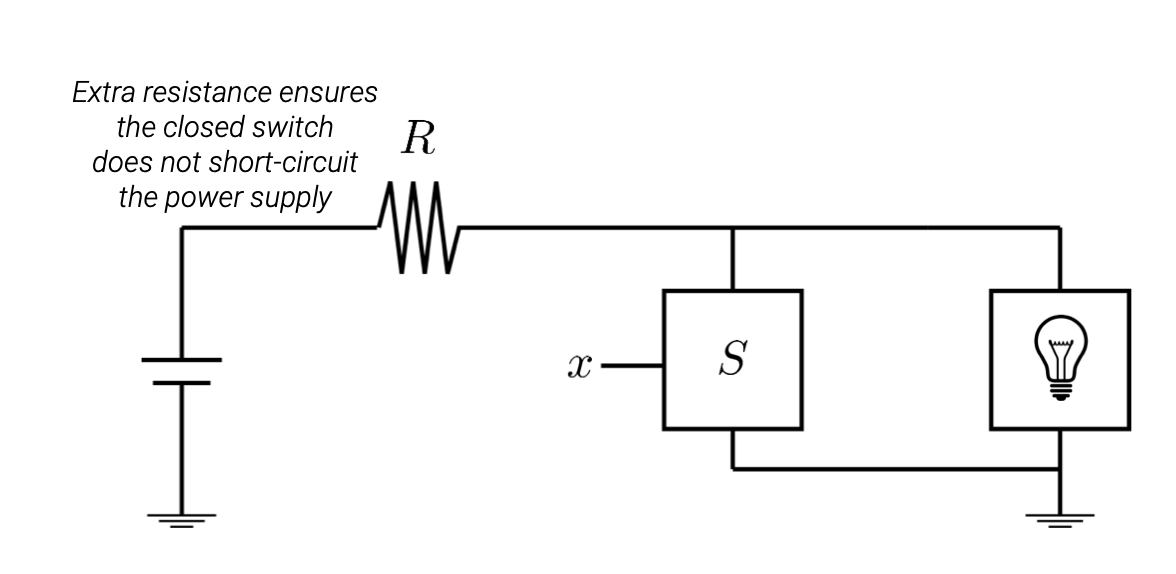
\includegraphics[width=0.5\textwidth]{circuits/6.1.3_4.png} % Adjust the path to your image
			      		\caption*{NOT GATE} % Caption for the figure
			      		\label{fig:notgate} % Label for referencing the figure in the text
			      		\medskip % Adds some vertical space (optional)
			      		\text{The corresponding Logic Function is \(L(x) = \bar{x}\), \textit{ with \(\bar{x}\) the complement of \(x\).}}
			      	\end{figure}
			      	\newpage
			      	\section{Truth Tables}
			      	Logical operations can be defined in the form of a truth table
			      	\begin{itemize}
			      		\item[] AND
			      		      \begin{equation*}
			      		      	L(x_1, x_2) = x_1 \cdot x_2
			      		      \end{equation*}
			      		      where \( L = 1 \) if \( x_1 = 1 \) and \( x_2 = 1 \), \( L = 0 \) otherwise.
			      		            
			      		\item[] OR
			      		      \begin{equation*}
			      		      	L(x_1, x_2) = x_1 + x_2
			      		      \end{equation*}
			      		      where \( L = 1 \) if \( x_1 = 1 \) or \( x_2 = 1 \), or if \( x_1 = x_2 = 1 \), \( L = 0 \) if \( x_1 = x_2 = 0 \).
			      	\end{itemize}
			      	  
			      	\begin{center}
			      		\begin{tabular}{ c c | c | c }
			      			\( x_1 \) & \( x_2 \) & AND & OR \\
			      			\hline
			      			0         & 0         & 0   & 0  \\
			      			0         & 1         & 0   & 1  \\
			      			1         & 0         & 0   & 1  \\
			      			1         & 1         & 1   & 1  \\
			      			      
			      		\end{tabular}
			      	\end{center}
			      	
			      	
			      	\textit{For n logical variables we get $2^n$ rows}.\newline
			      	\vspace*{-10px}
			      	\subsection*{For example :}
			      	\vspace*{-2px}
			      	\begin{itemize}
			      		\item[] AND
			      		      \vspace*{-5px}
			      		      \begin{equation*}
			      		      	L(x_1, x_2, x_3) = x_1 \cdot x_2 \cdot x_3
			      		      \end{equation*}
			      		      where \( L = 1 \) if \( x_1 = x_2 = x_3 = 1 \), \( L = 0 \) otherwise.
			      		      \vspace*{-5px}
			      		\item[] OR
			      		      \begin{equation*}
			      		      	L(x_1, x_2, x_3) = x_1 + x_2 + x_3
			      		      \end{equation*}
			      		      where \( L = 0 \) if \( x_1 = x_2 = x_3 = 0 \), \( L = 1 \) otherwise.
			      	\end{itemize}
			      	
			      	\begin{center}
			      		\begin{tabular}{ c c c | c | c }
			      			
			      			\( x_1 \) & \( x_2 \) & \( x_3 \) & AND & OR \\
			      			\hline
			      			0         & 0         & 0         & 0   & 0  \\
			      			0         & 0         & 1         & 0   & 1  \\
			      			0         & 1         & 0         & 0   & 1  \\
			      			0         & 1         & 1         & 0   & 1  \\
			      			1         & 0         & 0         & 0   & 1  \\
			      			1         & 0         & 1         & 0   & 1  \\
			      			1         & 1         & 0         & 0   & 1  \\
			      			1         & 1         & 1         & 1   & 1  \\
			      		\end{tabular}
			      	\end{center}
			      	\begin{itemize}
			      		\item[] NOT, with $L(x) = \bar{x}$      
			      	\end{itemize}
			      	\begin{center}
			      		\begin{tabular}{ c c | c | c }
			      			\( x \) & \( \bar{x} \) & NOT \\
			      			\hline
			      			0       & 0             & 0   \\
			      			0       & 1             & 0   \\
			      		\end{tabular}
			      	\end{center}
			      	
			      	\subsection*{Precedence Table for Logic Operations}
			      	
			      	\begin{center}
			      		\begin{tabular}{cccl}
			      			\toprule
			      			\textbf{Precedence (Priority)} & \textbf{Operator}     & \textbf{Operation} & \textbf{Description}   \\
			      			\midrule
			      			1                              & \(\overline{x}\)      & NOT                & Negation of A          \\
			      			2                              & \(x_{1} \cdot x_{2}\) & AND                & Conjunction of A and B \\
			      			3                              & \(x_{1} + x_{2}\)     & OR                 & Disjunction of A and B \\
			      			\bottomrule
			      		\end{tabular}
			      	\end{center}
			      	
			      	\section{Logic Gates}
			      	\vspace*{10px}
			      	
			      	
			      	\subsection{AND GATE}
			      	\begin{center}
			      		\vspace*{10px}
			      		\begin{circuitikz}
			      			\draw
			      			(0,2) node[and port] (myand) {}
			      			(myand.in 1) node[left=0.5cm] (a) {$x_1$} to[short, o-] (myand.in 1)
			      			(myand.in 2) node[left=0.5cm] (b) {$x_2$} to[short, o-] (myand.in 2)
			      			(myand.out) to[short, -o] ++(0.5,0) node[right] (out) {$x_1 \cdot x_2$};
			      		\end{circuitikz}
			      		$$f(x_1, x_2) = x_1 \cdot x_2$$
			      	\end{center}        
			      	\subsection{AND GATE (n-variables)}
			      	\vspace*{5px}
			      	\begin{center}
			      		\begin{circuitikz}
			      			\draw
			      			(0,0) node[and port] (myand) {}
			      			(myand.in 1) -- ++(-1,0) node[left] {$x_1$}
			      			(myand.in 2) -- ++(-1,0) node[left] {$x_n$}
			      			(myand.out) -- ++(0.5,0) node[right] {$ x_1 \cdot \ldots \cdot x_n$};
			      			        
			      			% Adding a diagonal dotted line to visually indicate multiple inputs
			      			\draw[dotted] ($(myand.in 1) + (-1,0.2)$) -- ($(myand.in 2) + (-1,-0.2)$);
			      		\end{circuitikz}
			      	\end{center}
			      	    
			      	    
			      	$$f(x_1,\ldots,  x_n) = x_1 \cdot \ldots \cdot x_n$$
			      	\subsection{OR GATE}
			      	\text{True if at least one input is true.}
			      	\vspace*{10px}
			      	\begin{center}
			      		\begin{circuitikz}
			      			\draw
			      			(0,2) node[or port] (myor) {}
			      			(myor.in 1) node[left=0.5cm] (a) {$x_1$} to[short, o-] (myor.in 1)
			      			(myor.in 2) node[left=0.5cm] (b) {$x_2$} to[short, o-] (myor.in 2)
			      			(myor.out) to[short, -o] ++(0.5,0) node[right] (out) {$x_1 + x_2$};
			      		\end{circuitikz}
			      	\end{center}
			      	$$f(x_1, x_2) = x_1 + x_2$$ 
			      	\newpage
			      	\subsection{OR GATE (n-variables)}
			      	\vspace*{5px}
			      	\begin{center}
			      		\begin{circuitikz}
			      			\draw
			      			(0,0) node[or port] (myor) {}
			      			(myor.in 1) -- ++(-1,0) node[left] {$x_1$}
			      			(myor.in 2) -- ++(-1,0) node[left] {$x_n$}
			      			(myor.out) -- ++(0.5,0) node[right] {$x_1 + \ldots + x_n$};
			      			        
			      			% Adding a diagonal dotted line to visually indicate multiple inputs
			      			\draw[dotted, line width=1pt] ($(myor.in 1) + (-1,0.02)$) -- ($(myor.in 2) + (-1,-0.03)$);
			      		\end{circuitikz}
			      	\end{center}
			      	    
			      	    
			      	$$f(x_1,\ldots, x_n) = x_1 + \ldots + x_n$$
			      	    
			      	\subsection{NOT GATE}
			      	\text{True if input is false, and vice versa.}
			      	\vspace*{5px}
			      	\begin{center}
			      		        
			      		\begin{circuitikz}[scale=1, transform shape]
			      			\draw (0,0) node[not port] (not) {}
			      			(not.in) -- ++(-0.5,0) node[left] {$x$} % Extend the input line and add label A
			      			(not.out) -- ++(0.5,0) node[right] {$\bar{x}$}; % Extend the output line and add label Q
			      		\end{circuitikz}
			      	\end{center}
			      	$$f(x) = \bar{x}$$
			      	
			      	\subsection{DOUBLE NOT GATE (BUFFER)}
			      	\text{A buffer is a gate that does not change the input signal.}
			      	\vspace*{5px}
			      	\begin{center}
			      		\begin{circuitikz}[scale=1, transform shape]
			      			\draw (0,0) node[not port] (not1) {}
			      			(not1.in) -- ++(-0.5,0) node[left] {$x$} % Extend the input line and add label x
			      			(not1.out) -- ++(1,0) node[not port, anchor=in] (not2) {}
			      			(not2.out) -- ++(0.5,0) node[right] {$x$}; % Extend the output line and add label x (same as input, because double NOT)
			      		\end{circuitikz}
			      	\end{center}
			      	$$f(x) = x = \bar{\bar{x}}$$
			      	    
			      	\subsection{NAND GATE}
			      	\noindent % Prevents indentation to align everything to the left.
			      	\begin{minipage}[c]{0.30\textwidth} % Adjust the width as needed for the first circuit
			      		\centering % Center the content
			      		\begin{circuitikz} 
			      			\draw
			      			(0,0) node[nand port] (nand1) {}
			      			(nand1.in 1) node[anchor=east] {$x_1$}
			      			(nand1.in 2) node[anchor=east] {$x_2$}
			      			(nand1.out) node[anchor=west] {$\overline{x_1 \cdot x_2}$};
			      		\end{circuitikz}
			      	\end{minipage}%
			      	\hfill % Adds horizontal space between the minipages
			      	{\large $\equiv$} % Larger equivalence sign for better visibility
			      	\hfill % Adds horizontal space between the equivalence sign and the second circuit
			      	\begin{minipage}[c]{0.45\textwidth} % Adjust the width as needed for the second circuit
			      		\centering % Center the content
			      		\begin{circuitikz} 
			      			\draw
			      			(0,0) node[and port] (and1) {}
			      			(and1.in 1) node[anchor=east] {$x_1$}
			      			(and1.in 2) node[anchor=east] {$x_2$}
			      			(and1.out) -- ++(1,0) node[not port, anchor=in] (not1) {}
			      			(not1.out) node[anchor=west] {$\overline{x_1 \cdot x_2}$};
			      		\end{circuitikz}
			      	\end{minipage}
			      	\hspace*{100px}
			      	
			      	\subsection{NOR GATE}
			      	\noindent % Prevents indentation to align everything to the left.
			      	\begin{minipage}[c]{0.30\textwidth} % Adjust the width as needed for the first circuit
			      		\centering % Center the content
			      		\begin{circuitikz} 
			      			\draw
			      			(0,0) node[nor port] (nor1) {}
			      			(nor1.in 1) node[anchor=east] {$x_1$}
			      			(nor1.in 2) node[anchor=east] {$x_2$}
			      			(nor1.out) node[anchor=west] {$\overline{x_1 + x_2}$};
			      		\end{circuitikz}
			      	\end{minipage}%
			      	\hfill % Adds horizontal space between the minipages
			      	{\large $\equiv$} % Larger equivalence sign for better visibility
			      	\hfill % Adds horizontal space between the equivalence sign and the second circuit
			      	\begin{minipage}[c]{0.45\textwidth} % Adjust the width as needed for the second circuit
			      		\centering % Center the content
			      		\begin{circuitikz} 
			      			\draw
			      			(0,0) node[or port] (or1) {}
			      			(or1.in 1) node[anchor=east] {$x_1$}
			      			(or1.in 2) node[anchor=east] {$x_2$}
			      			(or1.out) -- ++(1,0) node[not port, anchor=in] (not1) {}
			      			(not1.out) node[anchor=west] {$\overline{x_1 + x_2}$};
			      		\end{circuitikz}
			      	\end{minipage}
			      	\hspace*{100px}
			      	\newpage
			      	\subsection{Example of Complex Logic Circuit}
			      	  
			      	\begin{center}
			      		\begin{figure}[htp] % This line sets the wrapfigure environment to place the figure on the right side and occupy half the text width
			      			\centering
			      			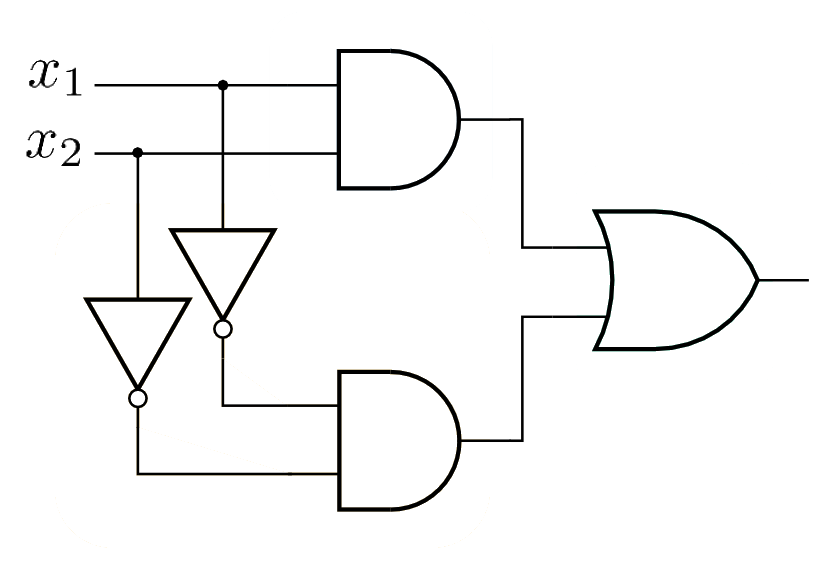
\includegraphics[width=0.41\textwidth]{circuits/6.3.9.png} % Replace 'path_to_image.png' with the actual path to your image file
			      		\end{figure}
			      	\end{center}
			      	
			      	\vspace{-60px}
			      	$$f(x_1, x_2)=x_1 x_2 + \bar{\,x_{1}}\bar{\, x_2}$$
			      	\vspace{-20px}
			      	\begin{table}[h!]
			      		\centering
			      		\begin{tabular}{cc|c}
			      			\hline
			      			$x_1$ & $x_2$ & $f(x_1, x_2)$ \\
			      			\hline
			      			0     & 0     & 1             \\
			      			0     & 1     & 0             \\
			      			1     & 0     & 0             \\
			      			1     & 1     & 1             \\
			      			\hline
			      		\end{tabular}
			      		\caption*{Corresponding logic table }
			      		\label{table:your_label}
			      	\end{table}
			      	        
			      	    
			      	\section{Analysis of a Logic Network}
			      	\text{Here we'll be looking at sequences of 0s and 1s sent by the input variables.} : 
			      	\begin{figure}[ht]
			      		\centering
			      		% Left Image
			      		\begin{minipage}{0.60\textwidth}
			      			\centering
			      			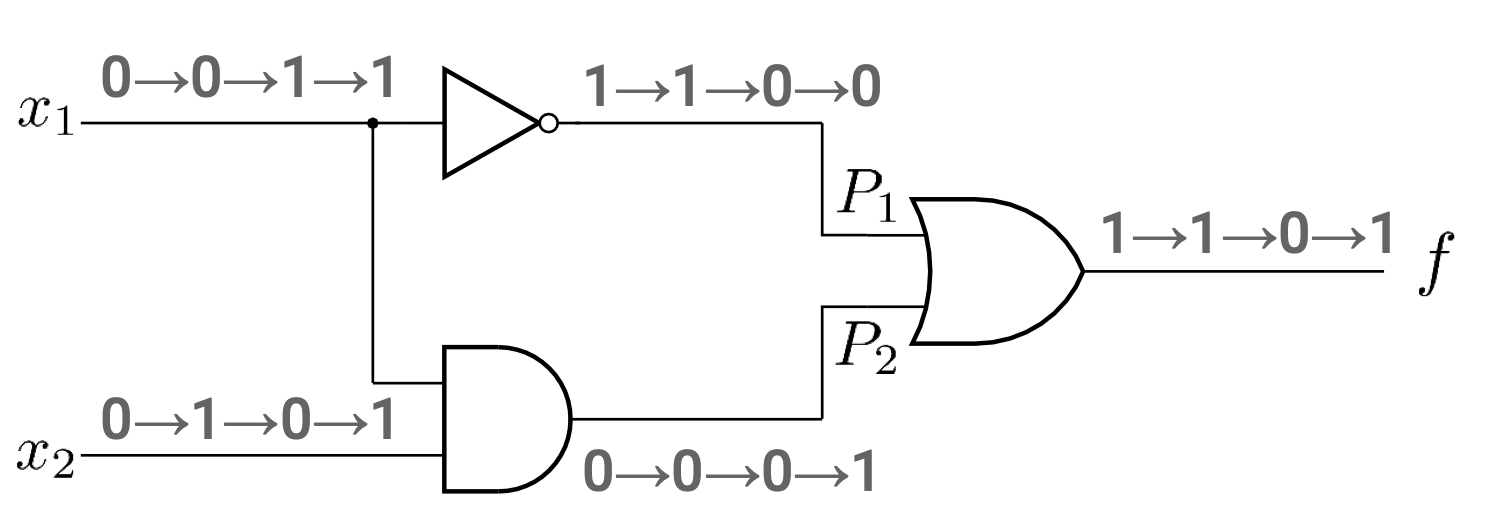
\includegraphics[width=\linewidth]{circuits/6.4.png}
			      			\caption*{$f(x_{1}, x_{2}) = \bar{\; x_1} + x_1 x_2 $}      \label{fig:left_image}
			      		\end{minipage}
			      		\hfill
			      		\begin{minipage}{0.37\textwidth}
			      			\centering
			      			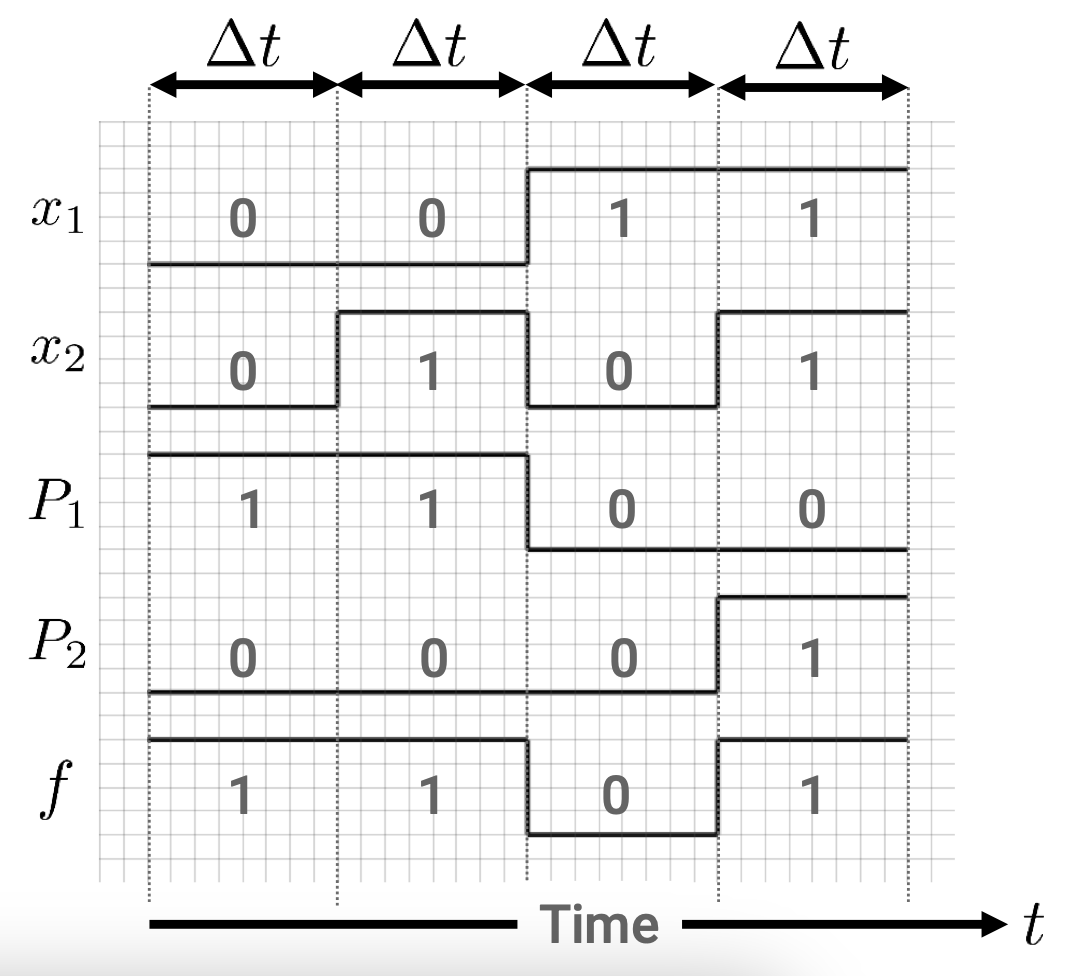
\includegraphics[width=\linewidth]{circuits/6.4_2.png} % 
			      			\caption*{\small Timing diagram representing the variations in electrical current magnitude over time}
			      			\label{fig:right_image}
			      		\end{minipage}
			      	\end{figure}
			      	
			      	\newpage
			      	\section*{Checking for Equivalence of Logic Networks}
			      	
			      	Two logic networks, represented by functions \( f \) and \( g \), are equivalent if:
			      	\begin{itemize}
			      		\item[] Their truth tables are identical, which is a verification through perfect induction.
			      		\item[] A sequence of algebraic manipulations using Boolean algebra can transform one logic expression into the other.
			      		\item[] Their Venn diagrams are the same, providing a simple visual aid for equivalence.
			      	\end{itemize}
			      	  
			      	\section*{Finding the Best Equivalent Network (Out of Scope)}
			      	  
			      	The best equivalent logic network is the simplest and cheapest in terms of the number of logic gates used. The process of finding the best equivalent expression is called \emph{minimization} and can be achieved through:
			      	\begin{itemize}
			      		\item[] A sequence of algebraic transformations, although it's not always clear which transformations to apply.
			      		\item[] Using the Karnaugh map, which is simpler than a truth table but becomes unmanageable by hand for more than 4 inputs.
			      		\item[] Automated techniques in synthesis tools (software) which can handle more complex networks efficiently.
			      	\end{itemize}
			      	  
			      	\section{The Venn Diagram}
			      	A Venn diagram is a visual representation of the relationships between sets. Each set is represented by a circle. The overlapping parts of circles represent common elements.
			      	
			      	\begin{figure}[htp] % This line sets the wrapfigure environment to place the figure on the right side and occupy half the text width
			      		\centering
			      		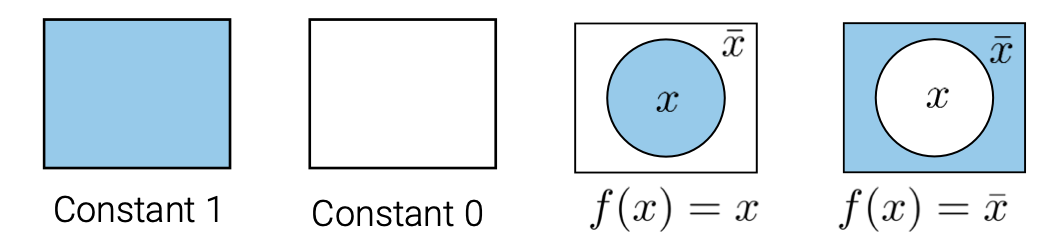
\includegraphics[width=0.60\textwidth]{circuits/6.5.png}
			      		
			      		\text{\small \; Basic Venn diagram representations}
			      	\end{figure}
			      	
			      	
			      	
			      	    
			      	\begin{center}
			      		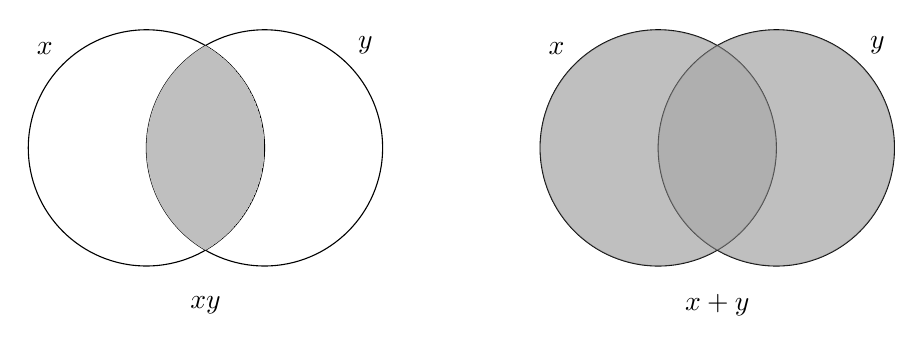
\begin{tikzpicture}
			      			% First drawing
			      			\node[circle, draw, minimum size=3cm, label=135:$x$] (A) at (0,0) {};
			      			\node[circle, draw, minimum size=3cm, label=45:$y$] (B) at (1.5,0) {};
			      			\begin{scope}
			      				\clip (0,0) circle (1.5cm);
			      				\clip (1.5,0) circle (1.5cm);
			      				\fill[gray!50] (A) circle (1.5cm);
			      			\end{scope}
			      			\node at (0.75,-2) {$xy$};
			      			  
			      			% Second drawing, shifted by 6.5cm to the right
			      			\begin{scope}[shift={(6.5,0)}] % Applying the calculated shift
			      				\begin{scope}[blend mode=screen]
			      					\node[circle, draw, minimum size=3cm, fill=gray, fill opacity=0.5, label=135:$x$] (A) at (0,0) {};
			      					\node[circle, draw, minimum size=3cm, fill=gray, fill opacity=0.5, label=45:$y$] (B) at (1.5,0) {};
			      				\end{scope}
			      				\node at (0.75,-2) {$x + y$};
			      			\end{scope}
			      		\end{tikzpicture}
			      	\end{center}
			      	
			      	\section{Network Equivalence Verification}
			      	  
			      	Venn Diagram Approach
			      	
			      	\[
			      		xy + \overline{x}z + yz \stackrel{?}{=} xy + \bar{x}z
			      	\]
			      	
			      	
			      	\noindent % Ensures no indentation for the entire group
			      	\begin{minipage}{.33\textwidth}
			      		\centering % Center the content inside the minipage
			      		\begin{venndiagram3sets}[labelA=\(x\), labelB=\(y\), labelC=\(z\)]
			      			\fillACapB
			      		\end{venndiagram3sets}
			      		xy % Replace with your desired caption or label
			      	\end{minipage}%
			      	\begin{minipage}{.33\textwidth}
			      		\centering
			      		\begin{venndiagram3sets}[labelA=\(x\), labelB=\(y\), labelC=\(z\)]
			      			\fillCNotA
			      		\end{venndiagram3sets}
			      		$\bar{x}z$
			      	\end{minipage}%
			      	\begin{minipage}{.33\textwidth}
			      		\centering
			      		\begin{venndiagram3sets}[labelA=\(x\), labelB=\(y\), labelC=\(z\)]
			      			\fillBCapC
			      		\end{venndiagram3sets}
			      		$yz$
			      	\end{minipage}
			      	
			      	\vspace{10px}
			      	Thus, the two expressions are equivalent. \newline \vspace*{20px}
			      	\noindent % Prevents indentation to align everything to the left.
			      	\begin{minipage}[c]{0.30\textwidth} % Adjust the width as needed for the first circuit
			      		\centering % Center the content
			      		\begin{venndiagram3sets}[labelA=\(x\), labelB=\(y\), labelC=\(z\)]
			      			\fillACapB
			      			\fillOnlyC
			      			\fillBCapC
			      		\end{venndiagram3sets}
			      		$ xy + \overline{x}z + yz $
			      	\end{minipage}%
			      	\hfill % Adds horizontal space between the minipages
			      	{\large $\equiv$} % Larger equivalence sign for better visibility
			      	\hfill % Adds horizontal space between the equivalence sign and the second circuit
			      	\begin{minipage}[c]{0.45\textwidth} % Adjust the width as needed for the second circuit
			      		\centering % Center the content
			      		\begin{venndiagram3sets}[labelA=\(x\), labelB=\(y\), labelC=\(z\)]
			      			\fillACapB
			      			\fillOnlyC
			      			\fillBCapC
			      		\end{venndiagram3sets}
			      		$ xy + \bar{x}z$
			      	\end{minipage}
			      	\hspace*{100px}
			      	
			      	\newpage
			      	
			      	
			      	\section{Boolean Algebra}
			      	      
			      	\subsection{Axioms}
			      	\begin{multicols}{2} % Start a two-column environment
			      		\begin{enumerate}
			      			\item[1a.] $0 \cdot 0 = 0$
			      			\item[1b.] $1 + 1 = 1$
			      			\item[2a.] $1 \cdot 1 = 1$
			      			\item[2b.] $0 + 0 = 0$
			      			\item[3a.] $0 \cdot 1 = 1 \cdot 0 = 0$
			      			\item[3b.] $1 + 0 = 0 + 1 = 1$
			      			\item[4a.] If $x = 0$, then $\bar{x} = 1$
			      			\item[4b.] If $x = 1$, then $\bar{x} = 0$
			      			\item[5a.] $x \cdot 0 = 0$
			      			\item[5b.] $x + 1 = 1$
			      			\item[6a.] $x \cdot 1 = x$
			      			\item[6b.] $x + 0 = x$
			      			\item[7a.] $x \cdot x = x$
			      			\item[7b.] $x + x = x$
			      			\item[8a.] $x \cdot \bar{x} = 0$
			      			\item[8b.] $x + \bar{x} = 1$
			      			\item[9.] $\bar{\bar{x}} = x$
			      			\item[10.] Commutative Property:
			      			      \begin{enumerate}
			      			      	\item Multiplication: \( x \cdot y = y \cdot x \)
			      			      	\item Addition: \( x + y = y + x \)
			      			      \end{enumerate}
                            \vspace*{60px} 
			      			\item[11.] Associative Property:
			      			      \begin{enumerate}
			      			      	\item Multiplication: \( x \cdot (y \cdot z) = (x \cdot y) \cdot z \)
			      			      	\item Addition: \( x + (y + z) = (x + y) + z \)
			      			      \end{enumerate}
			      			\item[12.] Distributive Property:
			      			      \begin{enumerate}
			      			      	\item Multiplication over Addition: \( x \cdot (y + z) = x \cdot y + x \cdot z \)
			      			      	\item $\quad x + y \cdot z = (x + y) \cdot (x + z)$
			      			      \end{enumerate}
			      			\item[13.] Absorption (covering):
			      			      \begin{enumerate}
			      			      	\item $x + x \cdot y = x$
			      			      	\item[b.] $x \cdot (x + y) = x$
			      			      \end{enumerate}
			      			\item[14.] Combining:
			      			      \begin{enumerate}
			      			      	\item $x \cdot y + x \cdot \bar{y} = x$
			      			      	\item $(x + y) \cdot (x + \bar{y}) = x$ 
			      			      \end{enumerate}
			      			      \vspace*{20px}
			      			\item[15.] DeMorgan's theorem:
			      			      \begin{enumerate}
			      			      	\item $\bar{x} \cdot \bar{y} = \overline{x + y}$
			      			      	\item $\bar{x} + \bar{y} = \overline{x \cdot y}$
			      			      \end{enumerate}
			      			\item[16.] Redundancy:
			      			      \begin{enumerate}
			      			      	\item $x + \bar{x} \cdot y = x + y$
			      			      	\item $x \cdot (\bar{x} + y) = x \cdot y$
			      			      \end{enumerate}
			      			\item[17.] Consensus:
			      			      \begin{enumerate}
			      			      	\item $x \cdot y + y \cdot z + \bar{x} \cdot z = x \cdot y + \bar{x} \cdot z$
			      			      	\item $(x + y) \cdot (y + z) \cdot (\bar{x} + z) = (x + y) \cdot (\bar{x} + z)$
			      			      \end{enumerate}
			      		\end{enumerate}
			      		        
			      	\end{multicols} % End the two-column environment
			      	            
			      	        
			      	        
			      	\chapter{Digital Logic (PART II)}
			      	\section{Logic Synthesis}
			      	\subsection{Minterms and Maxterms}
			      	\textit{Personal Remark. I changed the expression of the function for the product as it was clearer to my sens} \newline
			      	\vspace{10px}
			      	\textit{Personal Remark.2. This process ressembles a lot what we've seen in AICC I, with CNF and DNF.} \newline
			      	\vspace{10px}
			      	\textit{These two functions correspond to ways of representing binary numbers like we're used but using n-variable vectors. Here i is the number we're representing $m_i$ the corresponding "variable" minterm representation and $M_i$ maxterm's}\newline
			      	\vspace{10px}
			      	Let a product of n variables $f(x_{1}, x_{2}, \ldots, x_{n}) = \prod_{j=1}^{n}x_{j} = x_{1} \times x_{2} \ldots \times x_n = i = m_i$ in which each of the n variables only appear once, this is called a \textbf{minterm}. \newline
			      	\vspace{5px}
			      	Let a sum of n variables $f(x_{1}, x_{2}, \ldots, x_{n}) = \sum_{j=1}^{n}x_{j} = x_{1} + x_{2} + \ldots + x_n = i = M_i$ in which each of the n variables only appear once, this is called a \textbf{maxterm}. \newline
			      	
			      	\vspace*{-10px}
			      	\subsection{Examples}
			      	\subsubsection*{Minterms}
			      	\textit{To make it simple, $1 \rightarrow x, \; 0 \rightarrow \overline{x} $} \newline
			      	
			      	Let $ n = 3, i = 5$:\newline
			      	
			      	$ 5 = \underline{101}_2$
			      	thus $m_5 = x_1 \overline{x}_2 x_3$ \newline
			      	Let $n=5, i=3$:\newline
			      	$ 3 = \underline{00011}_2$
			      	thus $m_3 = \overline{x}_1 \overline{x}_2 x_3 \overline{x}_4 \overline{x}_5$ \newline
			      	
			      	\newpage
			      	\subsubsection{Maxterms}
			      	Maxterms are calculated as $M_i = \overline{m}_i$ \newline
			      	Let $ n = 3, i = 5$:
			      	\newline \textit{Using De Morgan's Law :}
			      	\begin{itemize}
			      		\item[]We have :
			      		      \begin{itemize}
			      		      	\item[] $m_5 = x_1 \overline{x}_2 x_3$
			      		      \end{itemize}
			      		\item[]thus :
			      		      \begin{itemize}
			      		      	\item[] $M_5 = \overline{m_5} =  \overline{x_1 \overline{x}_2 x_3} = \overline{x}_1 + x_2 + \overline{x}_3$ \newline
			      		      \end{itemize}
			      	\end{itemize}
			      	
			      	Let $n=5, i=3$:
			      	\begin{itemize}
			      		\item[]We have :
			      		      \begin{itemize}
			      		      	\item[] $m_3 = \overline{x}_1 \overline{x}_2 x_3 \overline{x}_4 \overline{x}_5$
			      		      \end{itemize}
			      		\item[]thus :
			      		      \begin{itemize}
			      		      	\item[] $M_3 = \overline{m_3} =  \overline{\overline{x}_1 \overline{x}_2 \overline{x_3} x_4 x_5} = x_1 + x_2 + x_3 + \overline{x}_4 + \overline{x}_5$ \newline
			      		      \end{itemize}
			      	\end{itemize}
			      	\begin{table}[h!]
			      		\centering
			      		\begin{tabular}{|c|c|c|c|>{\columncolor[HTML]{E0E0E0}}c|>{\columncolor[HTML]{B2DFDB}}c|}
			      			\hline
			      			\rowcolor[HTML]{FFFFFF} 
			      			\multicolumn{1}{|l|}{\cellcolor[HTML]{FFFFFF}Row number} & \(x_1\) & \(x_2\) & \(x_3\) & Minterm                                                & Maxterm                                                    \\ \hhline{|>{\arrayrulecolor[HTML]{FFFFFF}}->{\arrayrulecolor{black}}|-|-|-|-|-|}
			      			0                                                        & 0       & 0       & 0       & \(m_0 = \overline{x_1} \overline{x_2} \overline{x_3}\) & \(M_0 = x_1 + x_2 + x_3\)                                  \\ \hline
			      			1                                                        & 0       & 0       & 1       & \(m_1 = \overline{x_1} \overline{x_2} x_3\)            & \(M_1 = x_1 + x_2 + \overline{x_3}\)                       \\ \hline
			      			2                                                        & 0       & 1       & 0       & \(m_2 = \overline{x_1} x_2 \overline{x_3}\)            & \(M_2 = x_1 + \overline{x_2} + x_3\)                       \\ \hline
			      			3                                                        & 0       & 1       & 1       & \(m_3 = \overline{x_1} x_2 x_3\)                       & \(M_3 = x_1 + \overline{x_2} + \overline{x_3}\)            \\ \hline
			      			4                                                        & 1       & 0       & 0       & \(m_4 = x_1 \overline{x_2} \overline{x_3}\)            & \(M_4 = \overline{x_1} + x_2 + x_3\)                       \\ \hline
			      			5                                                        & 1       & 0       & 1       & \(m_5 = x_1 \overline{x_2} x_3\)                       & \(M_5 = \overline{x_1} + x_2 + \overline{x_3}\)            \\ \hline
			      			6                                                        & 1       & 1       & 0       & \(m_6 = x_1 x_2 \overline{x_3}\)                       & \(M_6 = \overline{x_1} + \overline{x_2} + x_3\)            \\ \hline
			      			7                                                        & 1       & 1       & 1       & \(m_7 = x_1 x_2 x_3\)                                  & \(M_7 = \overline{x_1} + \overline{x_2} + \overline{x_3}\) \\ \hline
			      		\end{tabular}
			      	\end{table}
			      	
			      	
			      	
			      	\newpage
			      	\subsection{Sum-of-Product (SOP) Form and Product-of-Sum (POS) Form}
			      	For a function f represented by a table, the rows where $f=1$ are represented by a sum of minterms, and the rows where $f=0$ are represented by a product of maxterms. \newline
			      	\textit{Remark} This is not the most optimal implementation of a function. \newline
			      	
			      	\subsubsection{Sum-of-Product (SOP) Form}
			      	\vspace*{10px}
			      	Consider a function \( f \) of \( n = 3 \) variables and the truth table below
			      	
			      	Canonical SOP form:
			      	\[
			      		f(x_1, x_2, x_3) = \sum (m_1, m_4, m_5, m_6) = \sum m(1, 4, 5, 6)
			      	\]
			      	
			      	\begin{center}
			      		\begin{tabular}{|c|c|c|c|}
			      			\hline
			      			\( x_1 \) & \( x_2 \) & \( x_3 \) & \( f \) \\
			      			\hline
			      			0         & 0         & 0         & 0       \\
			      			\hline
			      			\rowcolor{blue!25}
			      			0         & 0         & 1         & 1       \\
			      			\hline
			      			0         & 1         & 0         & 0       \\
			      			\hline
			      			0         & 1         & 1         & 0       \\
			      			\hline
			      			\rowcolor{blue!25}
			      			1         & 0         & 0         & 1       \\
			      			\hline
			      			\rowcolor{blue!25}
			      			1         & 0         & 1         & 1       \\
			      			\hline
			      			\rowcolor{blue!25}
			      			1         & 1         & 0         & 1       \\
			      			\hline
			      			1         & 1         & 1         & 0       \\
			      			\hline
			      		\end{tabular}
			      	\end{center}
			      	
			      	Thus the canonical SOP form :
			      	\begin{align*}
			      		  & f(x_1, x_2, x_3) = \overline{x_1} \overline{x_2} x_3 + x_1 \overline{x_2} \overline{x_3} + x_1 \overline{x_2} x_3 + x_1 x_2 \overline{x_3} \\
			      		  & = (\overline{x_1} + x_1) x_2 x_3 + \overline{x_1} (\overline{x_2} + x_2) x_3                                                               \\
			      		  & = 1 \cdot x_2 x_3 + \overline{x_1} \cdot 1 \cdot x_3                                                                                       \\
			      		  & = x_2 x_3 + \overline{x_1} x_3                                                                                                             
			      	\end{align*}
			      	
			      	
			      	\subsubsection{Product-of-Sum (POS) Form}
			      	Consider a function \( f \) of \( n = 3 \) variables and the truth table below
			      	\begin{center}
			      		\begin{tabular}{ccc|c}
			      			\( x_1 \) & \( x_2 \) & \( x_3 \) & \( f \) \\
			      			\hline
			      			0         & 0         & 0         & 0       \\
			      			0         & 0         & 1         & 1       \\
			      			0         & 1         & 0         & 0       \\
			      			0         & 1         & 1         & 0       \\
			      			1         & 0         & 0         & 1       \\
			      			1         & 0         & 1         & 1       \\
			      			1         & 1         & 0         & 1       \\
			      			1         & 1         & 1         & 0       \\
			      		\end{tabular}
			      	\end{center}
			      	\[
			      		f(x_1, x_2, x_3) = \prod (M_0, M_2, M_3, M_7)
			      	\]
			      	
			      	\[
			      		f(x_1, x_2, x_3) = M_0 \cdot M_2 \cdot M_3 \cdot M_7
			      	\]
			      	
			      	\[
			      		f(x_1, x_2, x_3) = (x_1 + x_2 + x_3)(x_1 + \overline{x_2} + x_3)(\overline{x_1} + x_2 + \overline{x_3})
			      	\]
			      	
			      	
			      	Complementing f :
			      	\[
			      		\overline{f}(x_1, x_2, x_3) = m_0 + m_2 + m_3 + m_7 = \overline{M_0} + \overline{M_2} + \overline{M_3} + \overline{M_7}
			      	\]
			      	
			      	\[
			      		\overline{f}(x_1, x_2, x_3) = \overline{M_0 \cdot M_2 \cdot M_3 \cdot M_7}
			      	\]
			      	
			      	By De Morgan's theorem
			      	
			      	\[
			      		f(x_1, x_2, x_3) = m_0 + m_2 + m_3 + m_7 = \overline{f}
			      	\]
			      	
			      	\textit{Personal Remark. Don't forget the objective here, these are just two ways, equivalent ways, to represent a function only using ORs and ANDs.}
			      	
			      	\section{NAND and NOR Logic Networks}
			      	
			      	
			      	\subsection{NAND GATE}
			      	\noindent % Prevents indentation to align everything to the left.
			      	\begin{minipage}[c]{0.30\textwidth} % Adjust the width as needed for the first circuit
			      		\centering % Center the content
			      		\begin{circuitikz} 
			      			\draw
			      			(0,0) node[nand port] (nand1) {}
			      			(nand1.in 1) node[anchor=east] {$x_1$}
			      			(nand1.in 2) node[anchor=east] {$x_2$}
			      			(nand1.out) node[anchor=west] {$\overline{x_1 \cdot x_2}$};
			      		\end{circuitikz}
			      	\end{minipage}%
			      	\hfill % Adds horizontal space between the minipages
			      	{\large $\equiv$} % Larger equivalence sign for better visibility
			      	\hfill % Adds horizontal space between the equivalence sign and the second circuit
			      	\begin{minipage}[c]{0.35\textwidth} % Adjust the width as needed for the second circuit
			      		\centering % Center the content
			      		\begin{minipage}[c]{1\textwidth} % Adjust the width as needed for the second circuit
			      			\centering
			      			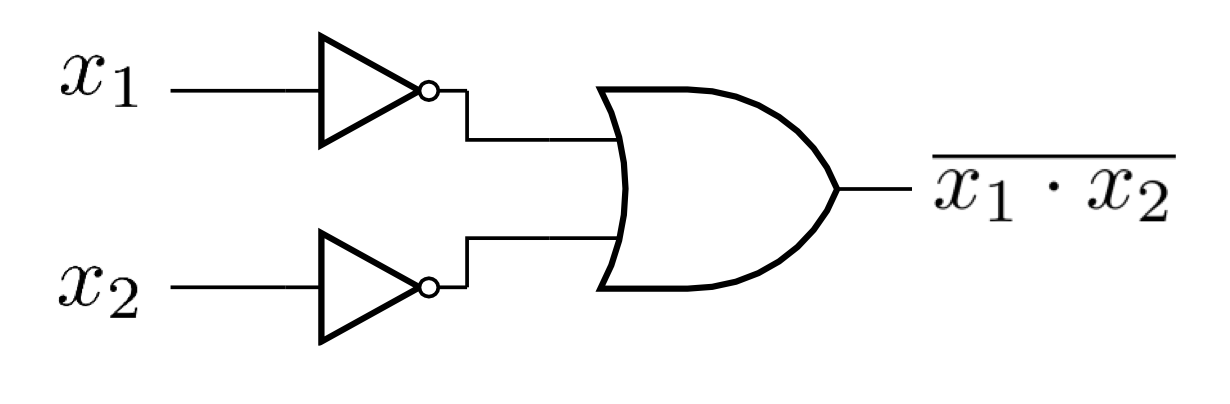
\includegraphics[width=1\textwidth]{circuits/6.9.1.png} % Replace 'path_to_image.png' with the actual path to your image file
			      		\end{minipage}
			      	\end{minipage}
			      	\hspace*{100px}
			      	
			      	$$f(x_1, x_2) = \overline{x_1 \cdot x_2} = \overline{x_1} + \overline{x_2}$$
			      	
			      	
			      	\subsubsection*{Logic Network with NAND Gates}
			      	
			      	Implement the following function in the SOP form with NAND gates:
			      	\begin{equation}
			      		f = x_2 + \overline{x_1 x_3}
			      	\end{equation}
			      	
			      	Algorithm: start by applying double inversion and, then, De Morgan's theorem to simplify the expression:
			      	\begin{align}
			      		f & = x_2 + \overline{x_1 x_3}                                      \\
			      		  & = \overline{\overline{x_2 + x_1 \overline{x_3}}}                \\
			      		  & = \overline{\overline{x_2} \cdot \overline{x_1 \overline{x_3}}} 
			      	\end{align}
			      	
			      	\subsection{NOR GATE}
			      	\noindent % Prevents indentation to align everything to the left.
			      	\begin{minipage}[c]{0.30\textwidth} % Adjust the width as needed for the first circuit
			      		\centering % Center the content
			      		\begin{circuitikz}
			      			\draw
			      			(0,0) node[nor port] (nor1) {}
			      			(nor1.in 1) node[anchor=east] {$x_1$}
			      			(nor1.in 2) node[anchor=east] {$x_2$}
			      			(nor1.out) node[anchor=west] {$\overline{x_1 + x_2}$};
			      		\end{circuitikz}
			      	\end{minipage}%
			      	\hfill % Adds horizontal space between the minipages
			      	{\large $\equiv$} % Larger equivalence sign for better visibility
			      	\hfill % Adds horizontal space between the equivalence sign and the second circuit
			      	\begin{minipage}[c]{0.6\textwidth} % Adjust the width as needed for the second circuit
			      		\centering
			      		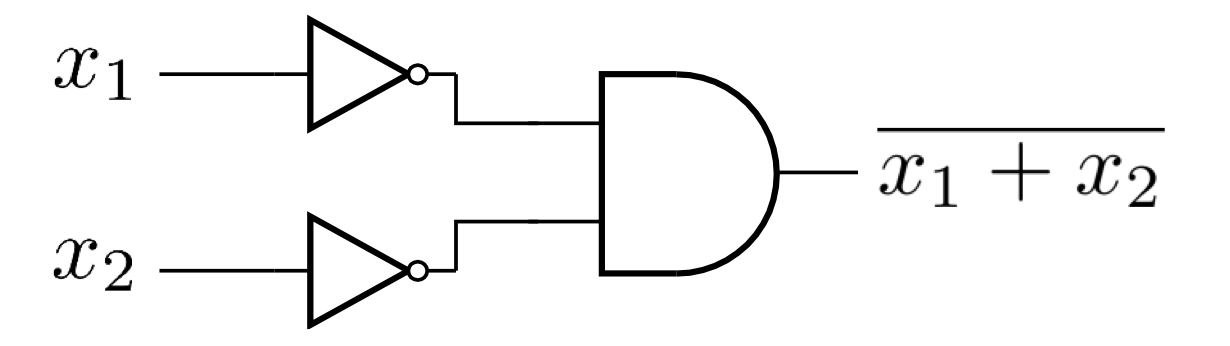
\includegraphics[width=0.6\textwidth]{circuits/6.9.2.png} % Replace 'path_to_image.png' with the actual path to your image file
			      	\end{minipage}
			      	\hspace*{100px}
			      	
			      	$$f(x_1, x_2) = \overline{x_1 + x_2} = \overline{x_1} \cdot \overline{x_2}$$
			      	
			      	        
			      	
			      	\subsubsection*{Logic Network with NOR Gates}
			      	Implement the following function in the POS form with NOR gates:
			      	\begin{equation}
			      		f = (x_1 + x_2)(x_2 + x_3)
			      	\end{equation}
			      	
			      	Algorithm: start by applying double inversion and, then, De Morgan's theorem to simplify the expression:
			      	\begin{align}
			      		f & = (x_1 + x_2)(x_2 + \overline{x_3})                                     \\
			      		  & = \overline{\overline{(x_1 + x_2)(x_2 + \overline{x_3})}}               \\
			      		  & = \overline{\overline{(x_1 + x_2)} + \overline{(x_2 + \overline{x_3})}} 
			      	\end{align}
			      	\section{incompletely Defined Functions}
			      	\subsection{Don't Care Condition}
			      	Don't care conditions occur in logic design when certain input combinations never occur, or their corresponding outputs do not affect the system behavior. 
			      	
			      	\subsection{Example}
			      	Consider \( x_1 \) and \( x_2 \) as inputs controlling two doors to a lion's cage. Here, \( x_1 \) is the control for the outer door and \( x_2 \) for the inner door. The truth table is as follows:
			      	
			      	\begin{center}
			      		\begin{tabular}{cc|c|l}
			      			\( x_1 \) & \( x_2 \) & \( f \) & Behavior                 \\
			      			\hline
			      			0         & 0         & 0       & Doors closed             \\
			      			0         & 1         & 1       & Outer closed, inner open \\
			      			1         & 0         & 1       & Outer open, inner closed \\
			      			1         & 1         & X       & Doors open (don't care)  \\
			      		\end{tabular}
			      	\end{center}
			      	
			      	The condition where both doors are open is a 'don't care' because it should never happen for safety reasons.
			      	
			      	\subsection{Incomplete Functions}
			      	A logic function with 'don't care' conditions is termed 'incompletely defined'. These conditions can be exploited to optimize the circuit by choosing don't care outputs to simplify the logic expression.
			      	
			      	\subsection{Sum of Products (SOP) Example}
			      	For the lion's cage control, with 'don't cares' the function can be expressed as:
			      	\[ f = \sum m(1,2) + D(3) \]
			      	
			      	\begin{itemize}
			      		\item Assuming \( D(3) = 0 \), the function simplifies to:
			      		      \[ f = \overline{x_1} x_2 + x_1 \overline{x_2} \]
			      		      using 5 gates and 8 inputs.
			      		\item Assuming \( D(3) = 1 \), the function simplifies further to:
			      		      \[ f = x_1 \bar{x}_2 + x_1 = x_1 + x_2 \]
			      		      using an OR gate and redundancy rules.
			      	\end{itemize}
			      	
			      	\textit{Adding don't care values sometimes allows for a simpler implementation.}
			      	\section{Even and Odd Detectors (XNOR and XOR Gates)}
			      	\subsection{XOR Gate}
			      	\textit{True when one and only one input is True}
			      	The exclusif OR (XOR) gate is represented with the table below :
			      	\begin{table}[h]
			      		\centering
			      		\begin{tabular}{|c|c|c|}
			      			\hline
			      			\( x_1 \) & \( x_2 \) & \( f \) \\
			      			\hline
			      			0         & 0         & 0       \\
			      			0         & 1         & 1       \\
			      			1         & 0         & 1       \\
			      			1         & 1         & 0       \\
			      			\hline
			      		\end{tabular}
			      	\end{table}
			      	
			      	and looks like:
			      	\vspace*{-10px}
			      	\begin{center}
			      		\begin{minipage}[c]{0.45\textwidth} % Adjust the width as needed for the second circuit
			      			\centering
			      			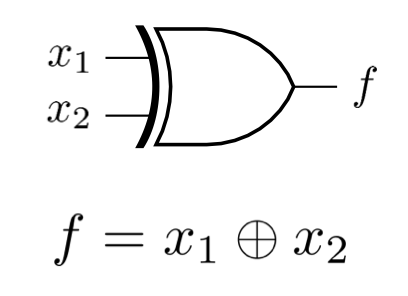
\includegraphics[width=0.45\textwidth]{circuits/6.11.1.png} % Replace 'path_to_image.png' with the actual path to your image file
			      		\end{minipage}
			      	\end{center}
			      	
			      	\subsection{XNOR Gate}
			      	The exclusif NOR (XNOR) gate is represented with the table below :
			      	\textit{True when both inputs are the same.}
			      	\vspace*{-10px}
			      	\begin{table}[h]
			      		\centering
			      		\begin{tabular}{|c|c|c|}
			      			\hline
			      			\( x_1 \) & \( x_2 \) & \( f \) \\
			      			\hline
			      			    
			      			0         & 0         & 1       \\
			      			0         & 1         & 0       \\
			      			1         & 0         & 0       \\
			      			1         & 1         & 1       \\
			      			\hline
			      		\end{tabular}
			      	\end{table}
			      	
			      	and looks like:
			      	\begin{center}
			      		\begin{minipage}[c]{0.45\textwidth} % Adjust the width as needed for the second circuit
			      			\centering
			      			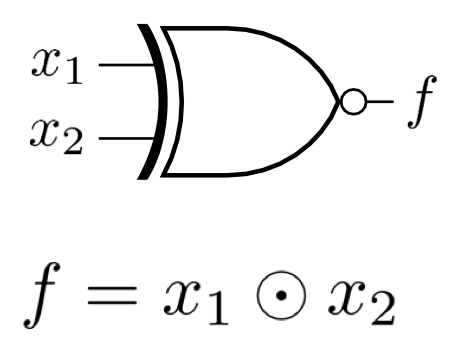
\includegraphics[width=0.45\textwidth]{circuits/6.11.2.png} % Replace 'path_to_image.png' with the actual path to your image file
			      		\end{minipage}
			      	\end{center}
			      	
			      	\section{Design Example}
			      	\subsection{Number Display}
			      	Here we will be designing a logic circuit to drive a seven-segment display .
			      	\begin{center}
			      		\begin{minipage}[c]{0.80\textwidth} % Adjust the width as needed for the second circuit
			      			\centering
			      			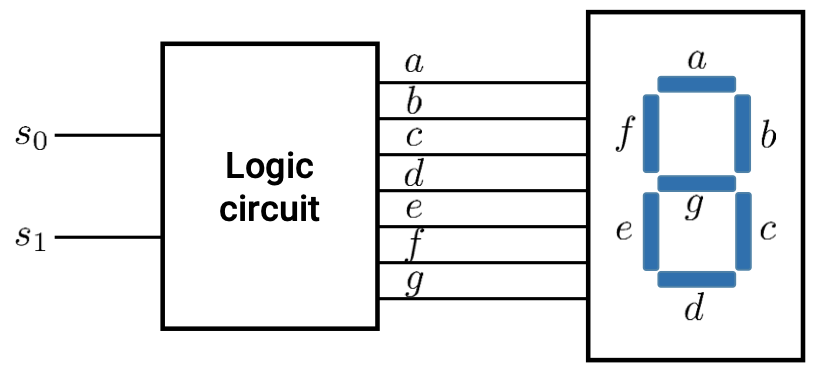
\includegraphics[width=0.80\textwidth]{circuits/6.12.1.png} 
			      		\end{minipage}
			      	\end{center}
			      	We can derive one logic function per output of the table below:
			      	\begin{table}[h!]
			      		\centering
			      		\begin{tabular}{|c|c|c|c|c|c|c|c|c|}
			      			\hline
			      			\multicolumn{2}{|c|}{} & \multicolumn{7}{c|}{Output} \\
			      			\hhline{|~|-|-------|}
			      			\( S_1 \) & \( S_0 \) & a & b & c & d & e & f & g \\
			      			\hline
			      			0         & 0         & 1 & 1 & 1 & 1 & 1 & 1 & 0 \\
			      			\hline
			      			0         & 1         & 0 & 1 & 1 & 0 & 0 & 0 & 0 \\
			      			\hline
			      			1         & 0         & 1 & 1 & 0 & 1 & 1 & 0 & 1 \\
			      			\hline
			      			1         & 1         & 1 & 1 & 1 & 1 & 0 & 0 & 1 \\
			      			\hline
			      		\end{tabular}
			      	\end{table}
			      	\vspace{-10px}
			      	\begin{align*}
			      		a(s_0, s_1) & = M_1 = s_1 + \overline{s_0}                                               \\
			      		b(s_0, s_1) & = 1                                                                        \\
			      		c(s_0, s_1) & = M_2 = s_1 + s_0                                                          \\
			      		d(s_0, s_1) & = M_1 = s_1 + \overline{s_0} = a(s_0, s_1)                                 \\
			      		e(s_0, s_1) & = M_1 \cdot M_3 = m_0 + m_2 = s_1 \overline{s_0} + s_1s_0 = \overline{s_0} \\
			      		f(s_0, s_1) & = m_0 = \overline{s_1 s_0}                                                 \\
			      		g(s_0, s_1) & = M_0 \cdot M_1 = m_2 + m_3 = s_1 \overline{s_0} + s_1s_0 = s_1            
			      	\end{align*}
			      	
			      	\newpage
			      	\subsection{Multiplexer}
			      	A \textit{multiplexer}, or MUX, is a circuit that selects one of several inputs to pass to the output based on the value of one or more select inputs.\newline
			      	\noindent % Prevents indentation to align everything to the left.
			      	\begin{minipage}[c]{0.45\textwidth} % Adjust the width as needed for the first circuit
			      		\centering % Center the content
			      		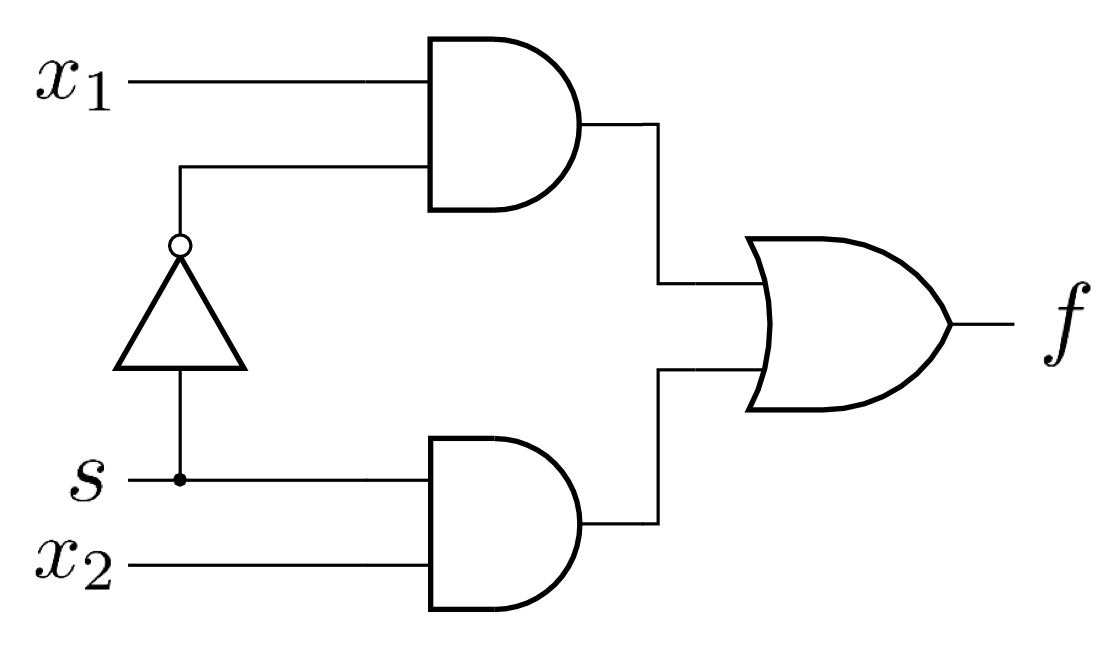
\includegraphics[width=0.9\linewidth]{circuits/6.12.2.png} % Adjust the image width as needed
			      	\end{minipage}%
			      	\hfill % Adds horizontal space between the minipages
			      	{\large $\equiv$} % Larger equivalence sign for better visibility
			      	\hfill % Adds horizontal space between the equivalence sign and the second circuit
			      	\begin{minipage}[c]{0.50\textwidth} % Adjust the width as needed for the second circuit
			      		\centering
			      		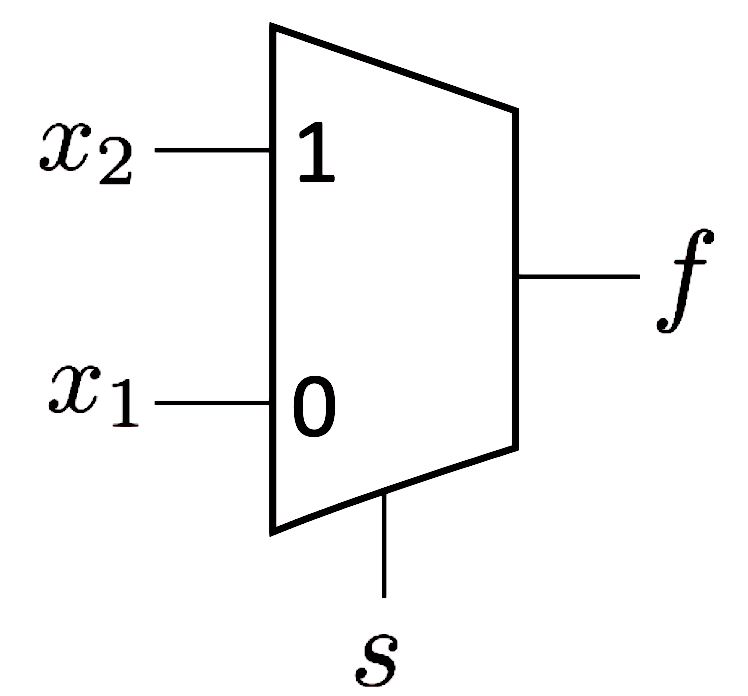
\includegraphics[width=0.6\linewidth]{circuits/6.12.2_2.png} % Adjust the image width as needed
			      	\end{minipage}
			      	Reading the truth table, we can derive the following logic functions:
			      	\begin{table}[h!]
			      		\centering
			      		\begin{tabular}{cccc}
			      			\hline
			      			$s$ & $x_1$ & $x_2$ & $f$ \\
			      			\hline
			      			0   & 0     & 0     & 0   \\
			      			0   & 0     & 1     & 0   \\
			      			0   & 1     & 0     & 1   \\
			      			0   & 1     & 1     & 1   \\
			      			1   & 0     & 0     & 0   \\
			      			1   & 0     & 1     & 1   \\
			      			1   & 1     & 0     & 0   \\
			      			1   & 1     & 1     & 1   \\
			      			\hline
			      		\end{tabular}
			      	\end{table}
			      	\[
			      		f(s, x_1, x_2) = \overline{s} x_1 x_2 + \overline{s} x_1 \overline{x_2} + s \overline{x_1} x_2 + s x_1 x_2
			      	\]
			      	
			      	\[
			      		f(s, x_1, x_2) = \overline{s}x_1 (\overline{x_2} + x_2) + s(\overline{x_1} + x_1)x_2
			      	\]
			      	
			      	\[
			      		= \overline{s}x_1 + sx_2
			      	\]
			      	
			      	
			      	
			      	If there are \( n \) inputs to select from, the number of select signals required in a MUX can be determined by:
			      	
			      	\[
			      		\text{Number of select signals} = \left\lceil \log_2 n \right\rceil
			      	\]
			      	
			      	\textit{Examples:}
			      	\begin{itemize}
			      		\item[] Two inputs: one select signal to choose between inputs indexed as `0' and `1'
			      		\item[] Four inputs: two select signals (indices 0, 1, 2, 3)
			      		\item[] Eight inputs: three select signals (indices 0, 1, 2, \ldots, 7)
			      	\end{itemize}
			      	
			      	
			      	
			      	\chapter{Digital Logic (PART III)}
			      	\section{Adders}
			      	\subsection{Addition of two 1-bit binary numbers}
			      	In this section, we will be adding two 1-bit binary numbers. The truth table is as follows:
			      	\begin{itemize}
			      		\item[] The resulting sum is at most on two bits:
			      		      \begin{itemize}
			      		      	\item[-] the rightmost bit is called \textit{sum} (s)
			      		      	\item[-] the leftmost bit is called \textit{carry} (c); it is produced as a carry-out when both bits being added are logical one
			      		      \end{itemize}
			      	\end{itemize}
			      	
			      	
			      	\[
			      		\begin{array}{cccccc}
			      			            & $x$       \\
			      			+           & $y$       \\
			      			\hline
			      			$c (carry)$ & $s (sum)$ \\
			      		\end{array}
			      	\]
			      	    
			      	\subsection{Binary Addition Examples}
			      	
			      	\[
			      		\begin{array}{cccccc}
			      			  & 0 \\
			      			+ & 0 \\
			      			\hline
			      			0 & 0 \\
			      		\end{array}
			      	\]
			      	\[
			      		\begin{array}{cccccc}
			      			  & 0 \\
			      			+ & 1 \\
			      			\hline
			      			0 & 1 \\
			      		\end{array}
			      	\]
			      	\[
			      		\begin{array}{cccccc}
			      			  & 1 \\
			      			+ & 0 \\
			      			\hline
			      			0 & 1 \\
			      		\end{array}
			      	\]
			      	\[
			      		\begin{array}{cccccc}
			      			  & 1 \\
			      			+ & 1 \\
			      			\hline
			      			1 & 0 \\
			      		\end{array}
			      	\]
			      	
			      	\newpage
			      	\subsection{Half-Adder}
			      	\textit{Personal Remark. The circuits shown in this part might seem a bit overwhelming, I suggest you first try to understand what the full and half adders are, then try to understand the corresponding circuits.} 
			      	\newline
			      	\vspace{10px}
			      	A half adder is a digital circuit that adds two single-bit binary numbers and outputs a sum and a carry. 
			      	
			      	
			      	\begin{table}[h!]
			      		\centering
			      		\begin{tabular}{cccc}
			      			\hline
			      			$x$ & $y$ & $s$ & $c$ \\
			      			\hline
			      			0   & 0   & 0   & 0   \\
			      			0   & 1   & 1   & 0   \\
			      			1   & 0   & 1   & 0   \\
			      			1   & 1   & 0   & 1   \\
			      			\hline
			      		\end{tabular}
			      	\end{table}
			      	
			      	Using SOP form, we can derive the following logic functions:
			      	$$ s = \overline{x}y + x\overline{y} = x \xor y$$
			      	$$ c = xy$$
			      	
			      	Thus the Digital Logic Circuit : 
			      	\begin{center}
			      		\begin{minipage}[c]{0.60\textwidth} % Adjust the width as needed for the second circuit
			      			\centering
			      			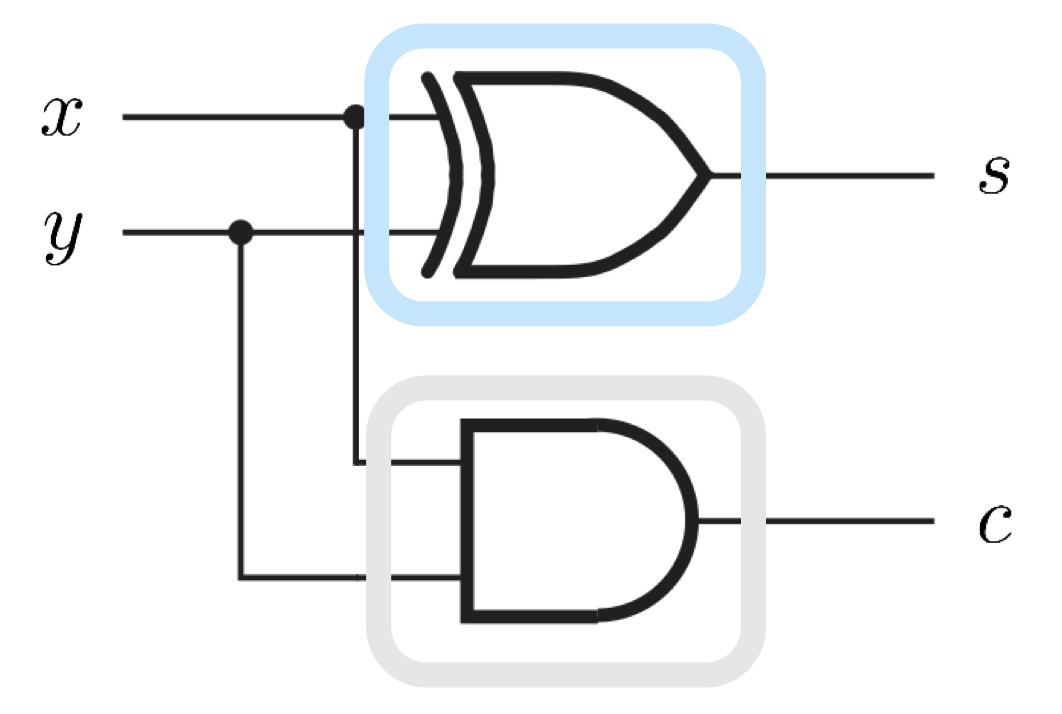
\includegraphics[width=0.60\textwidth]{circuits/7.1.3.png} % Replace 'path_to_image.png' with the actual path to your image file
			      		\end{minipage}
			      		
			      	\end{center}
			      	Also represented as :
			      	\begin{center}
			      		\begin{minipage}[c]{0.60\textwidth} % Adjust the width as needed for the second circuit
			      			\centering
			      			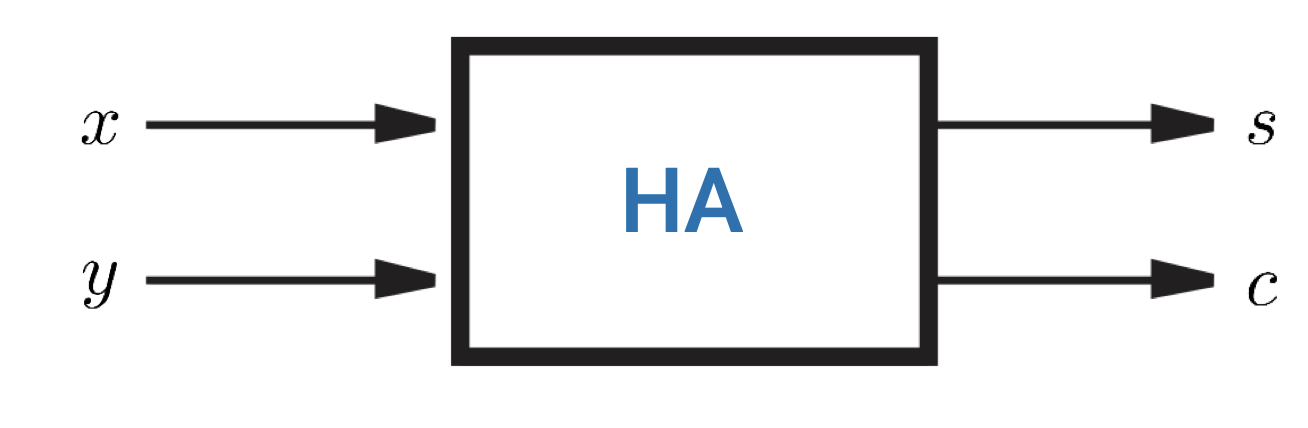
\includegraphics[width=0.60\textwidth]{circuits/7.1.3_2.png} % Replace 'path_to_image.png' with the actual path to your image file
			      		\end{minipage}
			      		
			      	\end{center}
			      	\newpage
			      	
			      	\subsection{Addition of Two N-Bit Binary Numbers}
			      	A binary \textit{n}-bit adder computes the sum of two \textit{n}-bit numbers $x$ and $y$ within the range of $0 \leq x, y \leq 2^n - 1$, with a carry-in $c_{\text{in}} \in \{0, 1\}$. It produces:
			      	
			      	\begin{itemize}
			      		\item[] A sum $s$, where $0 \leq s \leq 2^n - 1$.
			      		\item[] A carry-out $c_{\text{out}} \in \{0, 1\}$, satisfying the equation:
			      	\end{itemize}
			      	
			      	\begin{equation}
			      		x + y + c_{\text{in}} = 2^n c_{\text{out}} + s
			      	\end{equation}
			      	
			      	The solution to the equation is given by:
			      	
			      	\begin{equation}
			      		s = (x + y + c_{\text{in}}) \mod 2^n
			      	\end{equation}
			      	
			      	\begin{equation}
			      		c_{\text{out}} = 
			      		\begin{cases} 
			      			1 & \text{if } (x + y + c_{\text{in}}) \geq 2^n (overflow) \\
			      			0 & \text{otherwise}                                       
			      		\end{cases}
			      		= \left\lfloor \frac{(x + y + c_{\text{in}})}{2^n} \right\rfloor
			      	\end{equation}
			      	\subsection{Addition of Two N-Bit Binary Numbers}
			      	
			      	\begin{itemize}
			      		\item[] It is impractical to start from the truth tables for \( n \)-bit addition.
			      		\item[] Iterative approach:
			      		      \begin{itemize}
			      		      	\item[] Add each pair of bits at the position \( i \), where \( 0 \leq i < n \).
			      		      	\item[] The addition at the bit position \( i \) needs to include a carry-in at the position \( i \) (corresponding to the carry-out at the position \( i - 1 \)).
			      		      \end{itemize}
			      		\item[] The 1-bit adder reduces to a primitive module (new block that summarizes the circuit) called \textit{full-adder (FA)} with three binary inputs and two binary outputs such that \newline \( x_i + y_i + c_i = 2c_{i+1} + s_i \).
			      	\end{itemize}
			      	\newpage
			      	\subsection{Full-Adder}
			      	A full adder, on the other hand, is a digital circuit that adds three single-bit binary numbers: the two bits to be added plus an additional carry-in bit. This carry-in bit is the carry from the addition of two lower significant bits. The full adder outputs a sum and a carry-out.
			      	
			      	\begin{itemize}
			      		\item[] Truth table:
			      		      \begin{center}
			      		      	\begin{tabular}{cccc|cc}
			      		      		\( x_i \) & \( y_i \) & \( c_i \) &   & \( s_i \) & \( c_{i+1} \) \\
			      		      		\hline
			      		      		0         & 0         & 0         &   & 0         & 0             \\
			      		      		0         & 0         & 1         &   & 1         & 0             \\
			      		      		0         & 1         & 0         &   & 1         & 0             \\
			      		      		0         & 1         & 1         &   & 0         & 1             \\
			      		      		1         & 0         & 0         &   & 1         & 0             \\
			      		      		1         & 0         & 1         &   & 0         & 1             \\
			      		      		1         & 1         & 0         &   & 0         & 1             \\
			      		      		1         & 1         & 1         &   & 1         & 1             \\
			      		      	\end{tabular}
			      		      \end{center}
			      		\item[] Logical expressions:
			      		      \begin{align*}
			      		      	s_i     & = \bar{x_i}\bar{y_i} c_i + \bar{x}_i y_i \bar{c}_i + x_i \bar{y}_i \bar{c}_i + x_i y_i c_i \\
			      		      	        & = (x_i y_i + \bar{x}_i \bar{y}_i)c_i + (\bar{x}_i y_i + x_i \bar{y}_i)\bar{c}_i            \\
			      		      	        & = \overline{(x_i \xor y_i)}c_i + (x_i \xor y_i)\bar{c}_i = x_i \xor y_i \xor c_i           \\
			      		      	\\
			      		      	c_{i+1} & = \bar{x}_i y_i c_i + x_i \bar{y}_i c_i + x_i y_i \bar{c}_i + x_i y_i c_i                  \\
			      		      	        & = (\bar{x}_i y_i + x_i \bar{y}_i)c_i + x_i y_i(\bar{c}_i + c_i)                            \\
			      		      	        & = (x_i \xor y_i)c_i + x_i y_i                                                              \\
			      		      	        & = x_i y_i + x_i c_i + y_i c_i                                                              \\
			      		      \end{align*}
			      		      
			      		       
			      	\end{itemize}
			      	
			      	\begin{itemize}
			      		\item[] Thus:
			      		      \begin{align*}
			      		      	s_i     & = x_i \xor y_i \xor c_i                                     \\
			      		      	c_{i+1} & = (x_i \xor y_i)c_i + x_i y_i = x_i y_i + x_i c_i + y_i c_i 
			      		      \end{align*}
			      		\item[] With Logic Circuit:
			      		      
			      		      
			      		      \begin{center}
			      		      	\begin{minipage}[c]{0.60\textwidth} % Adjust the width as needed for the second circuit
			      		      		\centering
			      		      		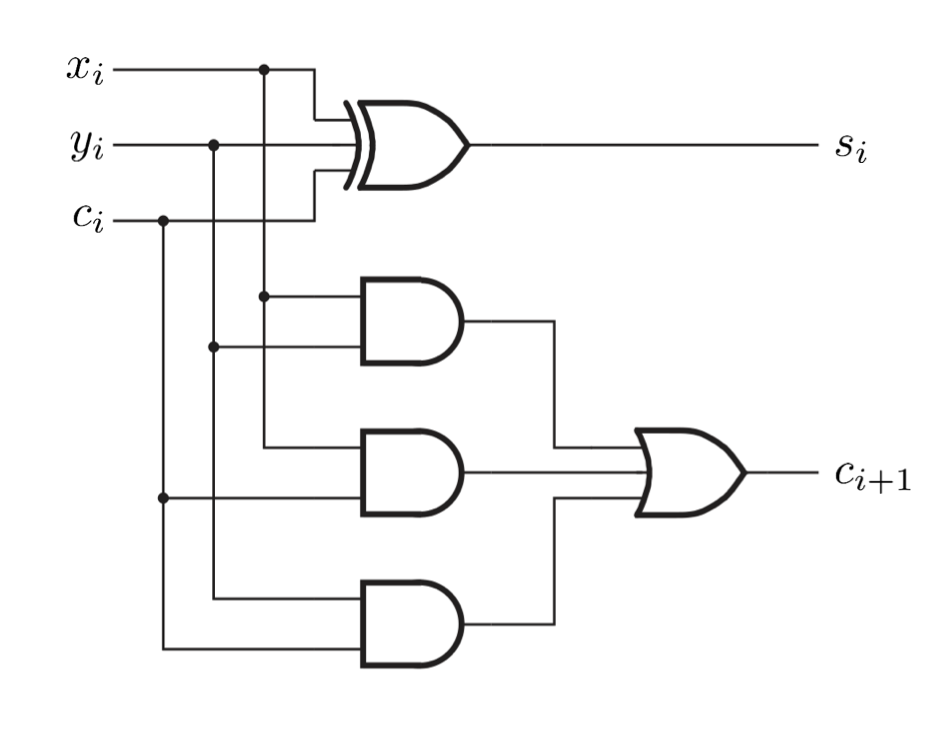
\includegraphics[width=0.60\textwidth]{circuits/8.1.6.png} % Replace 'path_to_image.png' with the actual path to your image file
			      		      	\end{minipage}
			      		      	  
			      		      \end{center}
			      		      
			      		      \vspace{10px}
			      		\item[] Also represented as :
			      		      \begin{center}
			      		      	\begin{minipage}[c]{0.60\textwidth} % Adjust the width as needed for the second circuit
			      		      		\centering
			      		      		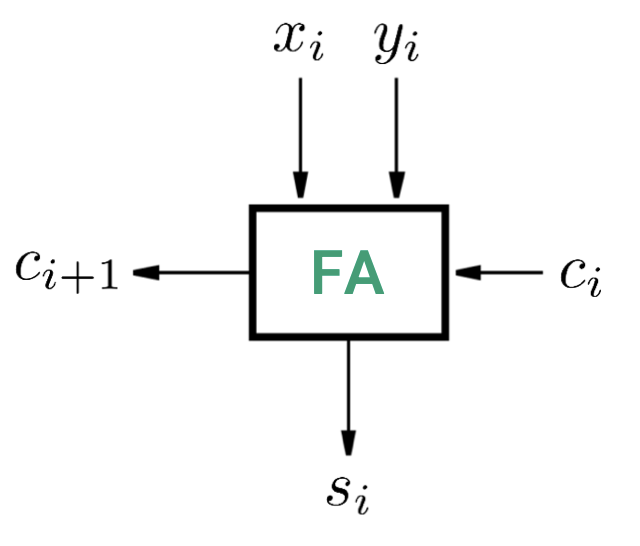
\includegraphics[width=0.60\textwidth]{circuits/8.1.6_2.png} % Replace 'path_to_image.png' with the actual path to your image file
			      		      	\end{minipage}
			      		      	
			      		      \end{center}
			      	\end{itemize}
			      	
			      	
			      	\subsection{Basic Ripple-Carry Adder}
			      	Is a chain of full adders that add two \( n \)-bit binary numbers. It's called a \textbf{ripple-carry} adder because the carry-out of each full adder ripples (goes through the full adder chain) into the carry-in of the next full adder.
			      	
			      	\vspace{10px}
			      	
			      	It looks like this:
			      	\begin{center}
			      		\begin{minipage}[c]{0.80\textwidth} % Adjust the width as needed for the second circuit
			      			\centering
			      			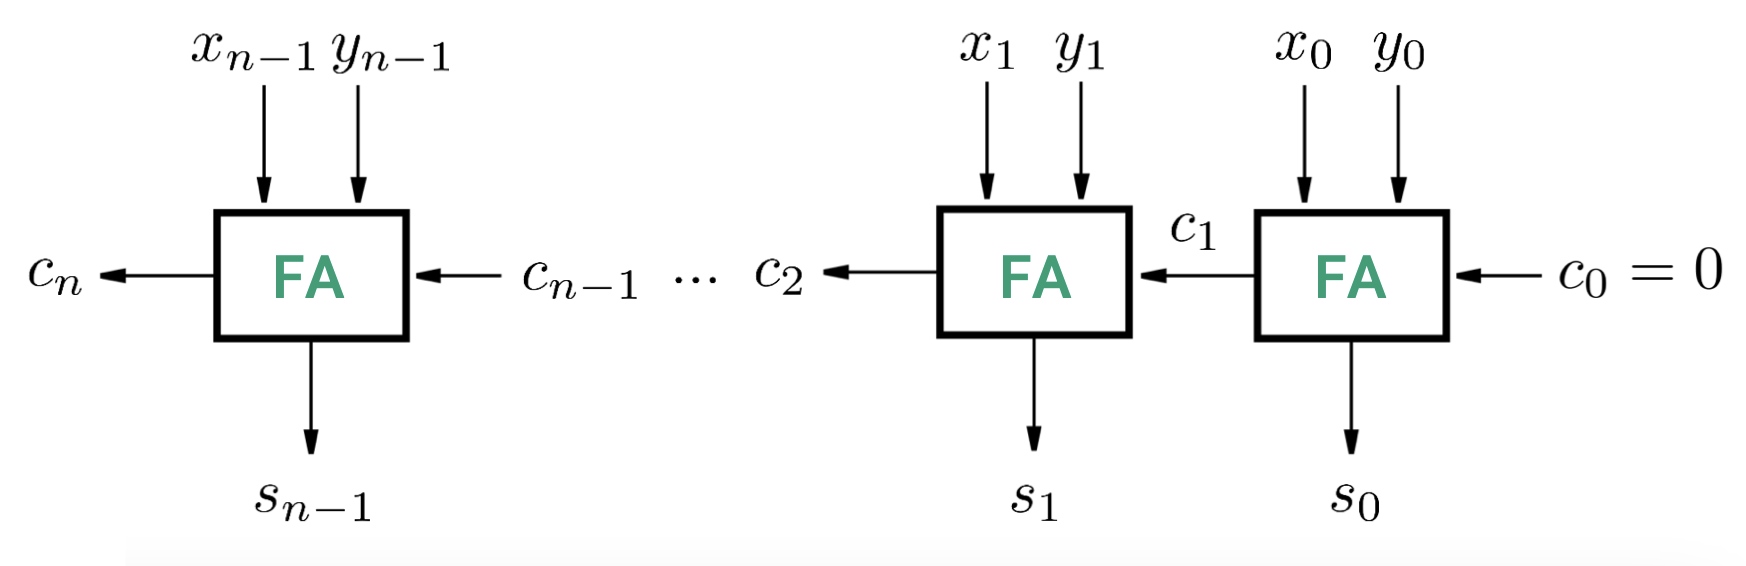
\includegraphics[width=0.80\textwidth]{circuits/8.1.7.png} % Replace 'path_to_image.png' with the actual path to your image file
			      		\end{minipage}
			      		  
			      	\end{center}
			      	
			      	
			      	\section{Subtractors}
			      	\textit{Same but with substraction and borrows.}
			      	\subsection{Subtraction of Two 1-Bit Binary Numbers}
			      	In this section, we will be subtracting two 1-bit binary numbers. The truth table is as follows:
			      	\begin{itemize}
			      		\item[] The resulting difference is at most on two bits:
			      		      \begin{itemize}
			      		      	\item[-] the rightmost bit is called \textit{difference} (d)
			      		      	\item[-] the leftmost bit is called \textit{borrow} (b); it is produced as a borrow-out when the subtrahend is greater than the minuend
			      		      \end{itemize}
			      	\end{itemize}
			      	
			      	Let $b$ be the borrow-in, $x$ be the minuend, and $y$ be the subtrahend and d the difference. 
			      	\[
			      		\begin{array}{cccccc}
			      			&$b$ \\
			      			  &   & $x$ \\
			      			- &   & $y$ \\
			      			\hline
			      			  &   & $d$ \\
			      		\end{array}
			      	\]
			      	
			      	\subsection{Binary Subtraction Examples}
			      	
			      	
			      	
			      	\[
			      		\begin{array}{cccc}
			      			&0 & \\
			      			  &   & 0 &   \\
			      			- &   & 0 &   \\
			      			\hline
			      			  &   & 0 &   \\
			      		\end{array}
			      	\]
			      	\[
			      		\begin{array}{cccc}
			      			&1 & \\
			      			  &   & 0 &   \\
			      			- &   & 1 &   \\
			      			\hline
			      			  &   & 1 &   \\
			      		\end{array}
			      	\]
			      	\[
			      		\begin{array}{cccc}
			      			& 0 & \\
			      			  &   & 1 &   \\
			      			- &   & 0 &   \\
			      			\hline
			      			  &   & 1 &   \\
			      		\end{array}
			      	\]
			      	\[
			      		\begin{array}{cccc}
			      			& 0 & \\
			      			  &   & 1 &   \\
			      			- &   & 1 &   \\
			      			\hline
			      			  &   & 0 &   \\
			      		\end{array}
			      	\]
			      	
			      	\subsection{Subtraction of Two N-Bit Unsigned Numbers}
			      	
			      	\begin{itemize}
			      		\item[] It is impractical to start from the truth tables for \( n \)-bit subtraction.
			      		\item[] Iterative approach
			      		      \begin{itemize}
			      		      	\item[-] Subtract each pair of bits at the position \( i \), \( 0 \leq i < n \).
			      		      	\item[-] The subtraction at the bit position \( i \) needs to include a borrow-in at position \( i \) (i.e., borrow-out at the position \( i - 1 \)).
			      		      \end{itemize}
			      	\end{itemize}
			      	
			      	\subsection{Full Subtractor}
			      	Subtraction of Two 1-Bit Binary Numbers Taking into Account the Input Borrow
			      	
			      	\begin{itemize}
			      		
			      		\item[] Truth table: \newline \vspace*{10px}
			      		      \begin{tabular}{ccc|cc}
			      		      	\hline
			      		      	$x_i$ & $y_i$ & $b_i$ & $d_i$ & $b_{i+1}$ \\
			      		      	\hline
			      		      	0     & 0     & 0     & 0     & 0         \\
			      		      	0     & 0     & 1     & 1     & 1         \\
			      		      	0     & 1     & 0     & 1     & 1         \\
			      		      	0     & 1     & 1     & 0     & 1         \\
			      		      	1     & 0     & 0     & 1     & 0         \\
			      		      	1     & 0     & 1     & 0     & 0         \\
			      		      	1     & 1     & 0     & 0     & 0         \\
			      		      	1     & 1     & 1     & 1     & 1         \\
			      		      	\hline
			      		      \end{tabular}
			      		      
			      		      
			      		      
			      		\item[]Logical expressions:
			      		      \begin{align*}
			      		      	d_i     & = \bar{x_i}\bar{y_i} b_i + \bar{x_i} y_i \bar{b_i} + x_i \bar{y_i} \bar{b_i} + x_i y_i b_i                                                       \\
			      		      	        & = (\bar{x_i} \bar{y_i} + x_i y_i) b_i + (\bar{x_i} y_i + x_i \bar{y_i}) \bar{b_i} = \overline{(x_i \oplus y_i)} b_i + (x_i \oplus y_i) \bar{b_i} \\
			      		      	        & = x_i \oplus y_i \oplus b_i                                                                                                                      \\
			      		      	\\
			      		      	b_{i+1} & = \bar{x_i} \bar{y_i} b_i +\bar{x_i} y_i \bar{b_i} + \bar{x_i} y_i b_i + x_i y_i b_i                                                             \\
			      		      	        & = (\bar{x_i} \bar{y_i} b_i + \bar{x_i} y_i b_i) + (\bar{x_i} y_i \bar{b_i} + \bar{x_i} y_i b_i) + (\bar{x_i}y_ib_i + x_iy_ib_i)                  \\
			      		      	        & = \bar{x_i} b_i + \bar{x_i} y_i + y_i b_i                                                                                                        \\
			      		      \end{align*}
			      		      
			      		\item[] Also represented as : 
			      		      \begin{center}
			      		      	\begin{minipage}[c]{0.60\textwidth} % Adjust the width as needed for the second circuit
			      		      		\centering
			      		      		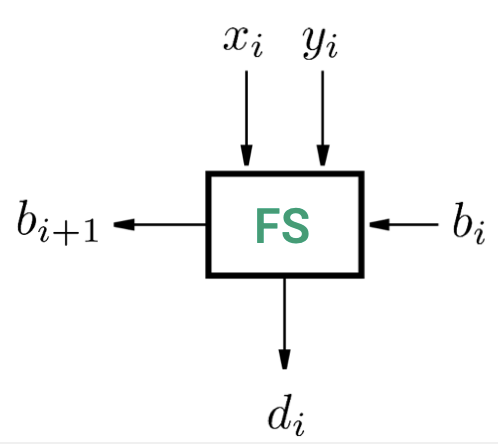
\includegraphics[width=0.60\textwidth]{circuits/8.2.4.png} % Replace 'path_to_image.png' with the actual path to your image file
			      		      	\end{minipage}
			      		      	  
			      		      \end{center}
			      	\end{itemize}
			      	
			      	\subsection{N-Bit Ripple-Carry Subtractor}
			      	Subtracting Two N-bit Binary Numbers
			      	
			      	Starting from the least-significant digit, we subtract pairs of digits, progressing to the most-significant digit.
			      	
			      	\begin{center}
			      		\begin{minipage}[c]{0.80\textwidth} % Adjust the width as needed for the second circuit
			      			\centering
			      			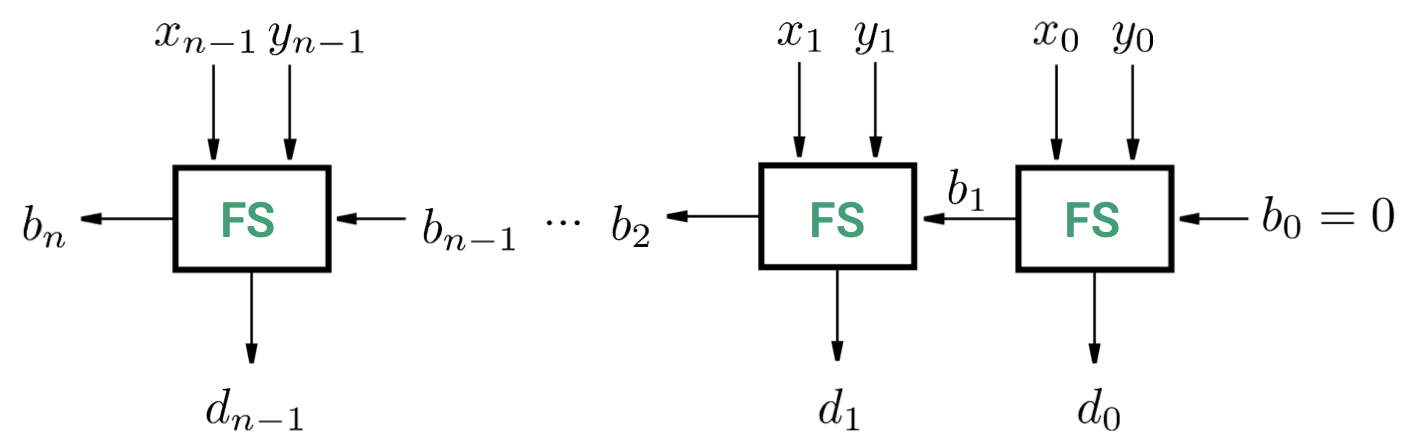
\includegraphics[width=0.70\textwidth]{circuits/8.2.5.png} % Replace 'path_to_image.png' with the actual path to your image file
			      		\end{minipage}
			      		  
			      	\end{center}
			      	
			      	\newpage
			      	\section{Adders-Subtractors in two's complement}
			      	\begin{itemize}
			      		\item[] Recall that subtracting two numbers in two's complement format requires using the two's complement of one operand:
			      		      \begin{equation*}
			      		      	X - Y = X + \overline{Y} + 1
			      		      \end{equation*}
			      		\item[] $\overline{Y}$ is obtained by complementing each of the bits of $Y$
			      		\item[] Assume a control signal $op$ determines which operation to perform \newline($op = 0$: addition, $op = 1$: subtraction)
			      	\end{itemize}
			      	  
			      	\[
			      		\begin{array}{c|c}
			      			op & f(X, Y)              \\
			      			\hline
			      			0  & X + Y                \\
			      			1  & X + \overline{Y} + 1 
			      		\end{array}
			      	\]
			      	  
			      	\[
			      		f(X, Y) = X + \overline{op} \cdot Y + op \cdot \overline{Y} + op
			      	\]
			      	
			      	\vspace*{10px}
			      	
			      	One circuit, able to perform two operations :
			      	\begin{center}
			      		\begin{minipage}[c]{0.90\textwidth} % Adjust the width as needed for the second circuit
			      			\centering
			      			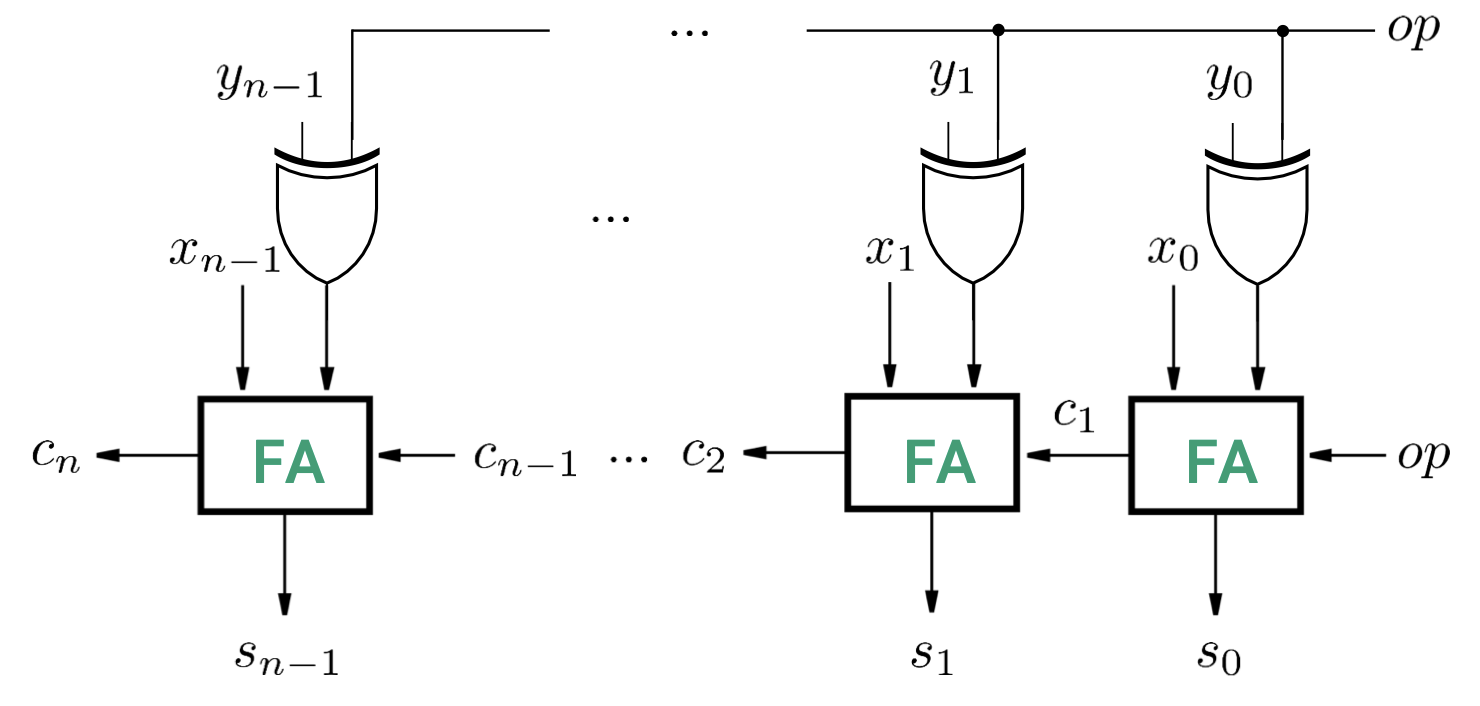
\includegraphics[width=0.90\textwidth]{circuits/8.3.png} % Replace 'path_to_image.png' with the actual path to your image file
			      		\end{minipage}
			      	\end{center}
			      	
			      	\section{Fast Adders}
			      	\subsection{Performance Matters}
			      	\begin{itemize}
			      		\item[] Addition and subtraction are essential operations in computing systems and their efficiency is crucial for overall system performance.
			      		\item[] The value of a system is quantified by the ratio of its performance to cost.
			      	\end{itemize}
			      	\[
			      		\text{value} = \frac{\text{performance}}{\text{price}}
			      	\]
			      	\subsection{Examples of delays}
			      	
			      	\subsubsection{Full Adder}
			      	\scalebox{0.8}{% Adjust <scale-factor> to your desired scaling factor, e.g., 0.9 for 90% size
			      		\begin{minipage}[c]{0.5\textwidth}
			      			\begin{itemize}
			      				\item[-] Delay to generate the sum
			      				      \begin{align*}
			      				      	t(x_i, s_i) & = t(c_i, s_i) = t(\text{XOR})        \\
			      				      	t(y_i, s_i) & = t(\text{op}, s_i) = 2t(\text{XOR}) 
			      				      \end{align*}
			      				              
			      				\item[-] Delay to generate carry-out
			      				      \begin{align*}
			      				      	t(x_i, c_{i+1}) & = t(c_i, c_{i+1}) = t(\text{AND}) + t(\text{OR})                       \\
			      				      	t(y_i, c_{i+1}) & = t(\text{op}, c_{i+1}) = t(\text{XOR}) + t(\text{AND}) + t(\text{OR}) 
			      				      \end{align*}
			      				              
			      				\item[-] Worst-case delay
			      				      \begin{align*}
			      				      	t_{\text{max}} & = \max(t(s_i), t(c_{i+1}))                                           \\
			      				      	               & = \max(2t(\text{XOR}), t(\text{XOR}) + t(\text{AND}) + t(\text{OR})) 
			      				      \end{align*}
			      				              
			      				\item[-] If all gates had equal delays:
			      				      \begin{equation*}
			      				      	t_{\text{max}} = t(c_{i+1}) = 3 \text{ Gate Delays}
			      				      \end{equation*}
			      			\end{itemize}
			      		\end{minipage}}
			      	\hfill % Adds horizontal space between the minipages
			      	\begin{minipage}[c]{0.48\textwidth} % Adjust the width as needed for the image
			      		\centering
			      		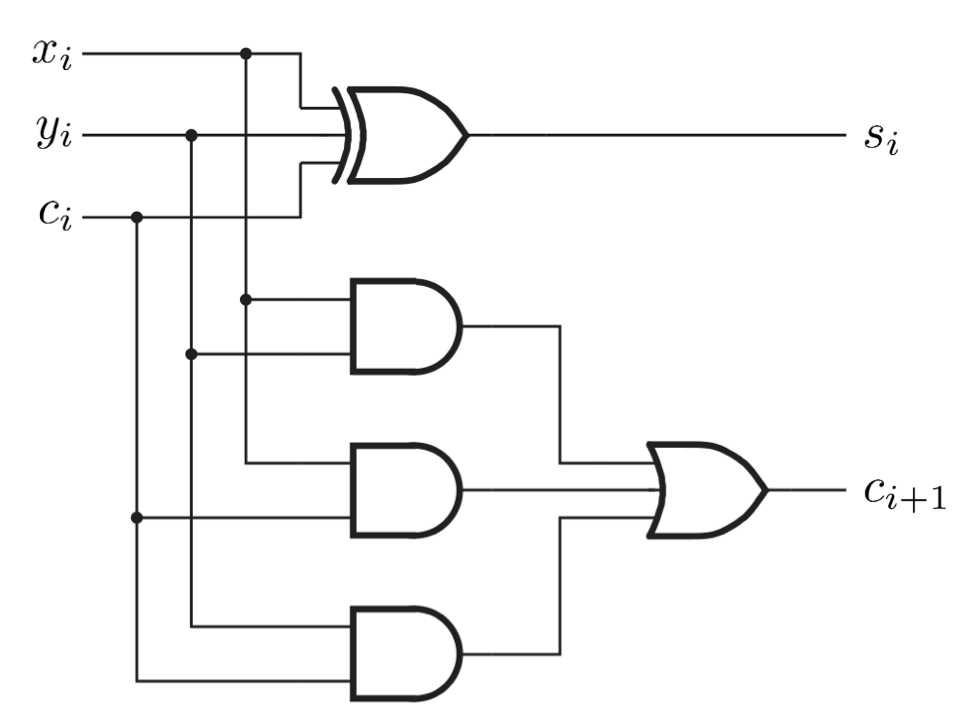
\includegraphics[width=\textwidth]{circuits/8.4.2.png} % Replace 'circuits/8.4.2.png' with the actual path to your image file
			      	\end{minipage}
			      	
			      	\subsubsection{Full Adder-Subtractor}
			      	\noindent
			      	\begin{minipage}[c]{0.45\textwidth}
			      		\scalebox{0.80}{% Change 0.8 to whatever scaling factor you need
			      			\begin{minipage}{\linewidth} % Use linewidth to scale to the minipage width
			      				\begin{itemize}
			      					\item[-] Delay to generate the sum
			      					      \begin{align*}
			      					      	t(x_i, s_i) & = t(c_i, s_i) = t(\text{XOR})        \\
			      					      	t(y_i, s_i) & = t(\text{op}, s_i) = 2t(\text{XOR}) 
			      					      \end{align*}
			      					                  
			      					\item[-] Delay to generate carry-out
			      					      \begin{align*}
			      					      	t(x_i, c_{i+1}) & = t(c_i, c_{i+1}) = t(\text{AND}) + t(\text{OR})                       \\
			      					      	t(y_i, c_{i+1}) & = t(\text{op}, c_{i+1}) = t(\text{XOR}) + t(\text{AND}) + t(\text{OR}) 
			      					      \end{align*}
			      					                  
			      					\item[-] Worst-case delay
			      					      \begin{align*}
			      					      	t_{\text{max}} & = \max(t(s_i), t(c_{i+1}))                                           \\
			      					      	               & = \max(2t(\text{XOR}), t(\text{XOR}) + t(\text{AND}) + t(\text{OR})) 
			      					      \end{align*}
			      					                  
			      					\item[-] If all gates had equal delays:
			      					      \begin{equation*}
			      					      	t_{\text{max}} = t(c_{i+1}) = 3 \text{ Gate Delays}
			      					      \end{equation*}
			      				\end{itemize}
			      			\end{minipage}
			      		}
			      	\end{minipage}
			      	\hfill
			      	\begin{minipage}[c]{0.5\textwidth}
			      		\centering
			      		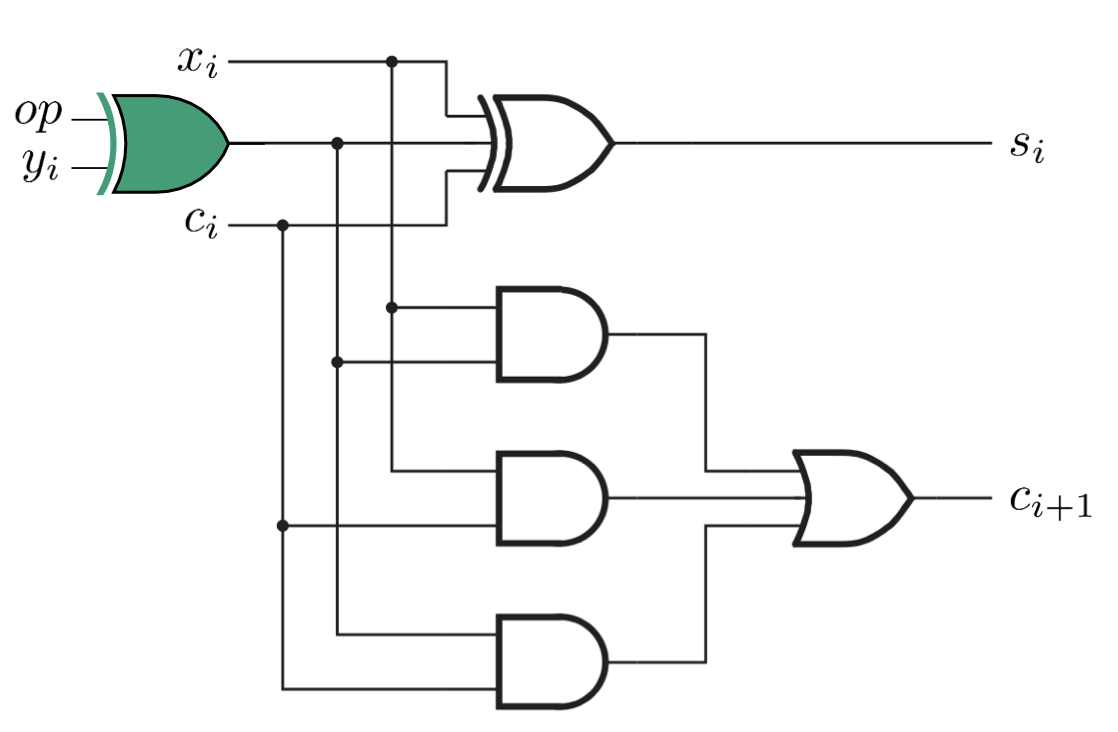
\includegraphics[width=\textwidth]{circuits/8.4.2_2.png}
			      	\end{minipage}
			      	
			      	
			      	
			      	
			      	    
			      	\newpage
			      	\subsection{Summary of the Ripple-Carry Adder-Subtractor}
			      	        
			      	The Ripple-Carry Adder-Subtractor is a fundamental component in digital circuits for performing binary addition and subtraction. The key concept to understand includes the \textbf{worst-case delay} which is pivotal in determining the efficiency of the component.
			      	        
			      	\begin{itemize}
			      		\item[-] Inputs \textbf{X}, \textbf{Y}, and \textbf{op} are immediately available, hence no delay due to waiting.
			      		\item[-] It is assumed that all gates involved have identical delay times for simplification.
			      		\item[-] The worst-case delay, also known as \textit{critical path delay (CPD)}, is crucial for assessing performance.
			      		\item[-] Given \textit{n} bits, the worst-case delay for finding the sum or difference can be calculated as \((2n + 1)\) gate delays.
			      		\item[-] While the Ripple-Carry Adder-Subtractor is a simple and effective component, it is not the most efficient in terms of speed. (With the increasing number of bits , the adder delay increases
			      		      and the computation becomes prohibitively slow)
			      	\end{itemize}
			      	\begin{center}
			      		\begin{minipage}[c]{0.90\textwidth} % Adjust the width as needed for the second circuit
			      			\centering
			      			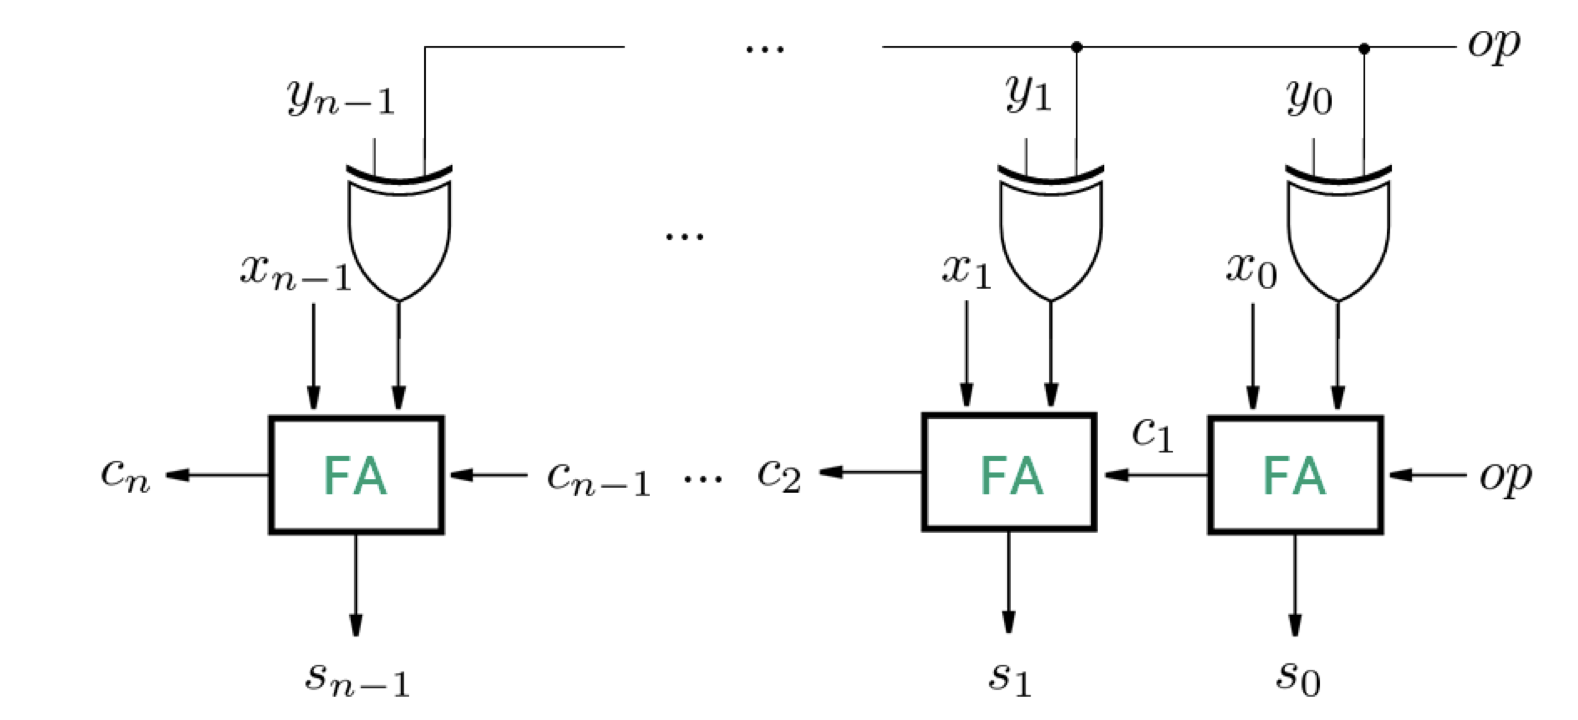
\includegraphics[width=0.90\textwidth]{circuits/8.4.3.png} % Replace 'path_to_image.png' with the actual path to your image file
			      		\end{minipage}
			      	\end{center}
			      	
			      	\newpage
			      	\subsection{Carry-Select Adder}
			      	\textit{First steps in parallel computing...}\newline
			      	In a Basic Ripple Carry Adder, the carry-in is sent to each full adder of the system until the last bit. This sequential processing of carry signals results in a significant delay, especially for large bit widths, because each full adder must wait for the carry input from its predecessor before it can complete its operation. 
			      	
			      	\vspace*{10px}
			      	A Carry Select Adder aims to fix this delay issue by improving the speed of carry propagation. It does this by having the second half of the adder calculate two sets of sums and carries for each block—once assuming the carry-in is 0, and once assuming the carry-in is 1. This is done in parallel to the operation of the first half of the adder. \newline
			      	\vspace*{10px}
			      	When the actual carry-in for the second half becomes available from the first half, a multiplexer selects the correct set of sums and carries for each block based on the actual carry-in value. This method allows the Carry Select Adder to reduce the overall computation time because it eliminates the need to wait for the carry to propagate through all the bits, significantly speeding up the addition process for multi-bit numbers.
			      	
			      	\begin{center}
			      		\begin{minipage}[c]{0.90\textwidth} % Adjust the width as needed for the second circuit
			      			\centering
			      			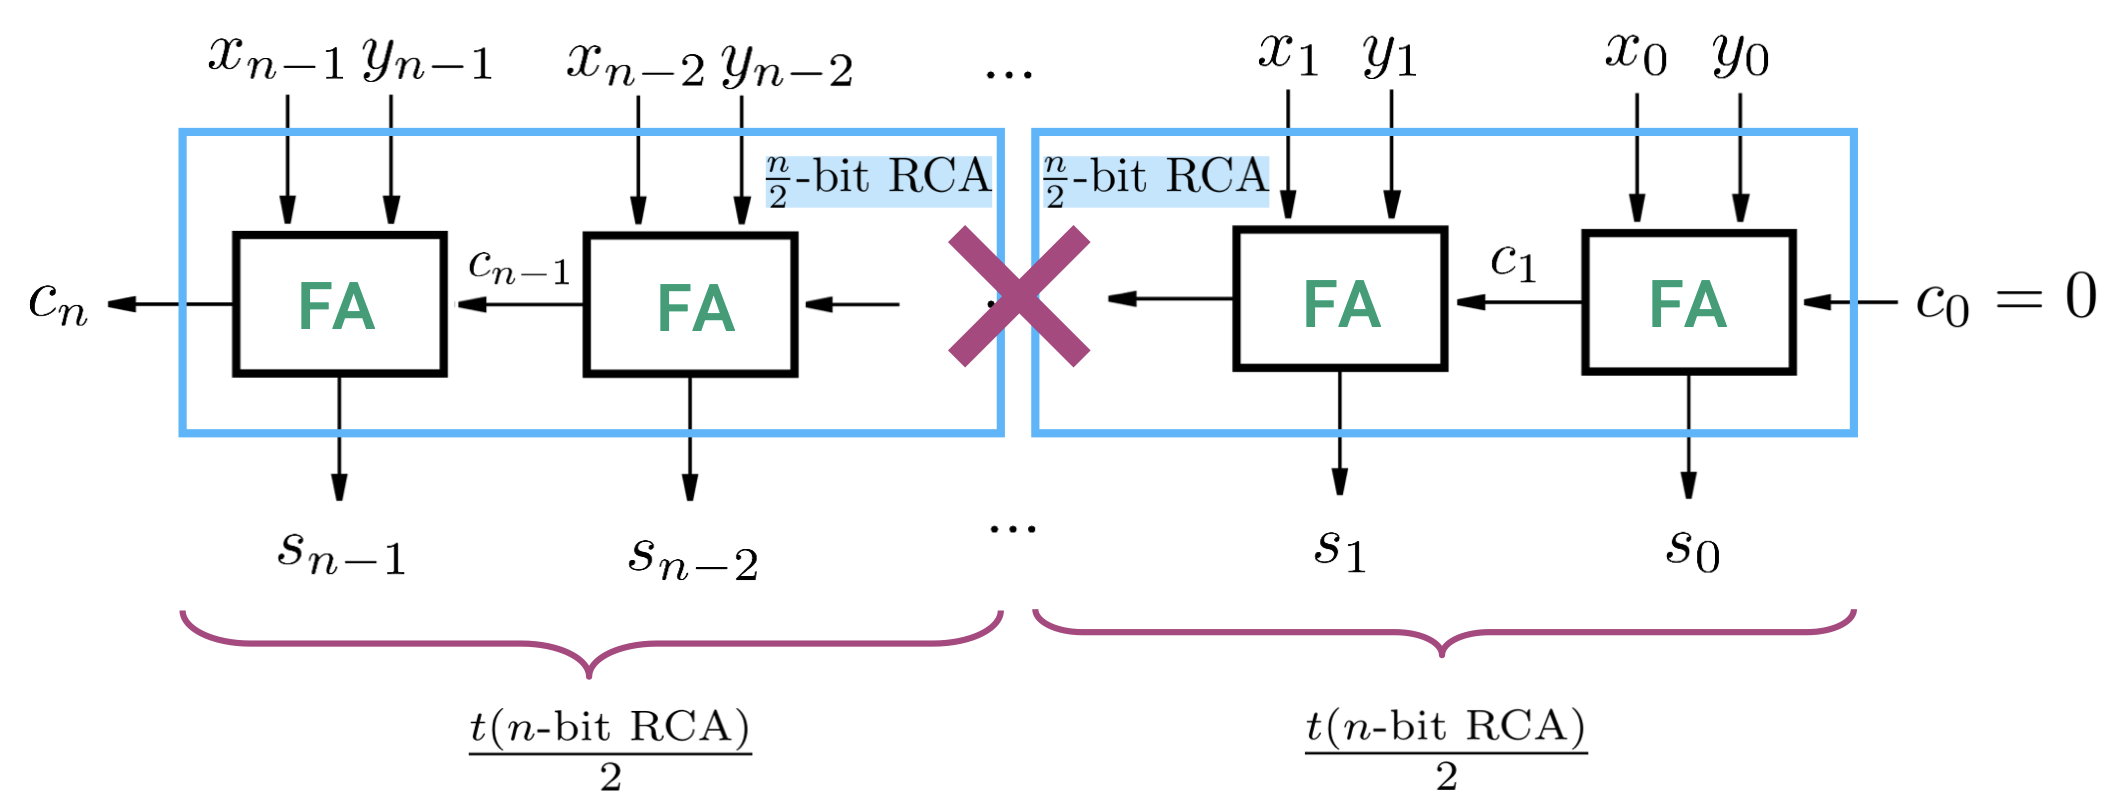
\includegraphics[width=0.90\textwidth]{circuits/8.4.4.png} % Replace 'path_to_image.png' with the actual path to your image file
			      		\end{minipage}
			      		  
			      	\end{center}
			      	
			      	\section{Shifting}
			      	\subsection{Barrel Shifter}
			      	
			      	
			      	
			      	\begin{itemize}
			      		\item[-] \textbf{Direction}: It can move bits to the left or to the right.
			      		\item[-] \textbf{Type of shift}:
			      		      \begin{itemize}
			      		      	\item[] \textit{Logical shift}: Move bits and fill the new space with zeros.
			      		      	\item[] \textit{Arithmetic shift}: Keep the sign of a binary number while shifting.
			      		      	\item[] \textit{Circular/rotation shift}: Move bits around in a circle, where the bits that fall off one end come back at the other end.
			      		      \end{itemize}
			      		\item[-] \textbf{Amount of shift}: How many places you want to move the bits (0 to n-1).
			      	\end{itemize}
			      	
			      	\newpage
			      	\subsubsection{Shift Right by one position}
			      	if $l=0$, the shift is Logical (resets the leftmost bit to 0), 
			      	if $l=x_{n-1}$, the shift is Arithmetic (conserve the sign of the number).
			      	\begin{center}
			      		\begin{minipage}[c]{0.90\textwidth} % Adjust the width as needed for the second circuit
			      			\centering
			      			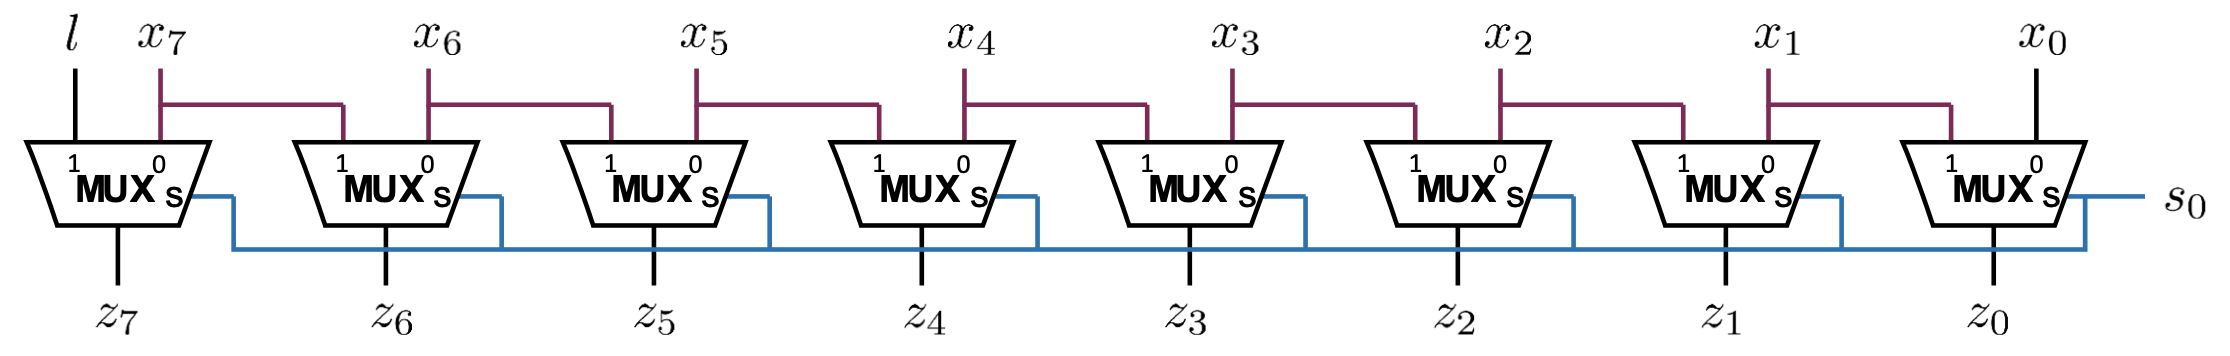
\includegraphics[width=0.90\textwidth]{circuits/8.5.1.png} % Replace 'path_to_image.png' with the actual path to your image file
			      		\end{minipage}
			      	\end{center}
			      	
			      	Thus, the corresponding truth table:
			      	\begin{table}[h]
			      		\centering
			      		\begin{tabular}{c|l}
			      			\( s_0 \) & \multicolumn{1}{c}{$z_7z_6z_5z_4z_3z_2z_1z_0$} \\ \hline
			      			0         & \( \, x_7x_6x_5x_4x_3x_2x_1x_0 \)              \\
			      			1         & \( \; \; \; lx_7x_6x_5x_4x_3x_2x_1 \)          \\
			      		\end{tabular}
			      	\end{table}
			      	\subsubsection{Shift Right by up to Three positions}
			      	
			      	
			      	
			      	\begin{center}
			      		\begin{minipage}[c]{0.90\textwidth} % Adjust the width as needed for the second circuit
			      			\centering
			      			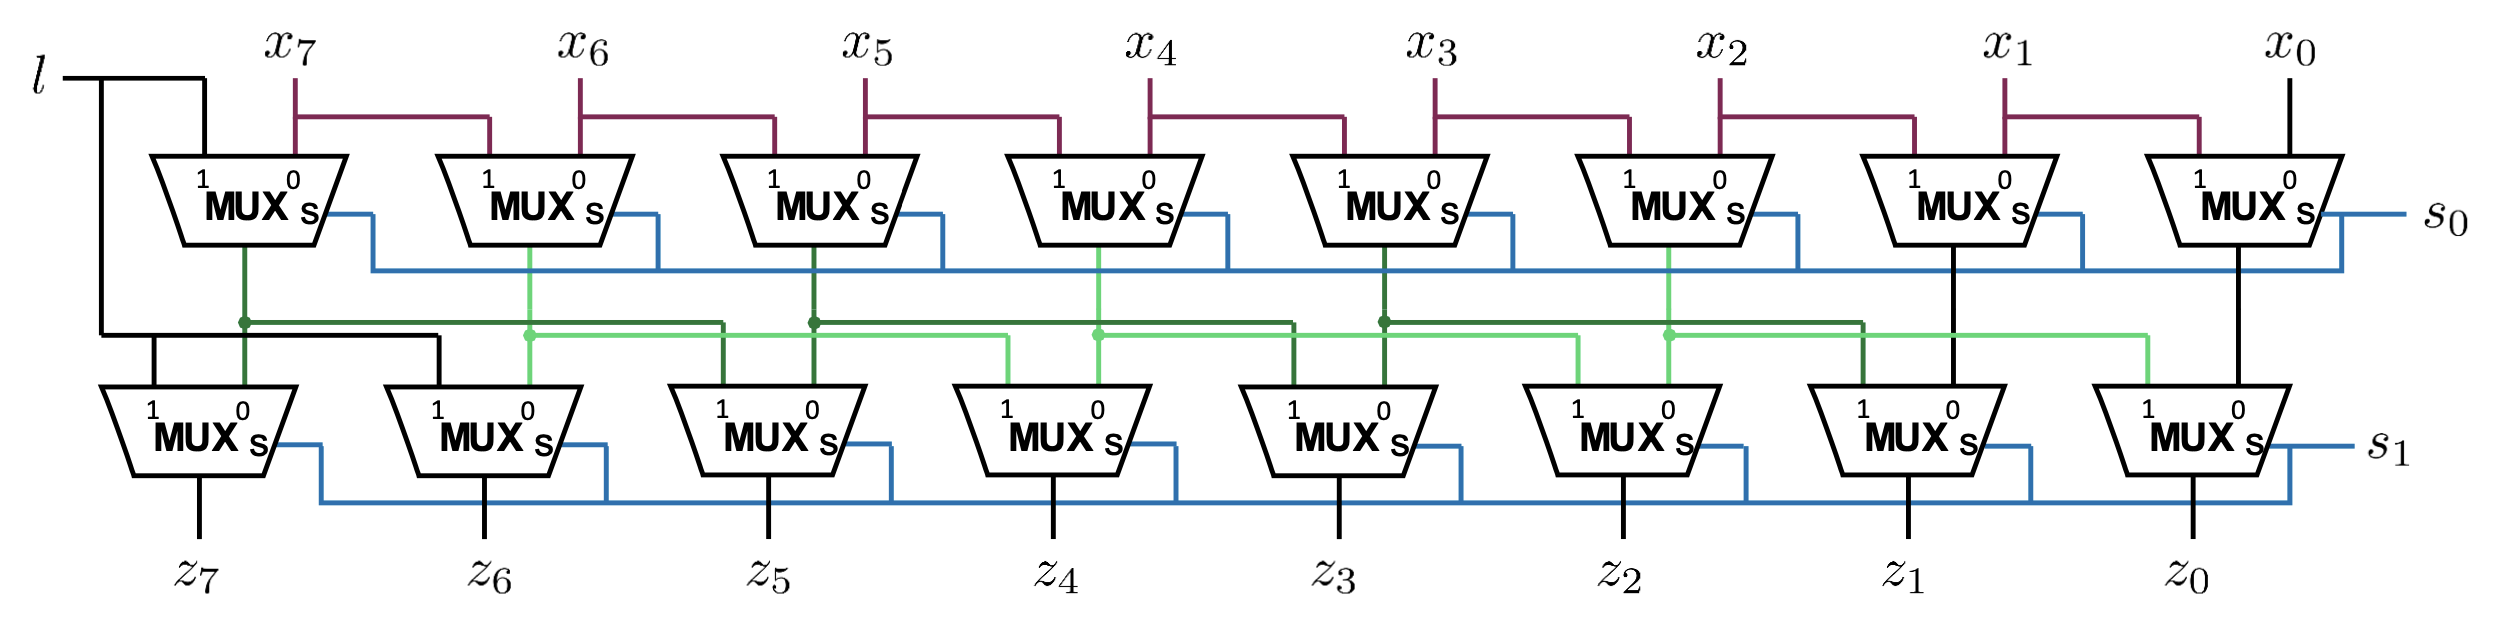
\includegraphics[width=0.90\textwidth]{circuits/8.5.1_2.png} % Replace 'path_to_image.png' with the actual path to your image file
			      		\end{minipage}
			      	\end{center}
			      	
			      	Thus, the corresponding table :
			      	\begin{table}[h]
			      		\centering
			      		\begin{tabular}{c|c||c}
			      			$s_1$ & $s_0$ & $z_7 z_6 z_5 z_4 z_3 z_2 z_1 z_0$ \\ \hline
			      			0     & 0     & $x_7 x_6 x_5 x_4 x_3 x_2 x_1 x_0$ \\
			      			0     & 1     & $l x_7 x_6 x_5 x_4 x_3 x_2 x_1$   \\
			      			1     & 0     & $ll x_7 x_6 x_5 x_4 x_3 x_2$      \\
			      			1     & 1     & $lll x_7 x_6 x_5 x_4 x_3$         \\
			      		\end{tabular}
			      	\end{table}
			      	
			      	\newpage
			      	\subsection{Bidirectional Shifting by up to 7 positions}
			      	The circuit implements a bidirectional shift register enabling shifts left or right by up to seven positions. It consists of:
			      	
			      	\begin{itemize}
			      		\item[] Inputs \texttt{in0} to \texttt{in7} and outputs \texttt{out0} to \texttt{out7}.
			      		\item[] Control signals \texttt{S0}, \texttt{S1}, \texttt{S2} for the shift magnitude, and \texttt{dir} for the direction.
			      		\item[] A logical input \texttt{l} for leftward shifts.
			      	\end{itemize}
			      	
			      	Shift operation:
			      	\begin{itemize}
			      		\item[] \textbf{Right Shift:} With \texttt{dir} high, each MUX passes the value from the left input to the right output.
			      		\item[] \textbf{Left Shift:} With \texttt{dir} low, each MUX passes the value from the right input to the left output, with \texttt{out7} taking the value of \texttt{l}.
			      		\item[] The signals \texttt{S0}, \texttt{S1}, and \texttt{S2} determine the shift amount, with binary encoding representing 0 to 7 positions.
			      	\end{itemize}
			      	
			      	
			      	The circuit (\textit{which might look a bit scary at first...}) looks like this:
			      	\begin{center}
			      		\begin{minipage}[c]{0.90\textwidth} % Adjust the width as needed for the second circuit
			      			\centering
			      			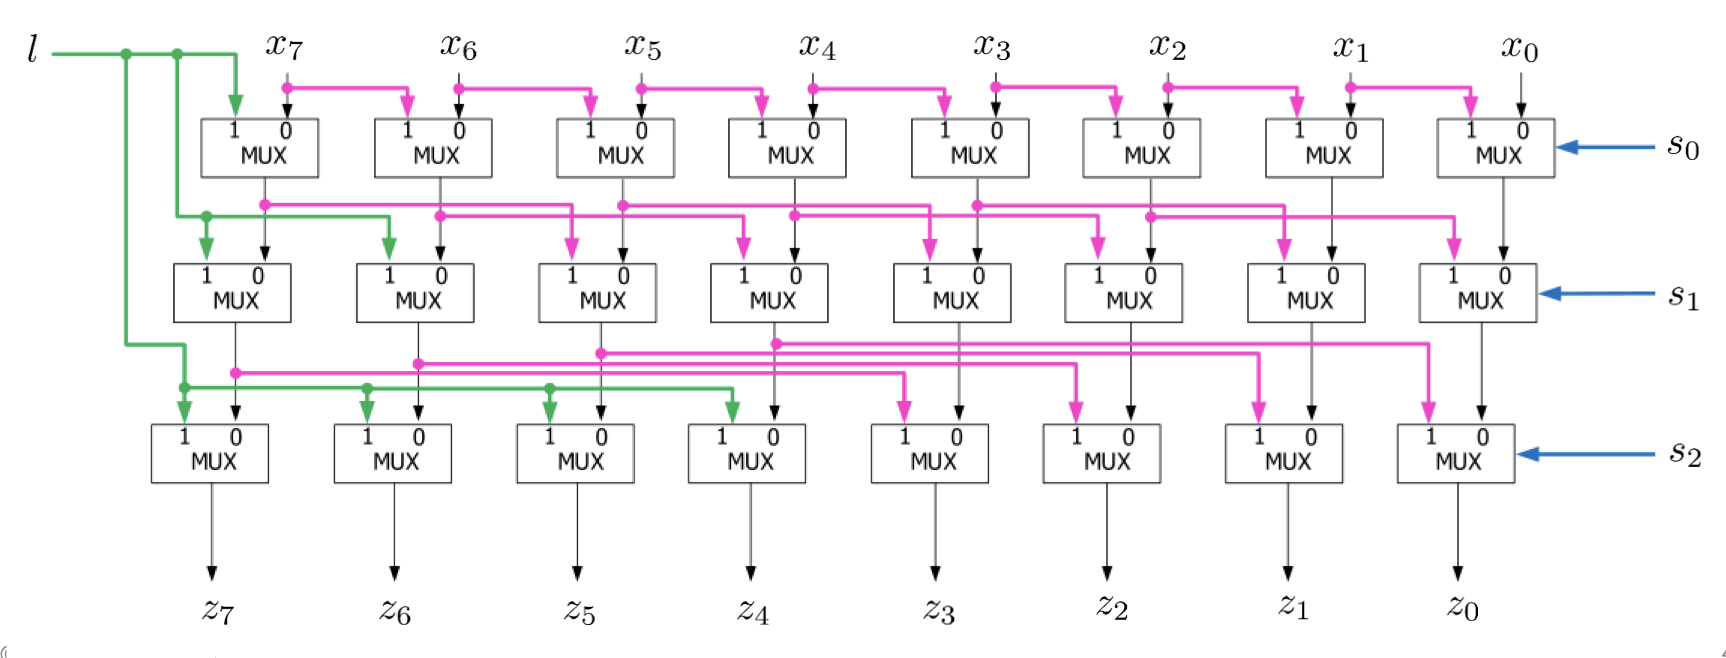
\includegraphics[width=0.90\textwidth]{circuits/8.5.2.png} 
			      		\end{minipage}
			      	\end{center}
			      	
			      	
			      	
			      	\begin{table}[h!]
			      		\centering
			      		\resizebox{240pt}{!}{% Resize table to fit the text width
			      			\begin{tabular}{cccc|l}
			      				\hline
			      				\textbf{S2} & \textbf{S1} & \textbf{S0} & \textbf{dir} & \multicolumn{1}{c}{\textbf{Operation}} \\ \hline
			      				0           & 0           & 0           & 0            & No shift (or shift by 0) to the left   \\
			      				0           & 0           & 0           & 1            & No shift (or shift by 0) to the right  \\
			      				0           & 0           & 1           & 0            & Shift 1 position to the left           \\
			      				0           & 0           & 1           & 1            & Shift 1 position to the right          \\
			      				0           & 1           & 0           & 0            & Shift 2 positions to the left          \\
			      				0           & 1           & 0           & 1            & Shift 2 positions to the right         \\
			      				0           & 1           & 1           & 0            & Shift 3 positions to the left          \\
			      				0           & 1           & 1           & 1            & Shift 3 positions to the right         \\
			      				1           & 0           & 0           & 0            & Shift 4 positions to the left          \\
			      				1           & 0           & 0           & 1            & Shift 4 positions to the right         \\
			      				1           & 0           & 1           & 0            & Shift 5 positions to the left          \\
			      				1           & 0           & 1           & 1            & Shift 5 positions to the right         \\
			      				1           & 1           & 0           & 0            & Shift 6 positions to the left          \\
			      				1           & 1           & 0           & 1            & Shift 6 positions to the right         \\
			      				1           & 1           & 1           & 0            & Shift 7 positions to the left          \\
			      				1           & 1           & 1           & 1            & Shift 7 positions to the right         \\ \hline
			      			\end{tabular}
			      		}
			      		\caption{Truth Table for the Bidirectional Shift Register}
			      		\label{tab:truth_table}
			      	\end{table}
			      	        
			      	\chapter{Digital Logic (PART IV)}
			      	
				
			      	\section{Transistors}
			      	A Metal-Oxide-Semiconductor Field-Effect Transistor (MOSFET) is a transistor used for amplifying or switching electronic signals. It has three terminals:
			      	
			      	\begin{itemize}
			      		\item[-] \textbf{Drain (D)}: Current exits the transistor, with voltage \( V_D\).
			      		\item[-] \textbf{Gate (G)}: Controls the transistor operation, with voltage \( V_G\).
			      		\item[-] \textbf{Source (S)}: Current enters the transistor, with voltage \( V_S\).
			      	\end{itemize}
			      	
			      	
			      	
			      	The gate voltage (\( V_G \)) controls the current flow between the drain and source. When \( V_G \) exceeds a certain threshold, an electric field is created that allows current to flow, making the MOSFET act as an efficient electronic switch.
			      \vspace*{20px}
					\subsection{NMOS Transistor Switches}
			      	\small NMOS works like a switch that turns on to let electricity flow when you apply a certain voltage.
			      	
			      	The digital representation of it looks like this :
			      	
			      	\begin{center}
			      		
			      		\begin{minipage}[c]{0.35\textwidth} % Adjust the width as needed for the second circuit
			      			
			      			\centering
			      			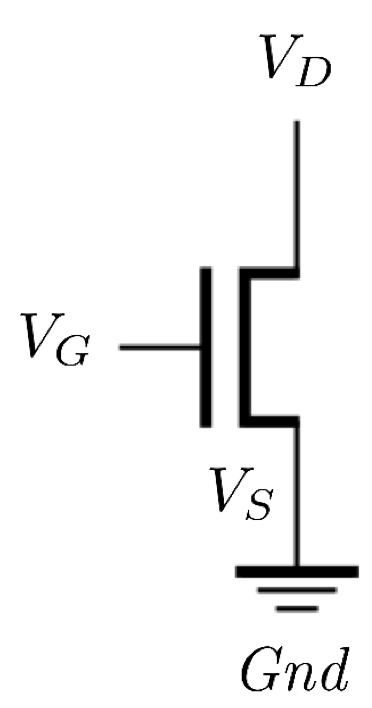
\includegraphics[width=0.35\textwidth]{circuits/9.1.1.png} 
			      		\end{minipage}
			      	\end{center}
			
			      	\begin{itemize}
			      		\item[-] Open ($x=0$); $V_{G} = 0$
			      		      \newline
			      		      \noindent\begin{minipage}{0.5\textwidth}
			      		      \begin{tikzpicture}
			      		      	\draw (0,0) -- (2,0);
			      		      	\draw (2,0) -- (2.5,0.5);
			      		      	\draw (3,0) -- (4,0);
			      		      	\filldraw [black] (2,0) circle (2pt);
			      		      	\filldraw [black] (3,0) circle (2pt);
			      		      \end{tikzpicture}
			      		\end{minipage}%
			      		\begin{minipage}{0.30\textwidth}
			      			
			      			\centering
			      			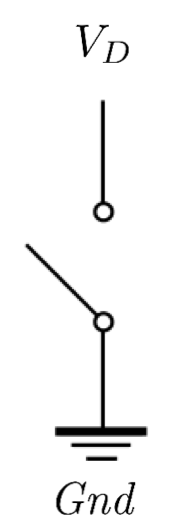
\includegraphics[width=0.3\textwidth]{circuits/9.1.1_3.png} % Replace with actual file path
			      		\end{minipage}
			      		    
			      		     
			      		\item[-] Closed ($x=1$); $V_{G} = V_{DD}$
			      		      \newline
			      		      \noindent\begin{minipage}{0.5\textwidth}
			      		      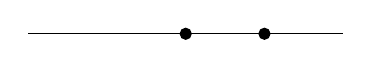
\begin{tikzpicture}
			      		      	\draw (0,0) -- (2,0);
			      		      	\draw (2,0) -- (4,0);
			      		      	\filldraw [black] (2,0) circle (2pt);
			      		      	\filldraw [black] (3,0) circle (2pt);
			      		      \end{tikzpicture}
			      		\end{minipage}%
			      		\begin{minipage}{0.30\textwidth}
			      			\centering
			      			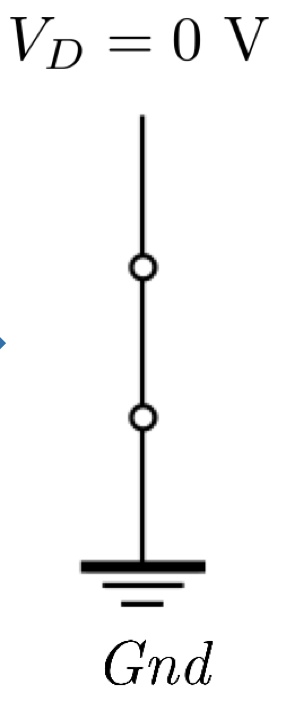
\includegraphics[width=0.30\textwidth]{circuits/9.1.1_2.png} % Replace with actual file path
			      		\end{minipage}
			      	\end{itemize}
			      	
			    
	
			      	\subsection{PMOS Transistor Switches}
			      	\textit{For french people, P like Porte, you push the door (need energy) to open it.}
			      	\newline PMOS works like a switch that turns on to let electricity flow when you apply a certain voltage.
			      	
			      	The digital representation of it looks like this :
			      	
			      	\begin{center}
			      		\begin{minipage}[c]{0.40\textwidth} % Adjust the width as needed for the second circuit
			      			\centering
			      			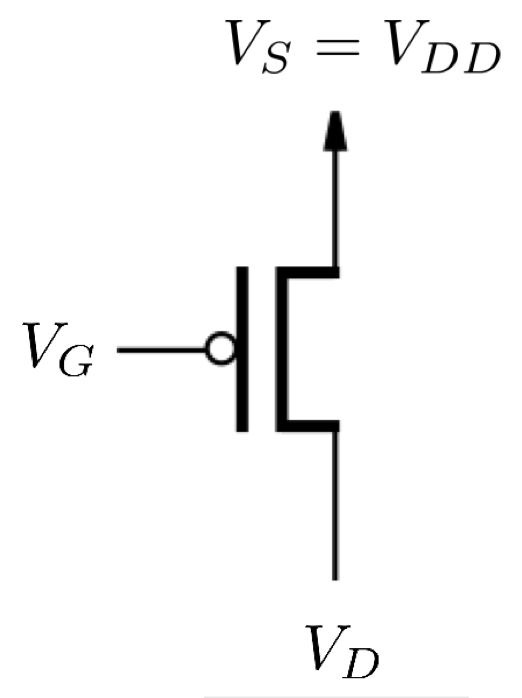
\includegraphics[width=0.40\textwidth]{circuits/9.1.2.png} 
			      		\end{minipage}
			      	\end{center}
			      	\begin{itemize}
			      		\item[-] Open ($x=1$); $V_{G} = V_{DD}$
			      		      \newline
			      		      \noindent\begin{minipage}{0.5\textwidth}
			      		      \begin{tikzpicture}
			      		      	\draw (0,0) -- (2,0);
			      		      	\draw (2,0) -- (2.5,0.5);
			      		      	\draw (3,0) -- (4,0);
			      		      	\filldraw [black] (2,0) circle (2pt);
			      		      	\filldraw [black] (3,0) circle (2pt);
			      		      \end{tikzpicture}
			      		\end{minipage}%
			      		\begin{minipage}{0.30\textwidth}
			      			\centering
			      			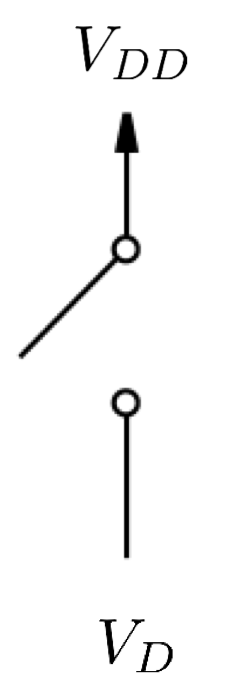
\includegraphics[width=0.3\textwidth]{circuits/9.1.2_2.png} % Replace with actual file path
			      		\end{minipage}
			      		    
			      		     
			      		\item[-] Closed ($x=0$); $V_{G} = 0$
			      		      \newline
			      		      \noindent\begin{minipage}{0.5\textwidth}
			      		      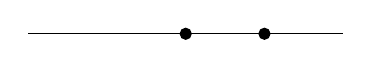
\begin{tikzpicture}
			      		      	\draw (0,0) -- (2,0);
			      		      	\draw (2,0) -- (4,0);
			      		      	\filldraw [black] (2,0) circle (2pt);
			      		      	\filldraw [black] (3,0) circle (2pt);
			      		      \end{tikzpicture}
			      		\end{minipage}%
			      		\begin{minipage}{0.40\textwidth}
			      			\centering
			      			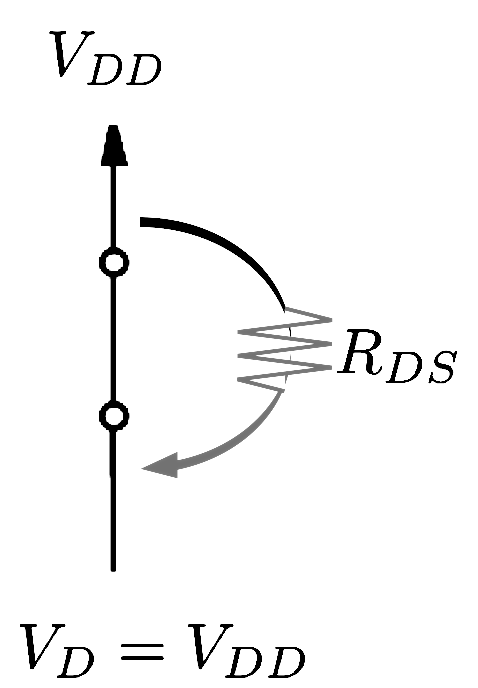
\includegraphics[width=0.40\textwidth]{circuits/9.1.2_3.png} % Replace with actual file path
			      		\end{minipage}
			      	\end{itemize}
			      	    
			      	
			      	\newpage
			      	\subsection{Example - CMOS}
			      	\begin{minipage}{0.5\textwidth}
			      		\begin{itemize}
			      			\item[] PMOS (T1) is connected from power supply \( V_{DD} \) to the output \( V_f \).
			      			\item[] NMOS (T2) is connected from ground to the output \( V_f \).
			      			\item[] The input voltage \( V_x \) controls the gates of both transistors.
			      		\end{itemize}
			      	\end{minipage}
			      	\begin{minipage}{0.50\textwidth}
			      		\centering
			      		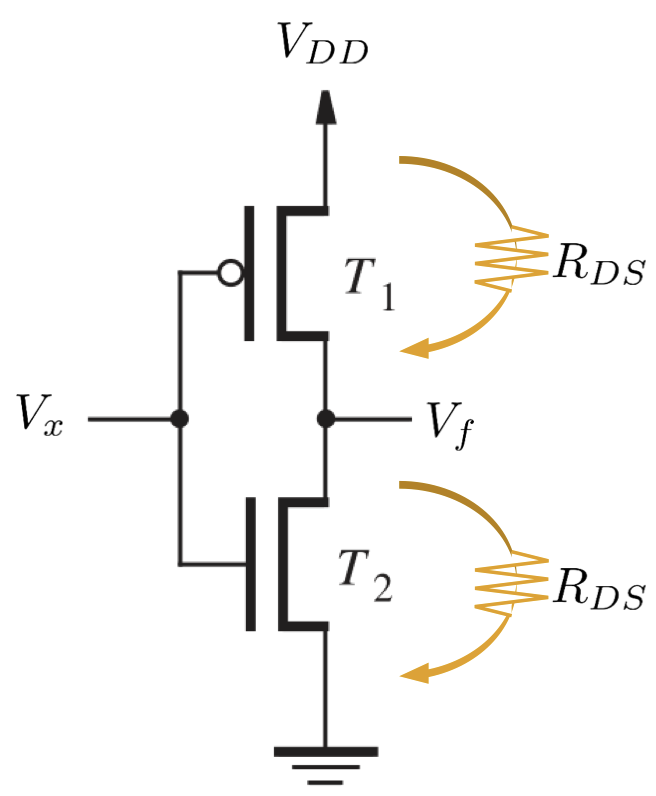
\includegraphics[width=0.60\textwidth]{circuits/9.1.3.png} % Replace with actual file path
			      	\end{minipage}
			      	            
			      	  
			      	\vspace*{20px}
			      	
			      	When \( V_x \) is low:
			      	\begin{itemize}
			      		\item[-] T1 conducts (on) since PMOS is active when gate voltage is less than the source.
			      		\item[-] T2 does not conduct (off) as NMOS requires gate voltage higher than the source to be active.
			      		\item[-] Thus, \( V_f \) is connected to \( V_{DD} \), resulting in a high output (logical '1').
			      	\end{itemize}
			      	  
			      	When \( V_x \) is high:
			      	\begin{itemize}
			      		\item[-] T1 does not conduct (off).
			      		\item[-] T2 conducts (on).
			      		\item[-] Consequently, \( V_f \) is pulled to ground, producing a low output (logical '0').
			      	\end{itemize}
			      	  
			      	CMOS circuits are power efficient as they draw significant power only during the transition between states (dynamic power consumption), not while in a steady state.
			      	  
			      	\vspace*{10px}
			      	
			      	Thus, the truth table:
			      	\begin{figure}[h]
			      		\centering
			      		\begin{tabular}{c|c|c|c}
			      			\( x \) & \( T_1 \) & \( T_2 \) & \( f \) \\
			      			\hline
			      			0       & ON        & OFF       & 1       \\
			      			1       & OFF       & ON        & 0       \\
			      		\end{tabular}
			      	\end{figure}
			      	
			      	
			      	\textbf{The circuit opperates as an inverter. } \textit{(NOT GATE)}
			      	
			      	\newpage
			      	\subsection{CMOS Circuit Structure}
			      	\begin{figure}[h]
			      		\centering
			      		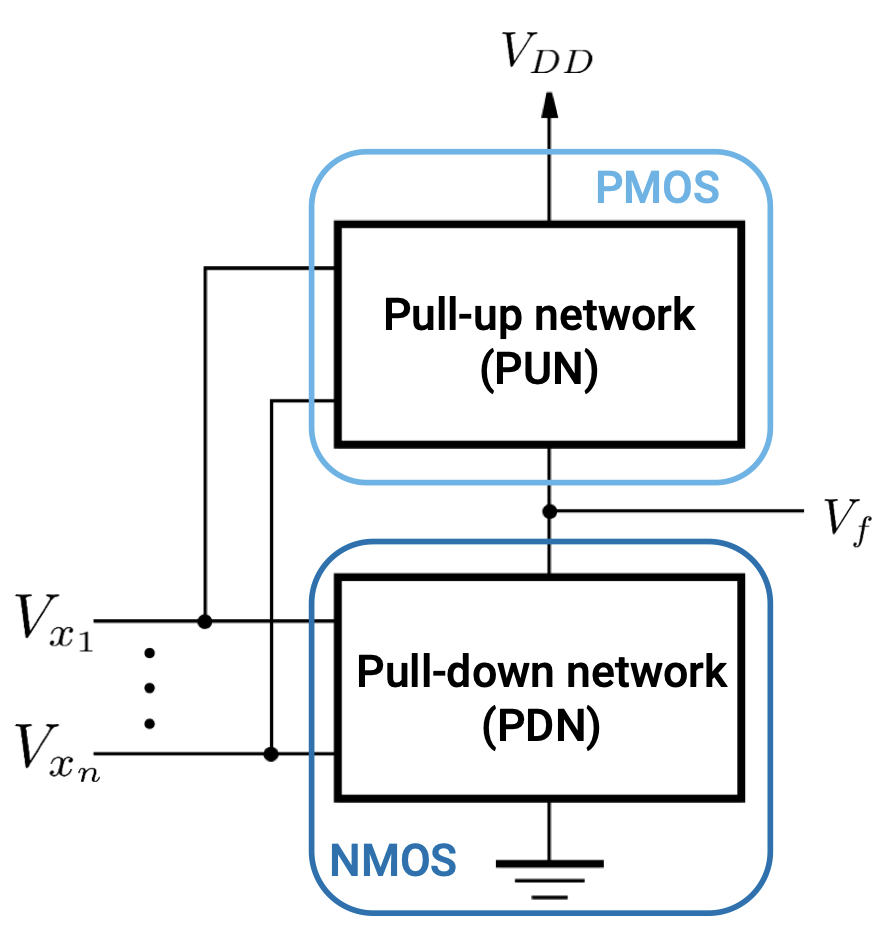
\includegraphics[width=0.4\textwidth]{circuits/9.1.4.png} % Replace with the actual path to the image
			      	\end{figure}
			      	
			      	\begin{itemize}
			      		\item[] Complementary functions performed by a pull-up and pull-down network:
			      		      \begin{itemize}
			      		      	\item[-] Pull-up composed of \textbf{PMOS}
			      		      	\item[-] Pull-down composed of \textbf{NMOS}
			      		      \end{itemize}
			      		\item[] Pull-up and pull-down networks are \textit{dual} to one another and have an \textit{equal} number of transistors
			      	\end{itemize}
			      	
			      	\subsection{CMOS Circuits - Examples}
			      	\textit{Personal Remark. Make sure you're able to quickly identify NMOS and PMOS and how they work as this really helps understanding how we construct the table for more complex CMOS circuits}
			      	\subsubsection{NOR Gate}
			      	\begin{figure}[h]
			      		\centering
			      		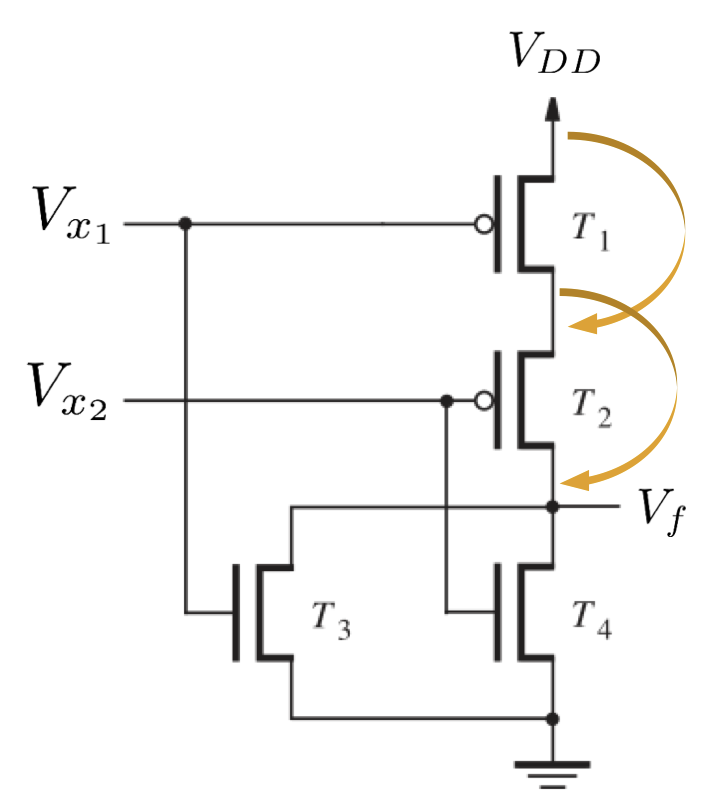
\includegraphics[width=0.3\textwidth]{circuits/9.1.5.png} % Replace with the actual path to the image
			      	\end{figure}
			      	Thus the truth table: 
			      	\begin{center}
			      		\begin{tabular}{ |c|c||c|c|c|c||c| }
			      			\hline
			      			\( x_1 \) & \( x_2 \) & \( T_1 \) & \( T_2 \) & \( T_3 \) & \( T_4 \) & \( V_f \) \\
			      			\hline
			      			0         & 0         & ON        & ON        & OFF       & OFF       & 1         \\
			      			0         & 1         & ON        & OFF       & OFF       & ON        & 0         \\
			      			1         & 0         & OFF       & ON        & ON        & OFF       & 0         \\
			      			1         & 1         & OFF       & OFF       & ON        & ON        & 0         \\
			      			\hline
			      		\end{tabular}
			      	\end{center}
			      	
			      	Cost (size, area): four transistors
			      	
			      	\subsubsection{NAND Gate}
			      	\begin{itemize}
			      		\item Find the functionality of the given CMOS gate
			      	\end{itemize}
			      	      
			      	\begin{figure}[h]
			      		\centering
			      		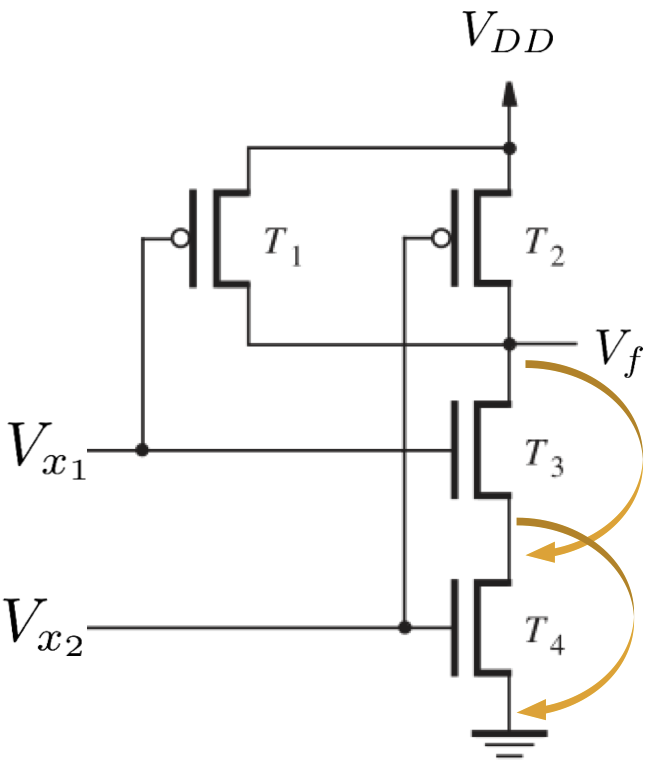
\includegraphics[width=0.3\textwidth]{circuits/9.1.5_2.png} % Replace with the actual path to the image
			      	\end{figure}
			      	      
			      	
			      	Thus the truth table: 
			      	\begin{center}
			      		\begin{tabular}{ |c|c||c|c|c|c||c| }
			      			\hline
			      			\( x_1 \) & \( x_2 \) & \( T_1 \) & \( T_2 \) & \( T_3 \) & \( T_4 \) & \( f \) \\
			      			\hline
			      			0         & 0         & ON        & ON        & OFF       & OFF       & 1       \\
			      			0         & 1         & ON        & OFF       & OFF       & ON        & 1       \\
			      			1         & 0         & OFF       & ON        & ON        & OFF       & 1       \\
			      			1         & 1         & OFF       & OFF       & ON        & ON        & 0       \\
			      			\hline
			      		\end{tabular}
			      	\end{center}
			      	      
			      	Cost (size, area): four transistors
			      	
			      	\subsubsection{AND Gate}
			      	A NAND gate (green) followed by a NOT (blue) gate, forming an AND gate.
			      	\begin{figure}[h]
			      		\centering
			      		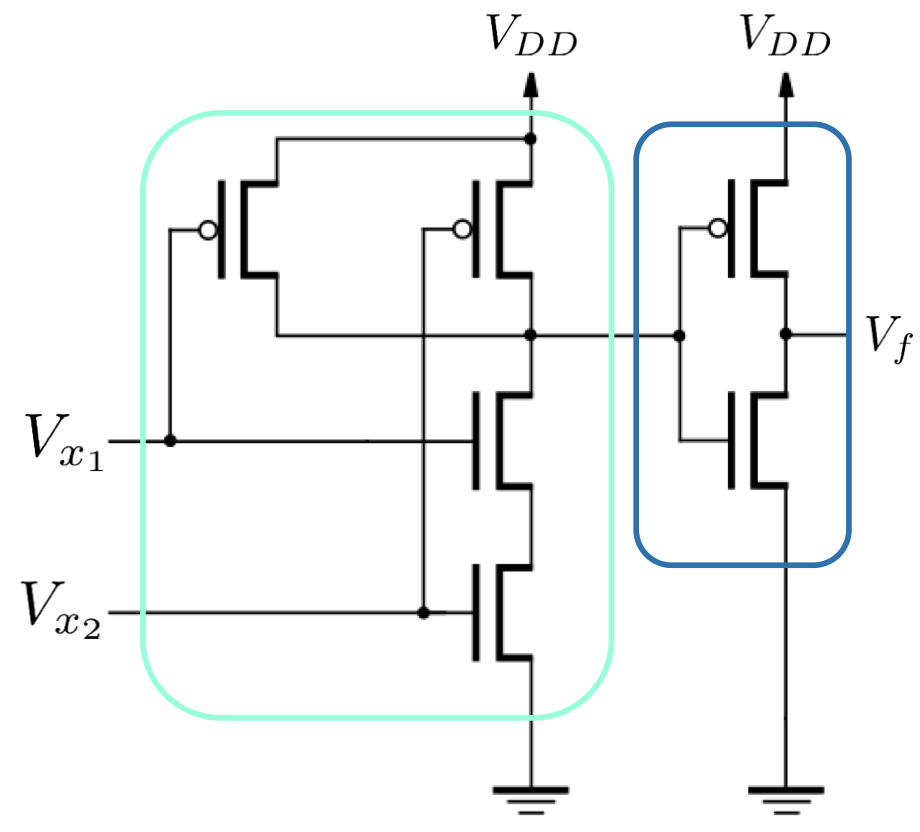
\includegraphics[width=0.3\textwidth]{circuits/9.1.5_3.png}
			      	\end{figure}
			      	        
			      	Thus the truth table:
			      	        
			      	\begin{center}
			      		\begin{tabular}{cc|c}
			      			\hline
			      			\( x_1 \) & \( x_2 \) & \( f \) \\
			      			\hline
			      			0         & 0         & 0       \\
			      			0         & 1         & 0       \\
			      			1         & 0         & 0       \\
			      			1         & 1         & 1       \\
			      			\hline
			      		\end{tabular}
			      	\end{center}
			      	        
			      	Cost (size, area): six transistors
			      	
			      	
			      	\section{Real Voltage Waveforms}
			      	\subsection{Logic Values as Voltage Levels}
			      	\vspace*{5px}
			      	
			      	\begin{minipage}{0.65\textwidth}
			      		\begin{itemize}
			      			\item[] Binary values (0, 1) in digital circuits are represented as voltage levels
			      			      \begin{itemize}
			      			      	\item 0: low (voltage)
			      			      	\item 1: high (voltage)
			      			      \end{itemize}
			      			\item[] Thresholds:
			      			      \begin{itemize}
			      			      	\item {$V_{0,\text{max}}$}, the max voltage level that the circuit must interpret as \textit{low}
			      			      	\item {$V_{1,\text{min}}$}, the min voltage level that the circuit must interpret as \textit{high}
			      			      \end{itemize}
			      			\item[] Exact threshold values depend on the technology; typically:
			      			      \begin{itemize}
			      			      	\item $V_{0,\text{max}} \approx 0.4V_{DD}$
			      			      	\item $V_{1,\text{min}} \approx 0.6V_{DD}$
			      			      \end{itemize}
			      			\item[] Range $(V_{0,\text{max}}, V_{1,\text{min}})$ is undefined
			      			      \begin{itemize}
			      			      	\item Logic signals take those intermediate voltage values only while transitioning from one logic value to another.
			      			      \end{itemize}
			      		\end{itemize}
			      	\end{minipage}
			      	\hspace*{50px}
			      	\begin{minipage}{1.5\textwidth}
			      		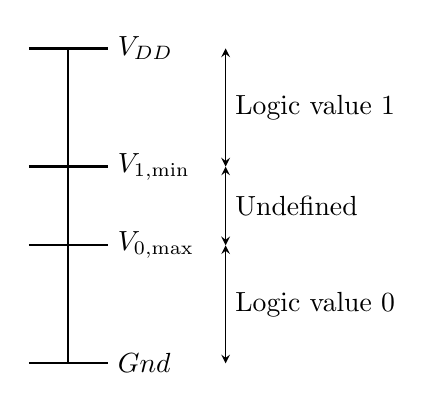
\begin{tikzpicture}
			      			% Define the coordinates for the vertical lines
			      			\coordinate (VDD) at (0,4);
			      			\coordinate (V1min) at (0,2.5);
			      			\coordinate (V0max) at (0,1.5);
			      			\coordinate (GND) at (0,0);
			      			    
			      			% Draw the vertical lines
			      			\draw[thick] (VDD) -- (GND);
			      			    
			      			% Draw the horizontal lines and labels on the left
			      			\draw[thick] (-0.5,4) -- (0.5,4) node[right] {$V_{DD}$};
			      			\draw[thick] (-0.5,2.5) -- (0.5,2.5) node[right] {$V_{1,\text{min}}$};
			      			\draw[thick] (-0.5,1.5) -- (0.5,1.5) node[right] {$V_{0,\text{max}}$};
			      			\draw[thick] (-0.5,0) -- (0.5,0) node[right] {$Gnd$};
			      			    
			      			% Draw the horizontal lines and labels on the right
			      			\draw[<->, >=stealth] (2,4) -- (2,2.5) node[midway, right] {Logic value 1};
			      			\draw[<->, >=stealth] (2,2.5) -- (2,1.5) node[midway, right] {Undefined};
			      			\draw[<->, >=stealth] (2,1.5) -- (2,0) node[midway, right] {Logic value 0};
			      		\end{tikzpicture}
			      	\end{minipage}
			      	
			      	\newpage
			      	\section{Voltage Transfer Characteristic}
			      	\subsection{CMOS Inverter (NOT gate)}
			      	
			      	The input-output voltage relationship in a real CMOS inverter is summarized by the voltage transfer characteristic.
			      	
			      	When the slope of the curve is \(-1\), we have:
			      	\begin{itemize}
			      		\item[-] the maximum input voltage that the inverter will interpret as low
			      		\item[-] the minimum input voltage that the inverter will interpret as high
			      	\end{itemize}
			      	
			      	\begin{figure}[h]
			      		\centering
			      		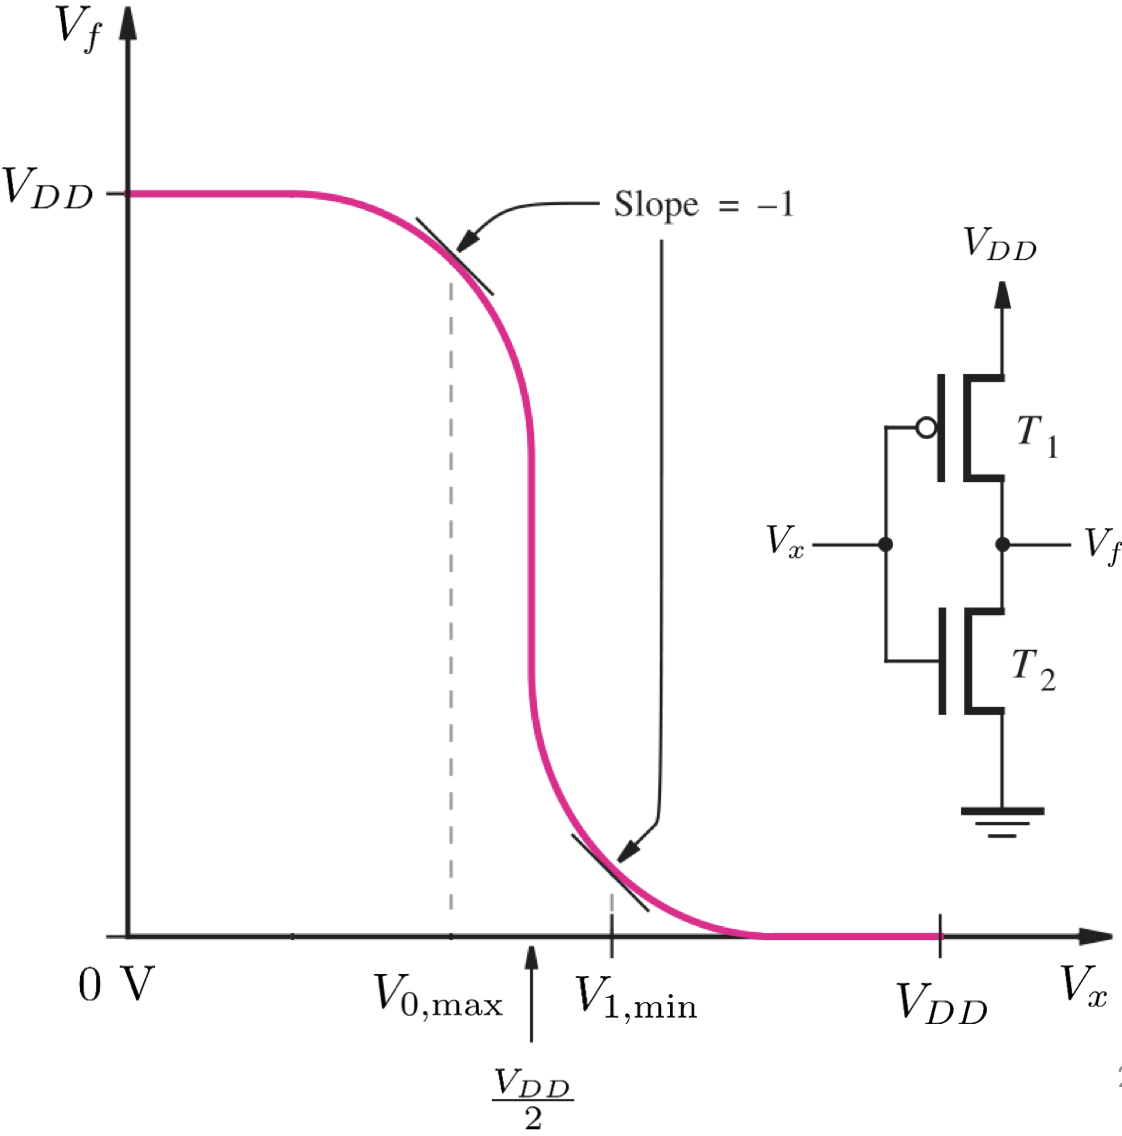
\includegraphics[width=0.5\textwidth]{circuits/9.3.1.png} 
			      		\label{fig:voltage_transfer}
			      	\end{figure}
			      	
			      	\subsection{Ideal Waveforms and Real Waveforms}
			      	Until now, we have considered ideal waveforms in digital circuits like such :
			      	
			      	\begin{center}
			      		    
			      		
			      		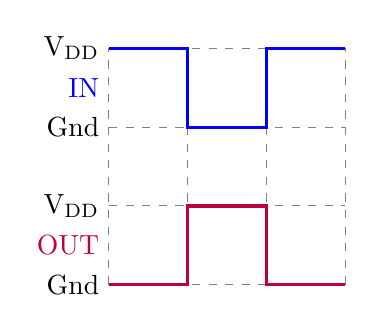
\begin{tikzpicture}
			      			% Grid
			      			\draw[dashed, gray] (0,0) grid [step=1cm] (3,3);
			      			  
			      			% Labels
			      			\node [left] at (0,3) {V\textsubscript{DD}};
			      			\node [left] at (0,2) {Gnd};
			      			\node [left] at (0,1) {V\textsubscript{DD}};
			      			\node [left] at (0,0) {Gnd};
			      			  
			      			% IN signal
			      			\draw[very thick, blue] (0,3) -- (1,3) -- (1,2) -- (2,2) -- (2,3) -- (3,3);
			      			\node [above left, blue] at (0,2.25) {IN};
			      			  
			      			% OUT signal
			      			\draw[very thick, purple] (0,0) -- (1,0) -- (1,1) -- (2,1) -- (2,0) -- (3,0);
			      			\node [below left, purple] at (0,0.75) {OUT};
			      		\end{tikzpicture}
			      	\end{center}
			      	
			      	\newpage
			      	In real gates, the transition delay between GND and V\textsubscript{DD} is not instantaneous.
			      	Also, the output is not produced instantaneously, there is a \textbf{propagation delay}.
			      	
			      	\vspace*{10px}
			      	For example, let's consider the Real Waveform of a NOT gate:
			      	\begin{figure}[h]
			      		\centering
			      		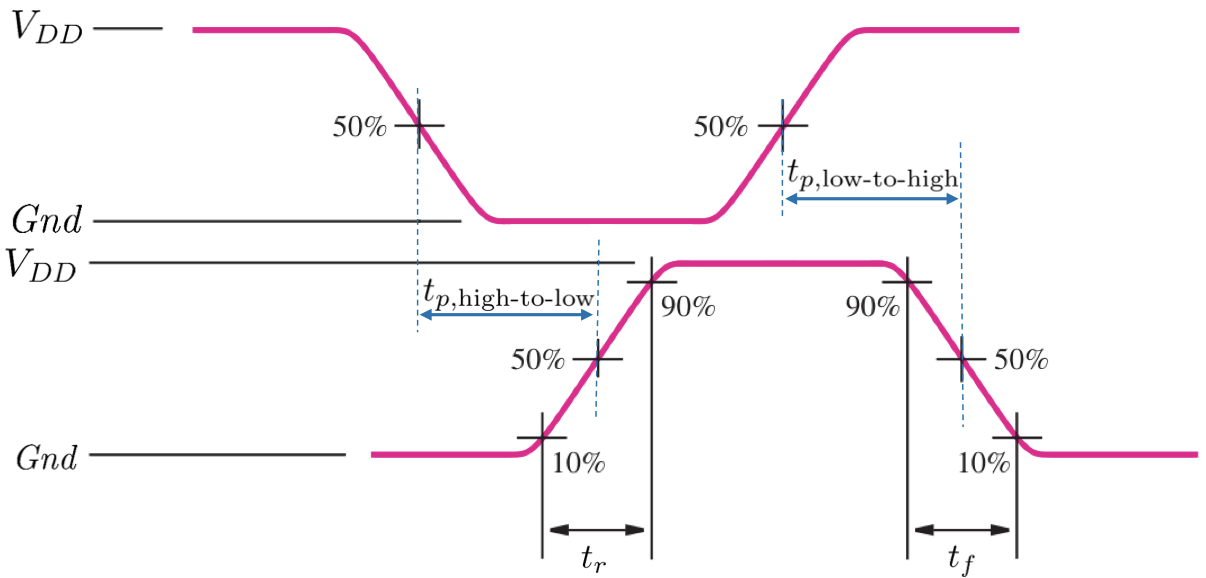
\includegraphics[width=0.8\textwidth]{circuits/9.3.2.png} 
			      	\end{figure}
			      	
			      	With $t_r$ the rise time, $t_f$ the fall time, $t_{p,high-to-low}$ the propagation delay from high to low, and $t_{p,low-to-high}$ the propagation delay from low to high. \newline
			      	
			      	Propagation delay $t_p$ is the time when the voltage is at 50\% of the $V_{DD}$.\newline 
			      	\textbf{In general, $t_{p,high-to-low} \neq t_{p,low-to-high}$} \newline
			      	\newpage
			      	\section{Dynamic Operation}
			      	
			      	In digital circuits, the operation and performance significantly depend on various factors like the design's ability to handle multiple inputs and outputs, as well as the inherent physical properties of the components used. 
			      	
			      	\subsection{Fan-In and Fan-Out}
			      	
			      	\textbf{Fan-In} refers to the maximum number of inputs a gate can handle. \textit{eg. $fan\minidash{}in(AND) = 2$}
			      	\vspace{10px}
			      	\newline
			      	\textbf{Fan-Out} refers to the maximum number of gates a gate can drive. \textit{eg. $fan\minidash{}out(NOT) = 1$}
			      	
			      	\subsection{Parasitic Capacitance}
			      	
			      	Parasitic capacitance refers to the unintended and inevitable capacitance present in transistor gates, termed as \textbf{gate parasitic capacitance} (this is like unwanted electrical 'baggage' that transistors carry which can slow things down and waste energy).
			      	\vskip 0.1in
			      	When multiple transistors connect to a single logic gate input, their individual parasitic capacitances combine to form an overall \textbf{equivalent per-input capacitance} \(C_{IN}\) (think of this as the total extra load the logic gate has to deal with). This combined capacitance:
			      	
			      	\vspace*{10px}
			      	The load capacitance (\(C_{LOAD}\)) that a logic gate must drive is equal to the input capacitance (\(C_{IN}\)) of the next gate it's connected to, meaning one gate's output has to push against the next gate's inherent electrical resistance to change its state.
			      	\begin{itemize}
			      		\item[] Acts as a load (an electrical burden) on the gate that is outputting a signal to this input, affecting its performance.
			      	\end{itemize}
			      	
			      	The equivalent capacitance at a logic gate's input, denoted $C_{IN}$, is the aggregate of parasitic capacitances from all transistor gates connected to it. This capacitance directly impacts the circuit's speed.
			      	\vskip 0.1in
			      	
			      	For example, 
			      	we've seen that a NOT gate is a CMOS circuit with an NMOS and PMOS transistor. Thus, the parasitic capacitance of the NOT gate is the sum of the parasitic capacitance of the NMOS and PMOS transistors.
			      	\subsubsection{Capacitive Effects and Circuit Speed}
			      	
			      	\begin{itemize}
			      		\item[] \textbf{Charging a Capacitor:} The voltage across a capacitor, $V_c(t)$, during charging follows the equation:
			      		      \[ V_c(t) = V_{DD}(1 - e^{-\frac{t}{RC}}) \]
			      		      where $V_{DD}$ is the supply voltage, $R$ is the resistance, and $C$ is the capacitance.
			      		          
			      		\item[] \textbf{Discharging a Capacitor:} Conversely, during discharging, the voltage decays according to:
			      		      \[ V_c(t) = V_{DD}e^{-\frac{t}{RC}} \]
			      	\end{itemize}
			      	The speed of a circuit is inversely related to the fan-out, as higher loads increase the charging time of these parasitic capacitors.
			      	
			      	\subsection{Power Dissipation}
			      	
			      	We calculate $E_c$ the energy dissipated by the circuits and $P_D$ the power dissipated by the circuits as follows:
			      	\begin{equation}
			      		E_{total} = E_{charge} + E_{discharge} = 2 \cdot \frac{1}{2}CV^2 = CV^2
			      	\end{equation}
			      	\begin{equation}
			      		P_D = fCV^2
			      	\end{equation}
			      	where $f$ represents the switching frequency, $C$ the capacitance, and $V$ the voltage. 
			      	
			      	\section{Hazards in Digital Circuits}
			      	
			      	Hazards are unintended behaviors in digital circuits that can lead to errors in operation:
			      	\begin{itemize}
			      		\item[] \textbf{Static Hazard:} Occurs when a signal unexpectedly changes levels momentarily, despite being intended to remain constant.
			      		\item[] 
			      		      \begin{center}
                                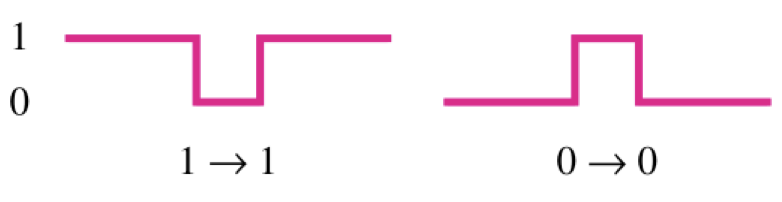
\includegraphics[width=0.3\textwidth]{circuits/9.5.png}

                              \end{center}
			      		             
			      		        
        
			      		\item[] \textbf{Dynamic Hazard:} occurs
			      		      when a signal is supposed to
			      		      change: 1\;→\;0 or 0\;→\;1, occurs if such a change
			      		      involves a short oscillation before
			      		      the signal settles into its new level.
			      		\item[] 
			      		      \centering
			      		      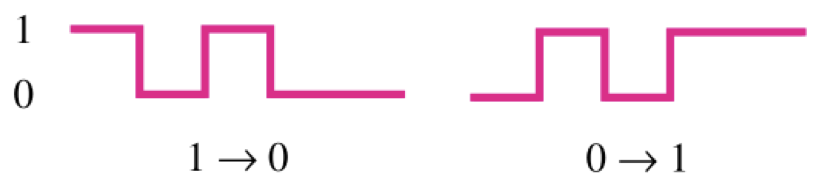
\includegraphics[width=0.3\textwidth]{circuits/9.5_1.png}
			      	\end{itemize}
			      	
			      	\chapter{Digital Logic and Verilog (PART V)}
			      	
			      	\section{CAD Design Flow}
			      	The CAD design process encompasses several critical steps, ensuring the accurate realization of digital circuits. 
			      	
			      	\begin{center}
			      		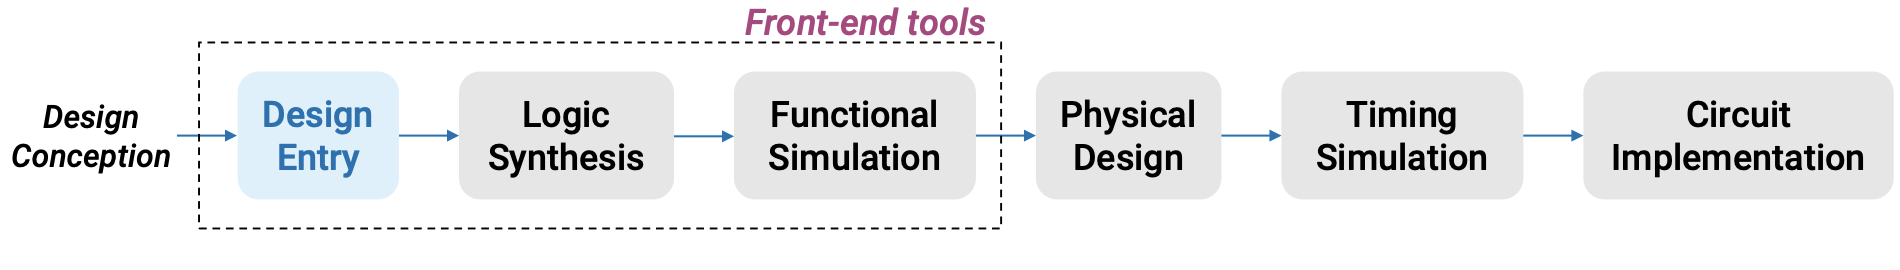
\includegraphics[width=0.67\textwidth]{circuits/10.1.png}
			      	\end{center}
			      	
			      	
			      	
			      	\begin{itemize}
			      		\item[]\textbf{Front End Tools:}
			      		      \begin{itemize}
			      		      	\item \textbf{Design Entry:} The journey begins with the design entry, where the initial concept is articulated. This stage leverages intuition and experience, often utilizing Schematic Capture for graphical representations or Hardware Description Languages (HDLs) like Verilog and VHDL for textual descriptions.
			      		      	\item \textbf{Logic Synthesis:} The design is then transformed into a logic gate structure, where HDL codes are converted into networks of logic gates. This process not only mirrors the intended circuit functionality through logic expressions but also optimizes the design for speed, size, and power efficiency.
			      		      	\item \textbf{Functional Simulation:} This phase verifies the logical correctness of the design by simulating logic functions. Assuming perfect gates, it generates timing waveforms for detailed analysis, ensuring the design operates as expected under ideal conditions.
			      		      \end{itemize}
			      		\item[]\textbf{Back End Tools:}
			      		      \begin{itemize}
			      		      	\item \textbf{Physical Design:} Subsequently, the focus shifts to the physical layout, where the logic expressions are mapped onto a chip using available components. This involves the strategic placement of components and routing connections between them.
			      		      	\item \textbf{Timing Simulation:} This step is crucial to ensure the design meets all timing constraints, accounting for the physical realities of circuit implementation.
			      		      	\item \textbf{Circuit Implementation:} The final step is the circuit's physical realization, where the design is brought to life in hardware form.
			      		      \end{itemize}
			      	\end{itemize}
			    
			      	\section{Verilog HDL}
					\textit{Personal Remark. this course will absolutely NOT suffize to make you a Verilog expert, please take some time to practice in an empty project, just representing in both structural and behavioral ways the circuits we've seen so far. }
			      	\subsection{Structural Modeling with Logic Gates}
			      	In structural modeling, we use predefined modules (\textit{built-in representations of basic logic gates}) to construct complex circuits.\newline
			      	\vspace{5px}
			      	We use this logic gate instantiation statement to create a basic logic gate:
\begin{vhdl}
gate_name [instance_name] (out_port, in_port{, in_port});
\end{vhdl}
			      	[] indicates an optional parameter.\newline
			      	()  indicates a required parameter. \newline
			      	\{\} indicates that additional parameters can be added. \newline
			      	\vspace*{10px}
			      	With \textit{gate\_name} as the type of gate :\newline
			      	\textit{(not limited to these...)}
			      	\begin{center}
			      		\begin{tabular}{|c|c|}
			      			\hline
			      			and  & nor  \\
			      			nand & buf  \\
			      			xor  & not  \\
			      			or   & xnor \\
			      			\hline
			      		\end{tabular}
			      	\end{center}
			      	
			      	\subsubsection{Examples}
			      	
			      	\begin{itemize}
\item[-] \textbf{AND Gate}:
    \begin{vhdl}
    and and1 (out, in1, in2);
    \end{vhdl}
\item[-] \textbf{OR Gate}:
    \begin{vhdl}
    or or1 (out, in1, in2);
    \end{vhdl}
\item[-] \textbf{NOT Gate}:
    \begin{vhdl}
    not not1 (out, in);
    \end{vhdl}
\item[-] \textbf{NAND Gate}:
    \begin{vhdl}
    nand nand1 (out, in1, in2);
    \end{vhdl}
			      	\end{itemize}
			      	\newpage
			      	\subsection{Verilog Syntax}
			      	\textbf{In a Nutshell}
			      	\begin{itemize}
			      		\item[] \textbf{Naming Rules:}
			      		      \begin{itemize}
			      		      	\item[] Begin with a letter.
			      		      	\item[] Include letters, digits, underscore (\_), and dollar sign (\$).
			      		      \end{itemize}
			      		        
			      		\item[] \textbf{Case Sensitivity:}
			      		      \begin{itemize}
			      		      	\item[] Lowercase and uppercase are distinct (e.g., \texttt{a} $\neq$ \texttt{A}).
			      		      \end{itemize}
			      		        
			      		\item[] \textbf{Style Guidelines:}
			      		      \begin{itemize}
			      		      	\item[] Syntax is flexible with white spaces and line breaks.
			      		      	\item[] Prioritize readability with proper indentation.
			      		      \end{itemize}
			      		        
			      		\item[] \textbf{Comments:}
			      		      \begin{itemize}
			      		      	\item[] Initiated by double slashes (//).
			      		      \end{itemize}
			      	\end{itemize}

			      	\subsection{Modules in Verilog}
			      	A circuit or subcircuit described in Verilog is encapsulated within a module. The module declaration includes the module name and its ports, which are the input and output connections to the module.
			      	\begin{vhdl}
module module_name [(port_name{, port_name})];
[input declarations]
[output declarations]
[wire declarations]
[logic gate instantiations]
[module instantiations]
endmodule
			      	\end{vhdl}
			      	\textit{(words in purple are reserved keywords, words after two slashes are comments)} 
			  
			      	\subsection{Ports in Verilog}
			      	Ports are the input and output connections of a module. They are declared within the module declaration
			      	They can be in the following directions :
			      	\textbf{Port Types:}
			      	\begin{itemize}
			      		\item[-] \texttt{input} -- for receiving signals.
			      		\item[-] \texttt{output} -- for sending signals.
			      		\item[-] \texttt{inout} -- for bi-directional signal flow.
			      	\end{itemize}
			      	
			      	\textbf{Port Declaration:}
			      	\begin{itemize}
			      		\item[-] Syntax: 
			      		      \begin{vhdl}
port\_direction data\_type [port\_size] port\_name;
			      		      \end{vhdl}
			      		\item[-] Implicit type: Unspecified types default to wire.
			      		\item[-] Vectors: Specify bit-width for multi-bit signals (e.g., [3:0] for 4 bits).
			      	\end{itemize}
			      	
			      	\textbf{Examples:}
			      	\begin{verbatim}
input diff;            // Single-bit input named diff
inout [15:0] data;     // 16-bit bidirectional port named data
output [3:0] f;        // 4-bit output named f
			      	\end{verbatim}
			      	
			      	\subsection{Example - Full adder in Verilog}
			      	\noindent
			      	\begin{adjustbox}{valign=t,minipage={.5\textwidth}}
			      		\begin{vhdl}
// Structural modeling of a full-adder
module fulladd (a, b, c_in, s, c_out);
// ----- port definitions -----
input a, b, c_in;
output s, c_out;
// ----- intermediate signals -----
wire w1, w2, w3;
// ----- design implementation -----
and And1 (w1, a, b);
and And2 (w2, a, c_in);
and And3 (w3, b, c_in);
or Or1 (c_out, w1, w2, w3);
xor Xor1 (s, a, b, c_in);
endmodule

			      		\end{vhdl}
			      	\end{adjustbox}
			      	\hfill
			      	\begin{adjustbox}{valign=t}
			      		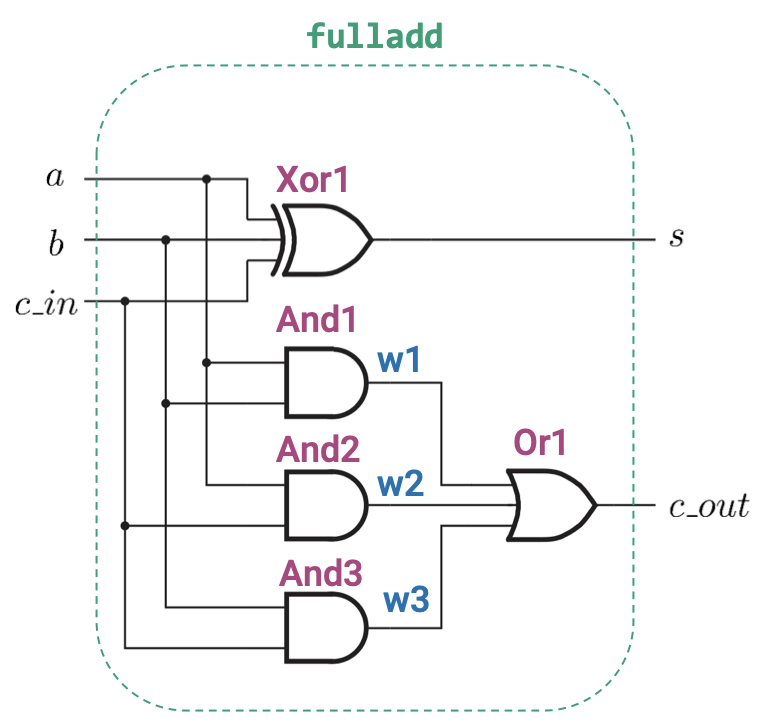
\includegraphics[width=.45\textwidth]{circuits/10.2.4.png}
			      	\end{adjustbox}
			      	Which can be simplified to :\newline \vspace*{5px}
			      	\begin{minipage}{0.4\textwidth}
			      		
			      		\noindent
			      		\begin{vhdl}
module fulladd (a, b, c_in, s, c_out);
input a, b, c_in;
output s, c_out;
and (w1, a, b);
and (w2, a, c_in);
and (w3, b, c_in);
or (c_out, w1, w2, w3);
xor (s, a, b, c_in);
endmodule
			      		\end{vhdl}
			      	\end{minipage}
			      	\subsection{Subcircuits in Verilog}
			      	
			      	\begin{itemize}
			      		\item[] A Verilog module can be included as a subcircuit in another module.
			      		\item[] Modules should be defined in the same source file, or the Verilog compiler must know the locations of the modules.
			      		\item[] Module instantiation syntax:
			      		      \begin{itemize}
			      		      	\item[] \begin{vhdl}
{module\_name instance\_name ( .port\_name (expression));}
			      		      	\end{vhdl}
			      		      	\item[\textbf{Notes:}]
			      		      	      \begin{itemize}
			      		      	      	\item \texttt{module\_name} and \texttt{instance\_name} are any valid identifiers.
			      		      	      	\item \texttt{.port\_name} specifies the subcircuit's port to be connected.
			      		      	      	\item Omitting \texttt{.port\_name} is possible if port order is identical to the subcircuit's definition, but not recommended due to error-proneness.
			      		      	      \end{itemize}
			      		      \end{itemize}
			      	\end{itemize}
			      	
			      	\subsection{Example - Ripple-Carry Adder in Verilog}
			      	A four-bit ripple-carry adder is composed of four full-adder stages with interconnections for the carry bits.
			      	
			      	
			      	\begin{center}
			      		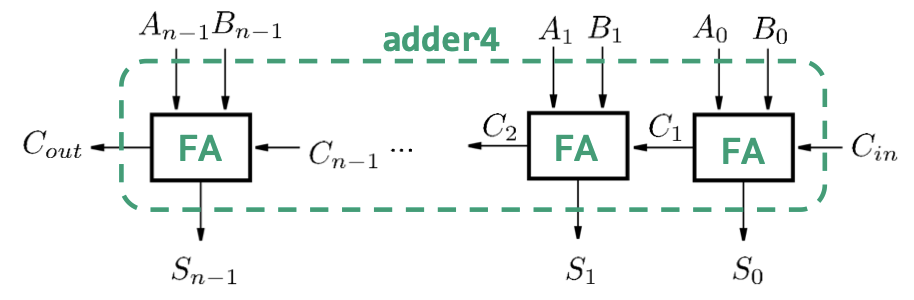
\includegraphics[width=0.70\textwidth]{circuits/10.2.4_2.png}
			      	\end{center}
			      	
			      	Written in VHDL : 
			      	\begin{vhdl}
module adder4 (Cin, A, B, S, Cout);
// Port definitions
input Cin;
input [3:0] A, B; // 4-bit vectors
output [3:0] S;   // 4-bit vector
output Cout;

// Intermediate signals
wire [3:1] C; // 3-bit vector for carry bits

// Design implementation using full-adder stages
fulladd stage0 (.c_in(Cin), .a(A[0]), .b(B[0]), .s(S[0]), .c_out(C[1]));
fulladd stage1 (.c_in(C[1]), .a(A[1]), .b(B[1]), .s(S[1]), .c_out(C[2]));
fulladd stage2 (.c_in(C[2]), .a(A[2]), .b(B[2]), .s(S[2]), .c_out(C[3]));
fulladd stage3 (.c_in(C[3]), .a(A[3]), .b(B[3]), .s(S[3]), .c_out(Cout));
endmodule
			      	\end{vhdl}
			      	
			      	
					
			      	\chapter{Digital Logic and Verilog(PART VI)}

					\section{Bus Architecture}

					  \begin{minipage}{0.48\textwidth}
						  A bus is a communication system that transfers data between components of a digital device. It is designed to connect parts of the motherboard or to link other hardware. In essence:
						  \begin{itemize}
							  \item A bus allows sequential data transmission from multiple sources to various destinations.
							  \item Buses usually carry multiple bits simultaneously, typically more than one bit, to transmit data.
						  \end{itemize}
						  Within Verilog design, multiple-bit wires are termed as \textit{vectors}, and single-bit wires are called \textit{scalars}.
					  \end{minipage}
					  \hfill
					  \begin{minipage}{0.48\textwidth}
						  \centering
						  \includegraphics[width=\textwidth]{circuits/11.1.png} % Replace with actual file path
						  \captionof*{figure}{Illustration of an \(n\)-bit bus}
					  \end{minipage}
										  
					  \subsection{Using Multiplexers (MUXes)}
					  Multiplexers, or MUXes, direct signals from several input lines to a single output line. They select which input to transmit based on control signals.

					  \begin{minipage}{0.48\textwidth}
						A multiplexer can manage multiple \(n\)-bit data lines by using a select signal of \(m\) bits, where \(m\) is the minimum number of bits required to represent the number of inputs, calculated as \(m = \left\lceil \log_2(K) \right\rceil\).

					\end{minipage}
					\hfill
					\begin{minipage}{0.48\textwidth}
						\includegraphics[width=\textwidth]{circuits/11.1.1.png} % Replace with actual file path

					\end{minipage}
					  
					  \subsection{Without Multiplexers} 
					  
					  Buses enable communication between different modules. However, directly connecting two outputs to one input can cause a short-circuit if they attempt to send conflicting signals. Employing multiplexers or tri-state drivers prevents this by ensuring that only one signal is transmitted at a time.
					  
\section{Tri-State Drivers}
\text{
A tri-state driver has a data \textbf{input} $w$, \textbf{output} $f$, and an \textbf{enable} $e$ input.}
\textit{When inactive, a tri-state driver's output enters a high-impedance state (Z), thus three possible states being logical 0, logical 1, or Z.}
\newline
\vskip 10px
\begin{minipage}{0.25\textwidth}
	\hspace*{40px}
\centering
\includegraphics[width=\textwidth]{circuits/11.2.png} % Replace with actual file path

\end{minipage}
\hfill
\noindent
\begin{vline}
	\begin{minipage}{0.48\textwidth}
		\begin{center}
		Thus the following table:
		\vskip 10px
	
		\begin{tabular}{|c|c|c|c|}
			\hline
			e & w & f \\
			\hline
			0 & 0 & Z  \\
			0 & 1 & Z  \\
			1 & 0 & 0  \\
			1 & 1 & 1  \\
			\hline
		\end{tabular}
	\end{center}
	\hspace*{40px}
	\end{minipage}
\end{vline}

\subsection{Types of Tri-State Drivers}


	\begin{minipage}{0.3\textwidth}
	\begin{center}
		\textit{Enable active high} \newline \textit{with inverted f}
	\end{center}
		\centering
	\includegraphics[width=0.6\textwidth]{circuits/11.2.1.png} % Replace with actual file path
	
		\begin{tabular}{|c|c|c|c|}
			\hline
			e & w & f \\
			\hline
			0 & 0 & Z  \\
			0 & 1 & Z  \\
			1 & 0 & 1  \\
			1 & 1 & 0  \\
			\hline
		\end{tabular}
		\hfill
	\end{minipage}
\begin{vline}
\begin{minipage}{0.3\textwidth}
	\vskip 5px
	\begin{center}
		\textit{Enable active low}
	\end{center}
	\centering
\includegraphics[width=0.6\textwidth]{circuits/11.2.1_2.png} % Replace with actual file path

	\begin{tabular}{|c|c|c|c|}
		\hline
		e & w & f \\
		\hline
		0 & 0 & 0  \\
		0 & 1 & 1  \\
		1 & 0 & Z  \\
		1 & 1 & Z  \\
		\hline
	\end{tabular}


\hfill
\end{minipage}
\end{vline}
\noindent
\begin{vline}
	\begin{minipage}{0.3\textwidth}
		\begin{center}
			\textit{Enable active low} \newline \textit{with inverted f}
		\end{center}
	
		\vskip -10px
		\centering
	\includegraphics[width=0.6\textwidth]{circuits/11.2.1_3.png} % Replace with actual file path
	
		\begin{tabular}{|c|c|c|c|}
			\hline
			e & w & f \\
			\hline
			0 & 0 & 1  \\
			0 & 1 & 0  \\
			1 & 0 & Z  \\
			1 & 1 & Z  \\
			\hline
		
		\end{tabular}
		\hfill
	\end{minipage}
\end{vline}

\section{Complete Verilog Built-In Gate List}
Now we can complete the Verilog built-in gate list presented in the last chapter as follows :
\begin{center}
	\begin{tabular}{c|c|c}
		and  & nor & bufif0(f, w, e)  \\
		nand & buf & bufif1(f, w, e)  \\
		xor  & not & notif0(f, w, e) \\
		or   & xnor & notif1(f, w, e) \\
	\end{tabular}

\end{center}

\newpage
\section{Implementing a Bus with Tri-State Drivers}

\noindent % Ensures no indentation at the start of the minipage
\begin{minipage}[htp]{0.4\textwidth}
  In digital systems, a bus with tri-state drivers facilitates selective data transfer between modules without conflict. 
  \vskip 10px
	Each module connects via a driver that outputs high impedance to avoid bus contention, controlled by unique enable signals. (\textit{simplified: one signal at a time})
\end{minipage}\hfill
\begin{minipage}[htp]{0.6\textwidth}
  \centering
  \includegraphics[width=0.8\textwidth]{circuits/11.4.png} % Replace with the actual path to your image
\end{minipage}


\section{Verilog Part 2.}

\subsection{Scalar Signal Values}
Verilog supports one-bit signals (scalars), each signal can have one of the following values:
\begin{center}
	\begin{tabular}{cc}
	\hline
	Value & Meaning \\
	\hline
	0 & Logic 0 \\
	1 & Logic 1 \\
	x & Unknown logic value or don't care \\
	z & tri-state, high-impedance \\
	\hline
\end{tabular}
\end{center}
\subsection{Vector Signal Values}
The value of a vector variable looks like this 
\begin{vhdl}
[size]['radix]constant
\end{vhdl}
$size$ is the number of bits, $radix$ is the base of the number, and $constant$ is the value of the number.
Supported radices include: 
\newline
\begin{center}
	\begin{tabular}{cc}
	\hline
	Radix & Meaning \\
	\hline
	d & decimal \textit{default if no radix is specified} \\
	b & binary \\
	h & hexadecimal \\
	o & octal \\
	\hline
\end{tabular}
\end{center}

\subsection{Parameters}
Parameters are constants that can be used in the module. They are defined as follows:
\begin{vhdl}
parameter name = value;
\end{vhdl}
eg. 
\begin{vhdl}
parameter c = 8;
\end{vhdl}

\subsection{Nets}
Nets are used to connect modules. 
There are two net types:\newline

\vskip 10px
\noindent
\begin{adjustbox}{valign=t,minipage={.45\textwidth}}
	\textit{wires} 
\begin{vhdl}
wire [3:0] a;
\end{vhdl} 
\end{adjustbox}
\hfill
\hskip-10px
\vline
\hfill
\noindent
\begin{adjustbox}{valign=t,minipage={.45\textwidth}}
	\textit{tri-states}
\begin{vhdl}
tri z1 
\end{vhdl}
\end{adjustbox}

\subsection{Behavioral Modeling in Verilog}

Behavioral modeling in Verilog is one of the three modeling paradigms used in Verilog to describe digital circuits at a high level. This approach allows designers to specify how circuits should behave through procedural statements, similar to software programming. 
\textit{Simplified: used when too hard to do in structural modeling.}  


\subsection{Bit-wise Operators}
Bit-wise operators in Verilog are used to perform operations on individual bits of a vector. The following are the bit-wise operators available in Verilog:
\begin{center}
	\begin{tabular}{|c|c|}
		\hline
		Operator & Description \\
		\hline
		\& & Bit-wise AND \\
		| & Bit-wise OR \\
		\^{} & Bit-wise XOR \\
		\~{} & Bit-wise NOT \\
		\hline
	\end{tabular}
\end{center}

\subsection{Example - Structural to Behavioral Modeling}
Here's a circuit we've modeled in structural modeling :
\subsubsection*{Structural}
\vskip 10px
\noindent
\begin{adjustbox}{valign=t,minipage={.45\textwidth}}
\begin{center}
\includegraphics[width=0.9\textwidth]{circuits/11.5.7.png}
\end{center}
\end{adjustbox}
\hfill
\hskip-40px
\vline
\hfill
\noindent
\begin{adjustbox}{valign=t,minipage={.50\textwidth}}
\begin{vhdl}
	module my_circuit_structural (
		input x1, x2, x3, x4,
		output f
		);
		wire w1, w2, w3, w4, w5, w6, w7, w8;
		and (w1, x1, x3);
		not (w2, x2);
		not (w3, x3);
		and (w4, x2, x4);
		or (w5, x1, w3);
		or (w6, w2, x4);
		or (w7, w1, w4);
		and (w8, w5, w6);
		or (f, w7, w8);
		endmodule
\end{vhdl}
\end{adjustbox}
\vspace*{10px}
\subsubsection*{Behavioral}
\begin{vhdl}
module my_circuit_behavioral (
	input x1, x2, x3, x4,
	output f
	);
	wire w7, w8;
	assign w7 = (x1 & x3) | (x2 & x4);
	assign w8 = (x1 | ~x3) & (~x2 | x4);
	assign f = w7 | w8;
endmodule
\end{vhdl}

\subsection{Continuous Assignments in Verilog}
\textbf{Keyword:} \texttt{assign}
\subsubsection*{Definition}
Continuous assignments are used in Verilog for assigning values to wires. The \texttt{assign} statement makes the left-hand side (LHS) of the assignment dynamically reflect any changes in the right-hand side (RHS) immediately.

\subsubsection*{Properties}
\begin{itemize}
    \item[-] Executes continuously: The assignment reacts to any change in the RHS variables and updates the LHS accordingly.
    \item[-] Operates in parallel: The execution order in the code does not affect the simulation behavior.
\end{itemize}

\subsubsection*{Example}
Consider the case where we want to perform a logical OR operation between two signals, \texttt{w7} and \texttt{w8}, and assign the result to signal \texttt{f}:

\begin{vhdl}
assign f = w7 | w8;
\end{vhdl}

In this example, whenever the value of \texttt{w7} or \texttt{w8} changes, \texttt{f} is automatically recalculated to reflect the new value.



\newpage
\subsection{Verilog Always Block}
\textbf{Keyword:} \texttt{always} \newline
\vskip 5px
The \texttt{always} block in Verilog is used for modeling combinational and sequential logic. It reacts to changes in input signals, ensuring that the block's internal logic is evaluated whenever necessary.

\subsubsection*{Structure}
\begin{vhdl}
always @*
	[begin]
	[procedural assignment statements]
	[if-else statements]
	[case statements]
	[while, repeat, and for loops]
	[task and function calls]
[end]
\end{vhdl}

In this block, the \texttt{always} keyword is followed by \texttt{@*}.

\subsection{If-Else Statements}
\textit{Personal Remark. uhm if you've been here until now I think you won't have much trouble understanding this...} \newline
If an expression is true, the code within the begin-end block runs; multiple statements can be grouped in such a block. Optional else if and else clauses, when used, connect to the closest preceding if or else if statement.
\noindent
\subsubsection{Structure}
\begin{vhdl}
if (expression1)
begin
	statement;
end
else if (expression2)
begin
	statement;
end
else
begin
	statement;
end
\end{vhdl}

\newpage
\begin{adjustbox}{valign=t,minipage={1\textwidth}}
\subsection{Example - 2-to-1 MUX}
Using what we've learned so far
\newline 
\begin{adjustbox}{valign=t,minipage={.40\textwidth}}
\begin{center}
\includegraphics[width=0.8\textwidth]{circuits/6.12.2_2.png}
\end{center}
\end{adjustbox}
\hspace*{-40px}
\hfill
\vline
\hfill
\noindent
\begin{adjustbox}{valign=t,minipage={.40\textwidth}}
\begin{vhdl}
module my_2to1mux ( input w1, w2, s, output reg f );
	always @*
		begin
		if (s == 0) 
		begin
			f = w1; 
		end
		else 
		begin
			f = w2; 
		end
	end
endmodule
\end{vhdl}
\end{adjustbox}
\end{adjustbox}
\vspace*{-20px}
\begin{adjustbox}{valign=t,minipage={1\textwidth}}
\subsection{Case Statement} 
\textit{Personal Remark. Switch in java} \newline
\vspace{-10px}
\subsubsection{Syntax}
\begin{vhdl}
case (expression)
    alternative1:
	begin
        statements;
    end
    alternative2: 
	begin
        statements;
    end
    default: 
	begin
        statements;
    end
endcase
\end{vhdl}
\end{adjustbox}
\vfill
\begin{adjustbox}{valign=t,minipage={0.9\textwidth}}
\begin{adjustbox}{valign=t,minipage={.40\textwidth}}
\vfill
\subsubsection{Example - Full Adder}
\vskip 5px
Using the truth table of a Full-Adder, let's use a case statement to implement it:
\begin{center}
\begin{tabular}{|c|c|c||c|c|}
		\hline
		$x$ & $y$ & $C_{in}$ & $s$ & $C_{out}$ \\
		\hline
		0 & 0 & 0 & 0 & 0 \\
		0 & 0 & 1 & 1 & 0 \\
		0 & 1 & 0 & 1 & 0 \\
		0 & 1 & 1 & 0 & 1 \\
		1 & 0 & 0 & 1 & 0 \\
		1 & 0 & 1 & 0 & 1 \\
		1 & 1 & 0 & 0 & 1 \\
		1 & 1 & 1 & 1 & 1 \\
		\hline
\end{tabular}
\end{center}
\vfill
\end{adjustbox}
\hfill
\noindent
\begin{adjustbox}{valign=t,minipage={.50\textwidth}}
\small
\begin{vhdl}
module fulladd (input x, y, Cin, output reg s, Cout);
	always @*
	begin
		case ({x, y, Cin})
		3'b000: {s, Cout} = 'b00;
		3'b001: {s, Cout} = 'b10;
		3'b010: {s, Cout} = 'b10;
		3'b011: {s, Cout} = 'b01;
		3'b100: {s, Cout} = 'b10;
		3'b101: {s, Cout} = 'b01;
		3'b110: {s, Cout} = 'b01;
		3'b111: {s, Cout} = 'b11;
		endcase
	end
endmodule
\end{vhdl}
\end{adjustbox}
\end{adjustbox}


\chapter{Digital Logic and Verilog(PART VII)}

\section{Memory Elements}
\subsection{Introduction - Example Application: Alarm System Control}

Suppose we wish to control an alarm system. The system design involves a \textbf{sensor}, an \textbf{alarm control circuit}, and an \textbf{alarm} indicator. Below is the functional description of the system:

\begin{figure}[h]
	\centering
	\includegraphics[width=0.8\textwidth]{circuits/12.1.1.png}
	\caption{Diagram of the Alarm System Control}
	\end{figure}
\begin{itemize}
  \item[-] The \textbf{sensor} detects an undesirable event and sends a \texttt{SET} signal (logic high or 1) to the \textbf{alarm control circuit}.
  \item[-] The \textbf{alarm control circuit} activates the alarm when it receives the \texttt{SET} signal. The \texttt{ALARM\_ON} signal becomes 1 (logic high), indicating that the alarm is active.
  \item[-] The alarm remains active until a \texttt{RESET} signal (logic high or 1) is sent to the \textbf{alarm control circuit}, turning off the alarm (\texttt{ALARM\_ON} becomes 0).
  \item[-] A memory element in the circuit ensures that the alarm remains active until it is explicitly reset, even if the \texttt{SET} signal goes back to low (0).
\end{itemize}

\vspace*{30px}
\subsection{Combinational vs. Sequential Circuits}
Previously, in \textbf{combinational circuits}, outputs only depended on the current inputs. \newline
\vskip 5px
In \textbf{sequential circuits}, outputs are determined by both the current inputs and the circuit's past behavior, due to the inclusion of memory elements.

\vspace*{10px}
\begin{minipage}{0.45\textwidth}
    Combinational Circuits are memory-less; outputs only depend on the current inputs.
    \begin{center}
        \includegraphics[width=\linewidth]{circuits/12.1.2.png}
    \end{center}
\end{minipage}
\hfill
\vline
\hfill
\begin{minipage}{0.45\textwidth}
	Sequential circuits have memory elements, outputs depend on both current inputs and past behavior.  
	\begin{center}
		\includegraphics[width=\linewidth]{circuits/12.1.2_2.png}
	\end{center}
\end{minipage}

\vspace*{10px}

\begin{justify}
	\textit{Storage elements in a circuit hold logic signal values, defining the circuit's state. When inputs change, the circuit may maintain its current state or transition to a new state. Consequently, the circuit evolves through various states over time based on input changes.}	
\end{justify}

\subsection{Basic Memory Element}
\subsubsection{Bistable Element}
\textit{We're finally storing data !} \newline
We've seen that two Not gates in a series doesn't change the input signal, so, what if we connect the output of the second Not gate to the input of the first Not gate? \newline


\vspace*{20px} 
\noindent
\begin{minipage}{0.40\textwidth}
	\begin{center}
		\includegraphics[width=0.80\textwidth]{circuits/12.1.3.png}
	\end{center}
\end{minipage}
\hfill
\vline
\hfill
\begin{minipage}{0.50\textwidth}
	\begin{center}
		\large
		\begin{tabular}{|c|c|}
			\hline
			
			$Q$ & $\overline{Q}$ \\
			\hline
			0 & 1 \\
			1 & 0 \\
			\hline
		\end{tabular}
	\end{center}
\end{minipage}
\newline
\vspace*{15px}
While this already allows the most basic form of memory, it's not very practical, the given value cannot be changed, and it's not very reliable.

\newpage
\subsubsection{Set-Reset Latch with Reset Priority}
The set-reset latch is a memory element that can store one bit of information. It has two inputs: \texttt{S} (set) and \texttt{R} (reset). The latch retains its state until a new input is received. \newline
\vspace*{10px}
\textbf{Components of the Set-Reset Latch:}
\begin{itemize}
	\item[-] \textit{Set Input (\texttt{S}):} When \texttt{S} is high (1), the latch sets to 1.
	\item[-] \textit{Reset Input (\texttt{R}):} When \texttt{R} is high (1), the latch resets to 0.
	\item[-] \textit{Q Output:} The current state of the latch.
	\item[-] \textit{Q-bar Output:} The inverse of the current state of the latch.
\end{itemize}
\textit{What happens when both \texttt{S} and \texttt{R} are high? \newline
R = 1, S = 1: This is generally considered an unwanted or invalid situation for SR latches because it tries to set and reset the latch at the same time, leading to unpredictable behavior. Some designs define this state specifically to avoid ambiguity.}
\vspace*{10px}
\newline
\noindent
\begin{minipage}{0.40\textwidth}
	\begin{center}
		\includegraphics[width=1.2\textwidth]{circuits/12.1.3_2.png}
	\end{center}
\end{minipage}
\hfill
\hspace*{20px}
\vline
\hfill
\begin{minipage}{0.50\textwidth}
	\begin{center}
		\begin{tabular}{|c|c||c|c||c|c|}
			\hline
			$S$ & $R$ & $\bar{R} \cdot S$ & $Q_a$ & $Q_{\text{next}}$ & $Q_{b,\text{next}}$ \\
			\hline
			0 & 0 & 0 & $Q_a$ & $Q_a$ & $\bar{Q_a}$ \\
			0 & 1 & 0 & 0 & 0 & 1 \\
			1 & 0 & 1 & $Q_a$ & 1 & 0 \\
			1 & 1 & 0 & 0 & 0 & 0 \\
			\hline
			\end{tabular}
	\end{center}
\end{minipage}
\newline
\vspace*{10px}

This is how the next state of the latch is calculated, the current state of the latch is $Q_a$ and $Q_b$ and the next state is $Q_{\text{next}}$ and $Q_{b,\text{next}}$ respectively.
\begin{flalign*}
\vline
& Q_{a,next} = \overline{R + Q_b} = \overline{R + \overline{S + Q_a}} &&\\
& = \overline{R} \cdot (S + Q_a) &&\\
& = \overline{R} \cdot S + \overline{R} \cdot Q_a = Q_{next} &&\\
& Q_b = \overline{S + Q_a} &&
\end{flalign*}
\subsubsection{Set-Reset Latch with Set Priority}

\begin{justify}
	The set-reset latch with set priority is similar to the reset-priority latch, but with the priority reversed. The latch sets to 0 when both \texttt{S} and \texttt{R} are high (1).
\end{justify}
\vspace*{10px}
\begin{minipage}{0.40\textwidth}
	\begin{center}
		\includegraphics[width=1.2\textwidth]{circuits/12.1.3_3.png}
	\end{center}
\end{minipage}
\hfill
\hspace*{20px}
\vline
\hfill
\begin{minipage}{0.50\textwidth}
	\begin{center}
		\begin{tabular}{|c|c|c||c|c|}
			\hline
			$S$ & $R$ & $\bar{R} \cdot Q_a$ & $Q_{a,\text{next}}$ & $Q_{b,\text{next}}$ \\
			\hline
			0 & 0 & $Q_a$ & $Q_a$ & $Q_a$ \\
			\hline
			0 & 1 & 0 & 0 & 1 \\
			\hline
			1 & 0 & 0 & 1 & 0 \\
			\hline
			1 & 1 & 0 & 1 & 1 \\
			\hline
			\end{tabular}
	\end{center}
\end{minipage}
\newline
$Q_{next} = S + \bar{R} \cdot Q_a$
\newpage
\section{Latches with a Control Signal}

\begin{justify}
	Gated latches use a control signal to determine when to change their state. When active, the control signal allows the latch to update its state; when inactive, it prevents changes. This helps avoid unwanted oscillations.
\end{justify}
\subsection{Gated D Latch}

\begin{minipage}{0.45\textwidth}
\begin{justify}
When the control signal C is high, the output Q mirrors changes in input D. Otherwise, Q remains constant, retaining its previous value.
\end{justify}
\end{minipage}
\hfill
\vline
\hfill
\begin{minipage}{0.45\textwidth}
	\begin{center}
		\includegraphics[width=0.6\textwidth]{circuits/12.2.1.png}
	\end{center}
\end{minipage}
\subsection{Flip-Flops}
\textit{Personal Remark. Put simply, the first type requires actual C input to determine when to update, while the other type updates Q in response to an event-driven signal, such as a clock signal (refer to the following section about Clock signals for a clearer explanation).}\newline
\subsubsection{D Flip-Flop}
Flip-flops update outputs at specific times, unlike latches. A D flip-flop captures the input from the D signal only during certain clock signal transitions, ensuring stable and predictable outputs. Once the clock triggers (on a rising or falling edge), the output Q immediately matches the input D and maintains this value, unaffected by any further input changes, until the next clock edge.
\vspace*{10px}

\begin{minipage}{0.4\textwidth}
	\begin{center}
		\includegraphics[width=0.6\textwidth]{circuits/12.2.2.png}
		\text{D Flip-Flop sensitive to the rising edge}
	\end{center}
\end{minipage}
\hfill
\vline
\hfill
\begin{minipage}{0.4\textwidth}
	\begin{center}
		\includegraphics[width=0.6\textwidth]{circuits/12.2.2_2.png}
		\text{D Flip-Flop sensitive to the falling edge}
	\end{center}
\end{minipage}

\section{Clock}
Clocks are essential in digital systems for synchronization purposes. The timing of state changes within the system is orchestrated by these clocks.

\subsection{Clock Signal}
A clock signal is a periodic waveform that oscillates between a high state and a low state. It is characterized primarily by its frequency, which dictates how many cycles occur per second, and its duty cycle, which describes the proportion of time the signal is in the high state within a single cycle.

\subsection{Waveform}
The waveform of a clock signal can be described as follows:
\begin{center}
	\includegraphics[width=0.6\textwidth]{circuits/12.3.2.png}
\end{center}
\justify
\begin{itemize}
    \item \textbf{Period:} The period of a clock signal is the duration of one complete cycle of the waveform and is typically measured in seconds or fractions thereof (like nanoseconds, ns). \newline It is denoted by $T_{CLK}$.
    \item \textbf{Frequency:} The frequency of a clock signal is defined as the number of complete cycles it performs per second. Typical units of measurement are Hertz (Hz). \newline Calculated as $f = \frac{1}{T_{CLK}}$, where $T_{CLK}$ is the period.
    \item \textbf{Duty Cycle:} The duty cycle is the percentage of the period during which the clock signal remains in the high state (often 50\%). Calculated as $D = \frac{T_{high}}{T_{CLK}} \times 100\%$.
\end{itemize}



\begin{justify}
	The transition points of the clock signal, especially the rising edge, often trigger state changes within the digital system, coordinating operations and ensuring the system functions correctly and predictably.
\end{justify}

\section{Verilog Part 3.}
\subsection{Update to Always Block}
Updates can take place one after the other, or concurrently, depending on the assignment used : blocking (=) or nonblocking ($\leq$). \newline
\vspace*{-20px}
\subsubsection{Blocking Assignment}
For example:
Here, B is assigned the value of A, then C is assigned the value of B, and finally, D is assigned the value of C. At the end, A = B = C = D.
This is used to model combinational logic (without memory).
\begin{vhdl}
always @ (...sensitivity list...)
begin
	B = A;
	C = B;
	D = C;
end
\end{vhdl}	
\subsubsection{Nonblocking Assignment}

For example:
Changes occur at the same time, so B is assigned the value of A, C is assigned the \textit{old} value of B, and D is assigned the \textit{old} value of C.
This is used to model sequential logic (with memory).
\begin{vhdl}
always @ (...sensitivity list...)
begin
	B <= A;
	C <= B;
	D <= C;
end
\end{vhdl}

\subsubsection{always(*) Blocks} 
(=) Block Statements should be used. \newline
The \texttt{always @*} block is used to model combinational logic, where the output depends only on the current input values. It is sensitive to any change in the input signals.
\begin{vhdl}
// Example: AND gate
always @ (*)
begin
	C = A & B;
end
\end{vhdl}
\subsubsection{always@(posedge Clock) Blocks}
($\leq$) Nonblocking Statements should be used. \newline
Used to describe sequential logic containing flip-flops \newline
\textit{Note: Remember, $\leq$ like the arrow in the Control Input symbol of a D Flip-Flop representation, it's a reminder that the assignment is non-blocking.}
\begin{itemize}
	\item[-] always@(posedge Clock) – always at the rising clock edge
	\item[-] always@(negedge Clock) – always at the falling clock edge
\end{itemize}
\vspace*{5px}
\section{Behavioral Latch and
Flip-Flop Models}
\subsubsection{Basic D Latch}
The output may be affected whenever inputs D or C change (hence the *)
If input C is 0, we do nothing, there is no else clause.
\begin{vhdl}
module Dlatch (
	input D,
	input C,
	output reg Q
	);
	always @ (*)
	begin
		if (C == 1)
		Q <= D;
	end
endmodule
\end{vhdl}
\vspace*{5px}
\subsubsection{D Latch w/ Enable and Asynchronous Clear}
A D Latch with Enable and Asynchronous Clear is a type of digital storage device used in electronic circuits to store a single bit of data. It has a data input (D), a clock input (C), an enable input (CE), and a clear input (CLR). The output (Q) reflects the input data (D) when both the clock (C) and enable (CE) inputs are active (high). The asynchronous clear (CLR) has the highest priority; when activated (high), it immediately resets the output (Q) to 0, regardless of other input conditions.
Thus the Verilog code for this is:
\begin{vhdl}
module Dlatch (input D, input C, input CE, input CLR,output reg Q);
	always @ (*)
	begin
		if (CLR == 1)
			Q <= 0;
		else if ((C == 1) && (CE == 1))
			Q <= D;
	end
endmodule
\end{vhdl}

\subsubsection{Positive-Edge-Triggered D FF}
D Flip-Flop with positive-edge-triggered clock input. The always block is executed on the positive (rising) CLK edge Q gets set to D
\newline
\begin{vhdl}
module Dff (input D, input CLK, output reg Q);
	always @ (posedge CLK)
		begin
			Q <= D;
		end
endmodule
\end{vhdl}


\subsubsection{D FF (Positive-Edge-Triggered) with Asynchronous Clear}
Works the same as before but the use of posedge here means that the always block is also executed if the CLR signal is high immediately without waiting for the next clock edge.
\begin{vhdl}
module Dff (input D, input CLK, input CLR, output reg Q);
	always @ (posedge CLK or posedge CLR)
		begin
			if (CLR == 1)
				Q <= 0;
			else
				Q <= D;
		end
endmodule
\end{vhdl}
\textit{Note: It would be a mistake to omit posedge and execute the always block on any change in CLR. On a 1-to-0 transition on CLR, the else clause would execute and set Q to D even though no CLK edge had occurred}

\subsubsection{D FF with Asynchronous Clear and $\sim$ Q Output}
The exact same but with an additional output $\sim$ Q which is the complementary of Q.
\vspace*{5px}
\newline
\begin{minipage}{0.5\textwidth}

\begin{vhdl}
module Dff (input D, CLK, CLR, output reg Q, QN);
	always @ (posedge CLK or posedge CLR)
	begin
		if (CLR == 1) begin
			Q <= 0;
			QN <= 1; // complementary output
		end
		else begin
			Q <= D;
			QN <= ~D; // complementary output
		end
	end
endmodule	
\end{vhdl}
\end{minipage}
\hfill
\hspace*{-15px}
\vline
\hfill
\hspace*{-60px}
\begin{minipage}{0.40\textwidth}
	\begin{center}
		\includegraphics[width=0.5\textwidth]{circuits/12.4.3.png}
	\end{center}
\end{minipage}

\subsubsection{D FF with Asynchronous Clear and Synchronous Preset}
A D Flip-Flop with Clock Enable and Synchronous Preset updates its output to the data input (D) at each active clock edge (CE) if enabled, or sets the output to a preset value (S) synchronously if the preset condition is active. \vspace*{5px}
\newline If neither S nor CE is active, the output retains its previous value.
\begin{vhdl}
module Dff (input D, input CLK, input S, input CE, output reg Q);
	always @ (posedge CLK)
		if (S == 1)
			Q <= 1;
		else if (CE == 1)
			Q <= D;
endmodule
\end{vhdl}
\subsubsection{Keywords Summary}
Now what we've seen is just a composition of the following keywords,here's a summary of them:
\begin{footnotesize}
\begin{description}
    \item[Asynchronous Clear:] Allows the immediate resetting of the latch or flip-flop output to a low state (0), regardless of the clock or other control signals' states.
    \item[Enable:] An additional control input that allows the latch to either accept new data when high (enabled) or maintain its current state when low (disabled).
    \item[Positive-Edge Triggered:] Indicates that the flip-flop updates its output only at the rising edge of the clock signal. This specificity in timing helps to synchronize the data flow in digital systems, reducing ambiguity and ensuring stability.
    \item[Synchronous Preset:] Similar to asynchronous clear, but the preset operation occurs in sync with the clock. This feature sets the output to a high state (1) during the clock's active edge.
    \item[Complementary Output:] Provides an additional output that is the logical inverse of the main output. This feature simplifies the design of circuits that require the inverse logic state, reducing the need for external inverting components.
\end{description}
\end{footnotesize}
\section{Practical notes}

For effective sequential systems design, it is crucial to avoid latches due to their susceptibility to glitches, potential for output oscillation, and level sensitivity, which can result in multiple output changes within a single clock period. \newline

Instead, use only D flip-flops and combinational logic. Implement separate \texttt{always} blocks, one set for simple D flip-flops and another for potentially complex combinational logic. \newline

Latches (hold of the last value due to bad timing, and if the last value is the initial one, it must be defined) can inadvertently arise in combinational circuits. To prevent this, ensure all variables in \texttt{always@(*)} blocks are assigned initial default values, ensuring consistent logic states before proceeding to specific assignments. \newline 

In sequential logic, always employ nonblocking assignments using the \texttt{<=} operator in \texttt{always} blocks to ensure simulation consistency across multiple blocks, as this method evaluates all right-hand sides before assigning values to the left-hand sides.\newline



\end{document}